\documentclass[11pt]{article}

\usepackage{graphicx}

\usepackage{amsmath,amsfonts,amssymb}

\usepackage{color}
\definecolor{mygreen}{rgb}{0.1,0.5,0.1}
\newcommand{\mygreen}{\color{mygreen}}
\usepackage[colorlinks=true,linkcolor=black,citecolor=black,filecolor=blue,urlcolor=mygreen]{hyperref}

\newcommand{\todo}[1]{{\bf \color{blue} [#1]}}
\newcommand{\alert}[1]{{\bf \color{red} [#1]}}
\newcommand{\newsection}{\clearpage\newpage}

\setlength{\textwidth}{6.2in}
\setlength{\oddsidemargin}{0.3in}
\setlength{\evensidemargin}{0in}
\setlength{\textheight}{8.7in}
\setlength{\voffset}{-.7in}
\setlength{\headsep}{26pt}


% Macros from FVMHP book -- shortened!

\newcommand{\ignore}[1]{}

%------------------
% matrices and vectors:
\newenvironment{vect}{\left[ \begin{array}{c}}{\end{array}\right]}
\newenvironment{rvect}{\left[ \begin{array}{r}}{\end{array}\right]}
\newenvironment{mat2}{\left[ \begin{array}{cc}}{\end{array}\right]}
\newenvironment{mat}{\left[ \begin{array}{ccccccccccccc}}{\end{array}\right]}
\newenvironment{rmat}{\left[ \begin{array}{rrrrrrrrrrrrr}}{\end{array}\right]}
\newenvironment{lmat}{\left[ \begin{array}{lllllllllllll}}{\end{array}\right]}
\newcommand\bcm{\begin{mat}}
\newcommand\ecm{\end{mat}}
\newcommand\brm{\begin{rmat}}
\newcommand\erm{\end{rmat}}
\newcommand\blm{\begin{lmat}}
\newcommand\elm{\end{lmat}}


%------------------
% piecewise definitions --  one of several choices with left brace:
\newenvironment{pwdef}{\left\{ \begin{array}{ll}}{\end{array}\right.}
\newcommand\bpwdef{\begin{pwdef}}
\newcommand\epwdef{\end{pwdef}}
\newcommand\when{&\m{if}}
\newcommand\otherwise{&\m{otherwise}}





%------------------
% new environments
% these don't always seem to be numbered properly!
%  DELETED

%-------------
% misc. macros


\newcommand\bc{\begin{center}}
\newcommand\ec{\end{center}}
\newcommand\bi{\begin{itemize}}
\newcommand\ei{\end{itemize}}
\newcommand\be{\begin{enumerate}}
\newcommand\ee{\end{enumerate}}


%------------------
%
\newcommand{\Fig}[1]{Figure~\ref{fig:#1}}
\newcommand{\Sec}[1]{Section~\ref{sec:#1}}
\newcommand{\m}[1]{~~~\mbox{#1}~\,}
\newcommand\bsplit{\begin{split}}
\newcommand\esplit{\end{split}}
\newcommand{\eqn}[1]{(\ref{#1})}
\newcommand{\eq}{\begin{equation}}
\newcommand{\en}{\end{equation}}
\newcommand{\eqm}{\begin{eqnarray}}
\newcommand{\enm}{\end{eqnarray}}
\newcommand{\eqmno}{\begin{eqnarray*}}
\newcommand{\enmno}{\end{eqnarray*}}
\newcommand{\eqml}[1]{\eql{#1}\begin{array}{rcl}}
\newcommand{\enml}{\end{array}\en}
\newcommand{\eql}{\begin{equation}\label}
\newcommand{\eqsub}[1]{\begin{subequations}\label{#1}\eqm }
\newcommand{\ensub}{\enm\end{subequations}}
\newcommand\nono{\nonumber}


\newcommand{\half}{{\frac{1}{2}}}
\newcommand{\smhalf}{{\small\frac{1}{2}}}
\newcommand{\goto}{\rightarrow}
\newcommand{\vthin}{\vskip 5pt}
\newcommand\vsp{\vskip .1in}
\newcommand\vvsp{\vskip .3in}
\def\hsp{\hskip 5pt}
\def\hhsp{\hskip 15pt}
\newcommand\noaskip{\noalign{\vskip 4pt}}
\newcommand\lp{\left(}
\newcommand\rp{\right)}
\newcommand\eps{\epsilon}
\newcommand\lam{\lambda}
\newcommand\reals{{{\rm l} \kern -.15em {\rm R} }}
\renewcommand{\Re}{\mbox{Re}}
\newcommand\intoinf{\int_0^\infty~}
\newcommand\complex{{\raisebox{.043ex}{\rule{0.07em}{1.56ex}} \hskip -.35em {\rm C}}}
\newcommand\for{\quad\mbox{for}~}
\newcommand\grad{\nabla}
\newcommand\ie{{\sl i.e.}}
\newcommand\eg{{\sl e.g.}}
%\newcommand\u{\upsilon}
\newcommand\intx{\int_{x_1}^{x_2}\,}
\newcommand\intt{\int_{t_1}^{t_2}\,}
\newcommand\intinf{\int_{-\infty}^{\infty}\,}
\newcommand\ddt{\frac{\partial}{\partial t}}
\newcommand\ddx{\frac{\partial}{\partial x}}
\newcommand\ddy{\frac{\partial}{\partial y}}
\newcommand\ddz{\frac{\partial}{\partial z}}
\newcommand{\ok}[1]{O(k^{#1})}
\newcommand{\oh}[1]{O(h^{#1})}
\newcommand{\E}[1]{\times 10^{#1}}
\newcommand\claw{{\sc clawpack}}
\newcommand\amrclaw{{\sc amrclaw}}
\newcommand\matlab{{\sc matlab}}
\newcommand\fortran{{\sc fortran}}



%\newcommand\dx{\partial_x}
\newcommand\dy{\partial_y}
%\newcommand\dt{\partial_t}
\newcommand\Dx{\Delta x}
\newcommand\Dy{\Delta y}
\newcommand\Dz{\Delta z}
\newcommand\Dt{\Delta t}
\newcommand\dtdx{\frac{\Delta t}{\Delta x}}
\newcommand\amax{a_{\max}}
\newcommand\umax{u_{\max}}
\newcommand\rhomax{\rho_{\max}}
\newcommand\intjcell{\int_{x_{j-1/2}}^{x_{j+1/2}}~}
\newcommand\ujp{U_{j+1}}
\newcommand\ujm{U_{j-1}}
\newcommand\unp{U^{n+1}}
\newcommand\uipn{U_{i+1}^n}
\newcommand\uimn{U_{i-1}^n}
\newcommand\uinp{U_i^{n+1}}
\newcommand\uin{U_i^n}
\newcommand\ujpn{U_{j+1}^n}
\newcommand\ujmn{U_{j-1}^n}
\newcommand\ujnp{U_j^{n+1}}
\newcommand\ujnm{U_j^{n-1}}
\newcommand\ujmnp{U_{j-1}^{n+1}}
\newcommand\ujpnp{U_{j+1}^{n+1}}
\newcommand\ujn{U_j^n}
\newcommand\vjmn{V_{j-1}^n}
\newcommand\vjpn{V_{j+1}^n}
\newcommand\vjnp{V_j^{n+1}}
\newcommand\vjn{V_j^n}
\newcommand\vnp{V^{n+1}}
\newcommand\wjmn{W_{j-1}^n}
\newcommand\wjnp{W_j^{n+1}}
\newcommand\wjn{W_j^n}
\newcommand\ejmn{E_{j-1}^n}
\newcommand\ejpn{E_{j+1}^n}
\newcommand\ejnp{E_j^{n+1}}
\newcommand\ejn{E_j^n}
%\newcommand\cjmh{C_{j-1/2}}
%\newcommand\cjph{C_{j+1/2}}
%\newcommand\djmh{D_{j-1/2}}
%\newcommand\djph{D_{j+1/2}}
\newcommand\cjmh{C_{j-1}}
\newcommand\cjph{C_{j}}
\newcommand\djmh{D_{j-1}}
\newcommand\djph{D_{j}}
\newcommand\thjn{\theta_j^n}
\newcommand\xjm{{x_{j-1}}}
\newcommand\xjp{{x_{j+1}}}
\newcommand\xjmh{{x_{j-1/2}}}
\newcommand\xjph{{x_{j+1/2}}}
\newcommand\tnp{{t_{n+1}}}
\newcommand\tnph{t_{n+1/2}}
\newcommand\aij{A_{ij}}

\newcommand\uij{U_{ij}}
\newcommand\uipj{U_{i+1,j}}
\newcommand\uimj{U_{i-1,j}}
\newcommand\uijp{U_{i,j+1}}
\newcommand\uijm{U_{i,j-1}}
\newcommand\uipjm{U_{i+1,j-1}}
\newcommand\uipjp{U_{i+1,j+1}}
\newcommand\uimjp{U_{i-1,j+1}}
\newcommand\uimjm{U_{i-1,j-1}}

\newcommand\uijn{U_{ij}^n}
\newcommand\uijnp{U_{ij}^{n+1}}
\newcommand\uipjn{U_{i+1,j}^n}
\newcommand\uimjn{U_{i-1,j}^n}
\newcommand\uijpn{U_{i,j+1}^n}
\newcommand\uijmn{U_{i,j-1}^n}
\newcommand\uipjmn{U_{i+1,j-1}^n}
\newcommand\uipjpn{U_{i+1,j+1}^n}
\newcommand\uimjpn{U_{i-1,j+1}^n}
\newcommand\uimjmn{U_{i-1,j-1}^n}
\newcommand\luijn{u_{ij}^n}
\newcommand\luijnp{u_{ij}^{n+1}}
\newcommand\fijn{F_{ij}^n}
\newcommand\gijn{G_{ij}^n}
\newcommand\hrho{\hat\rho}
\newcommand\Jsum{\sum_{j=J}^K}
\newcommand\njsum{\sum_{n=0}^\infty\,\sum_{j=-\infty}^\infty\,}
\newcommand\suminf{\sum_{j=-\infty}^\infty\,}
\newcommand\ujln{U_j^{(l)n}}
\newcommand\tun{\tilde u^n}
\newcommand\hh{{\cal H}_k}
\newcommand\dbar{{\cal D}(\bar x,\bar t)}
\newcommand\dnbar{{\cal D}_k(\bar x,\bar t)}
\newcommand\dobar{{\cal D}_0(\bar x,\bar t)}
\newcommand\askgo{\quad\mbox{as}~~k\goto 0}
\newcommand\sjn{\sigma_j^n}
\newcommand\sig{\sigma}
\newcommand\sjmn{\sigma_{j-1}^n}
\newcommand\tpj{\theta_{pj}}
\newcommand\apj{\alpha_{pj}}
\newcommand\sgn{\mbox{sgn}}
\newcommand\minmod{\mbox{minmod}}
\newcommand\sg{{\cal G}}
\newcommand\sh{{\cal H}}
\newcommand\ujt{U_j(t)}
\newcommand\ujpt{U_{j+1}(t)}
\newcommand\ext{e^{-ta\partial_x}}
\newcommand\eyt{e^{-tb\partial_y}}
\newcommand\exyt{e^{-t(a\partial_x + b\partial_y)}}
\newcommand\eA{e^{-tA\partial_x}}
\newcommand\ehA{e^{-\half tA\partial_x}}
\newcommand\eB{e^{-tB\partial_y}}
\newcommand\eAB{e^{-t(A\partial_x + B\partial_y)}}
\newcommand\ekhA{e^{-\half kA\partial_x}}
\newcommand\ekB{e^{-kB\partial_y}}
\newcommand\ekAB{e^{-k(A\partial_x + B\partial_y)}}
\newcommand\hhx{{\cal H}_{k/2}^x}
\newcommand\hy{{\cal H}_{k}^y}
\newcommand\hx{{\cal H}_{k}^x}
%\newcommand\uss{u^{**}}
\newcommand\wset{{\cal W}}
\newcommand\dist{\operatorname{dist}}
\newcommand\kcpt{{\cal K}}
\newcommand\LT{L_{1,{\scriptscriptstyle T}}}
\newcommand\FG{F_{\scriptscriptstyle G}}
\newcommand\uD{u^{\scriptscriptstyle D}}
\newcommand\llw{L_{\scriptscriptstyle LW}}
\newcommand\supp{\mbox{Supp}}
\newcommand\tvt{\mbox{TV}_{\scriptscriptstyle T}}
\newcommand\hun{\hat u^n}
\newcommand\uhs{\hat u^*}
\newcommand\hau{\hat A(u_l,u_r)}
\newcommand\rh{\rho^{1/2}}
\newcommand\FH{F_{\scriptscriptstyle H}}
\newcommand\FL{F_{\scriptscriptstyle L}}
\newcommand\vpj{V_{pj}}
\newcommand\vpjp{V_{pj_p}}
\newcommand\vpjpm{V_{p,j_p-1}}
\newcommand\bpj{\beta_{pj}}
\newcommand\bpjp{\beta_{pj_p}}
\newcommand\bpjpm{\beta_{p,j_p-1}}
\newcommand\sigpj{\sig_{pj}}
\newcommand\sigpjp{\sig_{pj_p}}
\newcommand\sigpjpm{\sig_{p,j_p-1}}
\newcommand\lpj{\hat \lam_{pj}}
\newcommand\rpj{\hat r_{pj}}
\newcommand\nupj{\nu_{pj}}
\newcommand\w{\tilde u}
\newcommand\cj{[\xjmh,\xjph]}
%\newcommand{\ttl}[1]{\begin{tabbing} xxxxxxxx\=\kill \>{\tt #1} \end{tabbing}}
%\newcommand{\ttl}[1]{\begin{tabbing} xxxx\=\kill \>{\tt #1} \end{tabbing}}
\newcommand{\ttl}[1]{\\ ~\hskip 10pt {\tt #1}\\}
\newcommand\kh{\frac{\Delta t}{\Delta x}}
\newcommand\lip{\lambda_i^p}
\newcommand\lamijp{\lambda_{ij}^p}
\newcommand\betaps{\beta^{ps}}
\newcommand\rij{\rho_{ij}}
\newcommand\rimj{\rho_{i-1,j}}
\newcommand\ripj{\rho_{i+1,j}}
\newcommand\rijp{\rho_{i,j+1}}
\newcommand\rijm{\rho_{i,j-1}}
\newcommand\cij{c_{ij}}
\newcommand\cimj{c_{i-1,j}}
\newcommand\cipj{c_{i+1,j}}
\newcommand\cijp{c_{i,j+1}}
\newcommand\cijm{c_{i,j-1}}
\newcommand\qi{\Q_i}
\newcommand\qin{\Q_i^{n}}
\newcommand\qinp{\Q_i^{n+1}}
\newcommand\qimn{\Q_{i-1}^{n}}
\newcommand\qipn{\Q_{i+1}^{n}}
\newcommand\qimnp{\Q_{i-1}^{n+1}}
\newcommand\qipnp{\Q_{i+1}^{n+1}}
\newcommand\bqi{\bar \Q_i}
\newcommand\qim{\Q_{i-1}}
\newcommand\qip{\Q_{i+1}}
\newcommand\qij{\Q_{ij}}
\newcommand\bqij{\bar \Q_{ij}}
\newcommand\qijn{\Q_{ij}^n}
\newcommand\qijnp{\Q_{ij}^{n+1}}

\newcommand\fin{F_i^n}
\newcommand\fipn{F_{i+1}^n}
\newcommand\fij{F_{ij}}
\newcommand\fimj{F_{i-1,j}}
\newcommand\fipj{F_{i+1,j}}
\newcommand\fijp{F_{i,j+1}}
\newcommand\fijm{F_{i,j-1}}
\newcommand\tfij{\tilde F_{ij}}
\newcommand\tfipj{\tilde F_{i+1,j}}
\newcommand\gij{G_{ij}}
\newcommand\gimj{G_{i-1,j}}
\newcommand\gipj{G_{i+1,j}}
\newcommand\gijp{G_{i,j+1}}
\newcommand\gijm{G_{i,j-1}}
\newcommand\tgij{\tilde G_{ij}}
\newcommand\tgijp{\tilde G_{i,j+1}}
\newcommand\tgimj{\tilde G_{i-1,j}}
\newcommand\tgimjp{\tilde G_{i-1,j+1}}
\newcommand\sip{s_i^p}
\newcommand\aip{\alf_i^p}
\newcommand\rip{r_i^p}
%\newcommand\Dfp{\Delta f^+}
%\newcommand\Dfm{\Delta f^-}
%\newcommand\Dfim{\Delta f_i^-}
%\newcommand\Dfip{\Delta f_i^+}
\newcommand\Dfp{{\cal A}^+\Delta q}
\newcommand\Dfm{{\cal A}^-\Delta q}
\newcommand\Dfim{{\cal A}^-\Delta \Q_i}
\newcommand\Dfip{{\cal A}^+\Delta \Q_i}
\newcommand\apd{{\cal A}^+\Delta }
\newcommand\amd{{\cal A}^-\Delta }
\newcommand\adq{{\cal A}\Delta \Q}
\newcommand\apdq{{\cal A}^+\Delta \Q}
\newcommand\amdq{{\cal A}^-\Delta \Q}
\newcommand\bpdq{{\cal B}^+\Delta \Q}
\newcommand\bmdq{{\cal B}^-\Delta \Q}
\newcommand\amdqi{{\cal A}^-\Delta \Q_i}
\newcommand\amdqip{{\cal A}^-\Delta \Q_{i+1}}
\newcommand\apdqi{{\cal A}^+\Delta \Q_i}
\newcommand\Dfpp{\Delta f^{++}}
\newcommand\Dfpm{\Delta f^{+-}}
\newcommand\Dq{\Delta \Q}
\newcommand\Dqi{\Delta \Q_i}
\newcommand\Dqij{\Delta \Q_{ij}}
\newcommand\Df{\Delta f}
\newcommand\DtDy{\frac{\Delta t}{\Delta y}}
\newcommand\DtDx{\frac{\Delta t}{\Delta x}}
\newcommand\W{{\cal W}}
\newcommand\WZ{{\cal Z}}
\newcommand\tW{\widetilde {\cal W}}
\newcommand\Wp{{\cal W}^p}
\newcommand\Wip{{\cal W}_i^p}
\newcommand\Wimp{{\cal W}_{i-1}^p}
\newcommand\Wijp{{\cal W}_{ij}^p}
\newcommand\Wipjp{{\cal W}_{i+1,j}^p}
\newcommand\Wimjp{{\cal W}_{i-1,j}^p}
\newcommand\tWijp{\widetilde {\cal W}_{ij}^p}
\newcommand\tWip{\widetilde {\cal W}_i^p}
\newcommand\tfi{\tilde F_{i}}
\newcommand\tfip{\tilde F_{i+1}}
\newcommand\fip{F_{i+1}}
\newcommand\summ{\sum_{\lam_i^p<0}}
\newcommand\sump{\sum_{\lam_i^p>0}}
\newcommand\msum{\sum_{i=1}^m}
\newcommand\psum{\sum_{p=1}^m}
\newcommand\DGi{\Delta_i^{\mbox{\small up}}}
\newcommand\DGij{\Delta_{ij}^{\mbox{up}}}
\newcommand\Aij{A_{ij}}
\newcommand\Dfijp{{\cal A}^+\Delta \Q_{ij}}
\newcommand\Dfijm{{\cal A}^-\Delta \Q_{ij}}
\newcommand\Dgijp{{\cal B}^+\Delta_y \Q_{ij}}
\newcommand\Dgijm{{\cal B}^-\Delta_y \Q_{ij}}
\newcommand\asdq{{\cal A}^*\Delta \Q}
\newcommand\apdqij{{\cal A}^+\Delta \Q_{ij}}
\newcommand\amdqij{{\cal A}^-\Delta \Q_{ij}}
\newcommand\apmdq{{\cal A}^{\pm}\Delta \Q}
\newcommand\apmdqij{{\cal A}^{\pm}\Delta \Q_{ij}}
\newcommand\amdqipj{{\cal A}^-\Delta \Q_{i+1,j}}
\newcommand\asdqij{{\cal A}^*\Delta \Q_{ij}}
\newcommand\bpdqij{{\cal B}^+\Delta \Q_{ij}}
\newcommand\bmdqij{{\cal B}^-\Delta \Q_{ij}}
\newcommand\bpmdq{{\cal B}^{\pm}\Delta \Q}
\newcommand\bpmdqij{{\cal B}^{\pm}\Delta \Q_{ij}}
\newcommand\bmdqijp{{\cal B}^-\Delta \Q_{i,j+1}}
\newcommand\bpmapdq{{\cal B}^{\pm}{\cal A}^+ \Delta \Q}
\newcommand\bpmamdq{{\cal B}^{\pm}{\cal A}^- \Delta \Q}
\newcommand\apmbpdq{{\cal A}^{\pm}{\cal B}^+ \Delta \Q}
\newcommand\apmbmdq{{\cal A}^{\pm}{\cal B}^- \Delta \Q}
\newcommand\sijp{\lam_{ij}^p}
\newcommand\bmamdq{{\cal B}^-{\cal A}^-\Delta \Q}
\newcommand\bmapdq{{\cal B}^-{\cal A}^+\Delta \Q}
\newcommand\bpamdq{{\cal B}^+{\cal A}^-\Delta \Q}
\newcommand\bpapdq{{\cal B}^+{\cal A}^+\Delta \Q}
\newcommand\bpasdq{{\cal B}^+{\cal A}^*\Delta \Q}
\newcommand\bmasdq{{\cal B}^-{\cal A}^*\Delta \Q}
\newcommand\bpmasdq{{\cal B}^{\pm}{\cal A}^*\Delta \Q}
\newcommand\bpmapmdq{{\cal B}^{\pm}{\cal A}^{\pm}\Delta \Q}
\newcommand\ambsdq{{\cal A}^-{\cal B}^*\Delta \Q}
\newcommand\apbsdq{{\cal A}^+{\cal B}^*\Delta \Q}
\newcommand\bsdq{{\cal B}^*\Delta q}


\newcommand\uimhj{u_{i-1/2,j}}
\newcommand\uiphj{u_{i+1/2,j}}
\newcommand\vimhj{v_{i-1/2,j}}
\newcommand\vijmh{v_{i,j-1/2}}
\newcommand\vijph{v_{i,j+1/2}}
%\newcommand\ql{q^{\scriptstyle L}}
%\newcommand\qr{q^{\scriptstyle R}}
\newcommand\cim{c_{i-1}}
\newcommand\T{{\cal T}}
\newcommand\bu{\bar u}
\newcommand\bv{\bar v}
\newcommand\cfl{CFL}
\newcommand\epixi{e^{i\xi\Dx}}
\newcommand\emixi{e^{-i\xi\Dx}}
\newcommand\epieta{e^{i\eta\Dy}}
\newcommand\emieta{e^{-i\eta\Dy}}
\newcommand\qeps{\q^{\eps}}
\newcommand\tqxi{\tq(\xi)}
\newcommand\dOmega{\partial\Omega}

\newcommand\fup{F^{\mbox{up}}}
\newcommand\bulk{K}

% group equations as (1.1a), (1.1b), etc.
%
\newcounter{equationgroup}
%
\newenvironment{eqngroup}{%
\refstepcounter{equation}%
\setcounter{equationgroup}{\value{equation}}%
\edef\theequationgroup{\theequation}%
\setcounter{equation}0%
\newcommand\theequation{\theequationgroup\alph{equation}}}{%
\setcounter{equation}{\value{equationgroup}}%
\edef\theequation{\theequationgroup}}%
%\global\@ignoretrue}


\newcommand\smax{s_{\text{max}}}
\newcommand\bq{\q_s}
\newcommand\bt{\bar t}
\newcommand\wI{\w^I}
\newcommand\wII{\w^{II}}
\newcommand\tq{\tilde \q}
\newcommand\qjn{\Q_j^n}
\newcommand\qjpn{\Q_{j+1}^n}
\newcommand\akh{\frac{ak}{h}}
\newcommand\uim{U_{i-1}}
\newcommand\uip{U_{i+1}}
\newcommand\uimnp{U_{i-1}^{n+1}}
\newcommand\uipnp{U_{i+1}^{n+1}}
\newcommand\theti{\theta_i}
\newcommand\thetim{\theta_{i-1}}
\newcommand\thetip{\theta_{i+1}}
\newcommand\thetnu{\theta^{[\nu]}}
\newcommand\thetnup{\theta^{[\nu+1]}}
\newcommand\thetzero{\theta^{[0]}}
\newcommand\thethat{\hat\theta}
\newcommand\delnu{\delta^{[\nu]}}
\newcommand\Jnu{J^{[\nu]}}
\newcommand\Jhath{\hat J^h}
\newcommand\q{Q}
%\newcommand\u{u}
\newcommand\Q{Q}
\newcommand\intu{\int_{x_1}^{x_2} \q(x,t)\,dx}
\newcommand\domega{\partial\Omega}
\newcommand\ustar{U^*}
\newcommand\qn{\Q^n}
\newcommand\qnp{\Q^{n+1}}
\newcommand\qnm{\Q^{n-1}}
\newcommand\qnj{\Q^{n+j}}
\newcommand\qnr{\Q^{n+r}}
\newcommand\qimjn{\Q_{i-1,j}^n}
\newcommand\qipjn{\Q_{i+1,j}^n}
\newcommand\qipjpn{\Q_{i+1,j+1}^n}
\newcommand\qipjmn{\Q_{i+1,j-1}^n}
\newcommand\qimjpn{\Q_{i-1,j+1}^n}
\newcommand\qijpn{\Q_{i,j+1}^n}
\newcommand\qijmn{\Q_{i,j-1}^n}
\newcommand\qimj{\Q_{i-1,j}}
\newcommand\qipj{\Q_{i+1,j}}
\newcommand\qijp{\Q_{i,j+1}}
\newcommand\qijm{\Q_{i,j-1}}
\newcommand\qimjm{\Q_{i-1,j-1}}
\newcommand\qipjm{\Q_{i+1,j-1}}
\newcommand\qimjp{\Q_{i-1,j+1}}
\newcommand\qipjp{\Q_{i+1,j+1}}
\newcommand\cond{\text{cond}}
\newcommand\Rinv{R^{-1}}
\newcommand\qnup{\q^{[\nu+1]}}
\newcommand\qnu{\q^{[\nu]}}
\newcommand\qinup{\q_i^{[\nu+1]}}
\newcommand\qinu{\q_i^{[\nu]}}
\newcommand\qimnu{\q_{i-1}^{[\nu]}}
\newcommand\qimnup{\q_{i-1}^{[\nu+1]}}
\newcommand\qipnu{\q_{i+1}^{[\nu]}}
\newcommand\enu{e^{[\nu]}}
\newcommand\enup{e^{[\nu+1]}}
\newcommand\Minv{M^{-1}}
\newcommand\qs{q^*}
\newcommand\ezero{e^{[0]}}
\newcommand\qzero{q^{[0]}}

\newcommand{\hm}[1]{\frac{1}{h^{#1}}}
\newcommand{\Tab}[1]{Table~\ref{tab:#1}}


\newcommand\inttn{\int_{t_n}^{\tnp}}
\newcommand\cell{{\cal C}}
\newcommand\intCi{\int_{\celli}}
\newcommand\ql{q_l}
\newcommand\qr{q_r}
%\newcommand\bu{\bar u}
\newcommand\tqn{\tilde q^n}
\newcommand\lamp{\lam^p}
\renewcommand{\w}{w}
\renewcommand{\wp}{\w^p}
\renewcommand{\l}{\ell}
\newcommand{\qm}{\q_m}
\newcommand{\bx}{\bar x}
%
% from fv.tex
%\newcommand{\minmod}{\text{minmod}}
\newcommand{\talfip}{\tilde \alfip}
\newcommand{\thetaip}{\theta_i^p}
\newcommand{\tF}{\tilde F}
\newcommand{\tG}{\tilde G}
\newcommand{\maxmod}{\text{maxmod}}
\newcommand{\celli}{{\cal C}_i}
\newcommand{\cellim}{{\cal C}_{i-1}}
\newcommand{\bxi}{\bar x_i}
\newcommand{\sigin}{\sigma_i^n}
\newcommand{\sigimn}{\sigma_{i-1}^n}
\newcommand{\sigipn}{\sigma_{i+1}^n}
\newcommand{\bukh}{\frac{\bu k}{h}}
\renewcommand{\q}{q}
\renewcommand{\tq}{\tilde \q}
\newcommand{\tqnp}{\tq^n(x,t_{n+1})}
\renewcommand{\tqn}{\tq^n(x,t_{n})}
\newcommand{\thetain}{\theta_i^n}
\newcommand{\thetaipn}{\theta_{i+1}^n}
\newcommand{\alfip}{\alf_i^p}
\newcommand{\cin}{C_i^n}
\newcommand{\cimn}{C_{i-1}^n}
\newcommand{\cipn}{C_{i+1}^n}
\newcommand{\din}{D_i^n}
\newcommand{\dipn}{D_{i+1}^n}
\newcommand{\delin}{\delta_i^n}
\newcommand{\delipn}{\delta_{i+1}^n}
\newcommand{\Dqin}{\Delta \Q_i^n}
\newcommand{\Dqipn}{\Delta \Q_{i+1}^n}
\newcommand{\D}{\Delta }
\renewcommand{\Dq}{\Delta\Q}
\newcommand{\khbu}{\frac{k\bu}{h}}
\newcommand\vu{\vec u}
\newcommand\vx{\vec x}
\newcommand\dvx{d\vec x}
\newcommand\vE{\vec E}
\newcommand\vsF{\vec {\cal F}}
\newcommand\sF{{\cal F}}
\newcommand\vj{\vec j}
\newcommand\vV{\vec V}
\newcommand\vW{\vec W}
\newcommand\vP{\vec P}
\newcommand\vF{\vec F}
\newcommand\vn{\vec n}
\newcommand\vnimj{\vec n_{i-1/2,j}}
\newcommand{\nnimj}[1]{n_{i-1/2,j}^{#1}}
\newcommand{\nnijm}[1]{n_{i,j-1/2}^{#1}}
\newcommand{\eeimj}[1]{e_{i-1/2,j}^{#1}}
\newcommand{\eeijm}[1]{e_{i,j-1/2}^{#1}}
\newcommand{\veimj}{e_{i-1/2,j}}
\newcommand{\veijm}{e_{i,j-1/2}}
\newcommand\K{K}

\newcommand\xii{\xi_{i-1/2}}
\newcommand\xiip{\xi_{i+1/2}}
\newcommand\fipjn{F_{i+1,j}^n}
\newcommand\fijpn{F_{i,j+1}^n}
\newcommand\gijpn{G_{i,j+1}^n}
\newcommand\hipj{h_{i+1/2,j}}
\newcommand\himj{h_{i-1/2,j}}
\newcommand\hijm{h_{i,j-1/2}}
\newcommand\hijp{h_{i,j+1/2}}
\newcommand\sFipj{{\cal F}_{i+1/2,j}}
\newcommand\sFimj{{\cal F}_{i-1/2,j}}
\newcommand\sFijp{{\cal F}_{i,j+1/2}}
\newcommand\sFijm{{\cal F}_{i,j-1/2}}
\newcommand\bFimj{{\bar F}_{i-1/2,j}}
\newcommand\bFipj{{\bar F}_{i+1/2,j}}
\newcommand\bGijm{{\bar G}_{i,j-1/2}}
\newcommand\bGijp{{\bar G}_{i,j+1/2}}
\newcommand\vsFimj{\vec {\cal F}_{i-1/2,j}}
\newcommand\vsFijm{\vec {\cal F}_{i,j-1/2}}
\newcommand\kapij{\kappa_{ij}}
\newcommand\Dxi{\Delta\xi}
\newcommand\Deta{\Delta\eta}

\newcommand\vijm{v_{i,j-1/2}}
\newcommand\vijp{v_{i,j+1/2}}
\newcommand\vimj{v_{i-1/2,j}}
\newcommand\buimj{\bar u_{i-1/2,j}}
\newcommand\bvijm{\bar v_{i,j-1/2}}
\newcommand\vuimj{\vec u_{i-1/2,j}}
\renewcommand{\uimj}{u_{i-1/2,j}}
\renewcommand{\uijm}{u_{i,j-1/2}}
\renewcommand{\uipj}{u_{i+1/2,j}}
\renewcommand{\vimj}{v_{i-1/2,j}}
\renewcommand{\vijm}{v_{i,j-1/2}}
\renewcommand{\vijp}{v_{i,j+1/2}}

\newcommand{\bfe}[1]{{\bf e}_{#1}}
\newcommand{\bfnor}[1]{{\bf n}_{#1}}
\newcommand\bfbu{{\bf \bar u}}
\newcommand\bfbw{{\bf \bar w}}
\newcommand\bfu{{\bf u}}
\newcommand\bfbn{{\bf \bar n}}
\newcommand\bfbd{{\bf \bar \delta}}
\newcommand\bfd{{\bf \delta}}
\newcommand\bfdxi{{\bf d\xi}}
\newcommand\bfdeta{{\bf d\eta}}
\newcommand\xiim{\xi_{i-1/2,j}}
\newcommand\etajm{\eta_{i,j-1/2}}
\newcommand\etajp{\eta_{i,j+1/2}}

\newcommand\eimj{e_{i-1/2,j}}
\newcommand\Xxi{X_{\xi}}
\newcommand\Xeta{X_{\eta}}
\newcommand\Yxi{Y_{\xi}}
\newcommand\Yeta{Y_{\eta}}
\newcommand\sinth{\sin\theta}
\newcommand\costh{\cos\theta}

%
\newcommand{\spd}{s}
\newcommand{\spdimh}{s\imh}

\newcommand{\bigo}{{\mathcal O}}
%\newcommand{\bigoh}{{\mathcal O}}

%\newcommand{\exweb}{\fbox{WWW}}
\newcommand{\exweb}{ }
%\newcommand{\book}{notes}
\newcommand{\clawlink}[1]{{\tt [claw/book/chap\thechapter/#1]}}

% capa

\renewcommand{\bq}{\bar q}
\newcommand\simhp{s_{i-1/2}^p}
\newcommand{\bqin}{\bar\Q_{i}^n}
\newcommand{\bqimn}{\bar\Q_{i-1}^n}
\newcommand{\bqipn}{\bar\Q_{i+1}^n}
\newcommand{\bqinp}{\bar\Q_{i}^{n+1}}
\newcommand{\qimh}{\Q_{i-1/2}}
\newcommand{\qiph}{\Q_{i+1/2}}
\newcommand{\qimhn}{\Q_{i-1/2}^n}
\newcommand{\qiphn}{\Q_{i+1/2}^n}
\renewcommand{\qimnp}{\Q_{i-1}^{n+1}}
\newcommand{\tFiphn}{\tilde F_{i+1/2}^n}
\newcommand{\tFimhn}{\tilde F_{i-1/2}^n}
\newcommand{\tFimhjn}{\tilde F_{i-1/2,j}^n}
\newcommand{\tFiphjn}{\tilde F_{i+1/2,j}^n}
\newcommand{\tGijphn}{\tilde G_{i,j+1/2}^n}
\newcommand{\tGijmhn}{\tilde G_{i,j-1/2}^n}
\newcommand{\tFimh}{\tilde F_{i-1/2}}
\newcommand{\tFiph}{\tilde F_{i+1/2}}

\newcommand{\tFimhj}{\tilde F_{i-1/2,j}}
\newcommand{\tFiphj}{\tilde F_{i+1/2,j}}
\newcommand{\tGijmh}{\tilde G_{i,j-1/2}}
\newcommand{\tGijph}{\tilde G_{i,j+1/2}}

\newcommand{\Fimh}{F_{i-1/2}}
\newcommand{\Fiph}{F_{i+1/2}}
\newcommand{\Fimhn}{F_{i-1/2}^n}
\newcommand{\Fiphn}{F_{i+1/2}^n}
\newcommand{\Fiphjn}{F_{i+1/2,j}^n}
\newcommand{\Fimhjn}{F_{i-1/2,j}^n}
\newcommand{\Gijmhn}{G_{i,j-1/2}^n}
\newcommand{\Gijphn}{G_{i,j+1/2}^n}
\newcommand{\lamimhp}{\lambda_{i-1/2}^p}
\newcommand{\tWimh}{\widetilde \W_{i-1/2}}
\newcommand{\tWimhp}{\widetilde \W_{i-1/2}^p}
\newcommand{\tWiphp}{\widetilde \W_{i+1/2}^p}
\newcommand{\Wimhp}{\W_{i-1/2}^p}
\newcommand{\Wiphp}{\W_{i+1/2}^p}
\newcommand{\Wimh}{\W_{i-1/2}}
\newcommand{\Wiph}{\W_{i+1/2}}
\newcommand{\alfpimh}{\alf^p_{i-1/2}}
\newcommand{\alfimh}{\alf_{i-1/2}}
\newcommand{\alfiph}{\alf_{i+1/2}}
\newcommand{\kapi}{\kappa_i}
\newcommand{\kapimh}{\kappa_{i-1/2}}
\newcommand{\kkh}{\frac{\Dt}{\kapi \Dx}}
\newcommand{\DQim}{\Delta\Q_{i-1/2}}

%clawpdes:
\newcommand\brho{\bar\rho}
\newcommand{\tu}{\tilde u}
\newcommand{\tp}{\tilde p}
\newcommand{\trho}{\tilde \rho}
\newcommand{\trhou}{\widetilde{\rho u}}


\newcommand{\amdqimh}{{\cal A}^-\Delta \Q_{i-1/2}}
\newcommand{\apdqimh}{{\cal A}^+\Delta \Q_{i-1/2}}
\newcommand{\amdqiph}{{\cal A}^-\Delta \Q_{i+1/2}}
\newcommand{\apdqiph}{{\cal A}^+\Delta \Q_{i+1/2}}
\newcommand{\apmdqimh}{{\cal A}^{\pm}\Delta \Q_{i-1/2}}
\newcommand{\lamimh}{\lam_{i-1/2}}

%highres:
\renewcommand{\bukh}{\frac{\bu\Dt}{\Dx}}
\renewcommand{\delin}{\delta_{i-1/2}^n}
\renewcommand{\thetain}{\theta_{i-1/2}^n}
\renewcommand{\thetaip}{\theta_{i-1/2}^p}
\renewcommand{\thetaipn}{\theta_{i+1/2}^n}
\renewcommand{\alfip}{\alf_{i-1/2}^p}
\renewcommand{\talfip}{\tilde\alf_{i-1/2}^p}
\renewcommand{\lip}{\lam_{i-1/2}^p}
\renewcommand{\Dqin}{\Delta\Q_{i-1/2}^n}

%vcacou:
\newcommand{\nph}{^{n+1/2}}
%\newcommand{\tnph}{t_{n+1/2}}
\newcommand{\imh}{_{i-1/2}}
\newcommand{\jmh}{_{j-1/2}}
\newcommand{\imhn}{_{i-1/2}^n}
\newcommand{\iph}{_{i+1/2}}
\newcommand{\iphn}{_{i+1/2}^n}
\newcommand{\Zi}{Z_i}
\newcommand{\Zim}{Z_{i-1}}

%curvi:
\newcommand\xieta{(\xi,\eta)}
\newcommand\xideta{$\xi$-$\eta$ }
\newcommand\uub{\bar u}
\newcommand\ulb{\underline u}
\newcommand\vw{\vec w}
\newcommand\wub{\overline w}
\newcommand\wlb{\underline w}
\newcommand\bolde{{\bf e}}
\newcommand\bhate{{\bf\hat e}}
\newcommand\vz{\vec z}
\newcommand\zub{\bar z}
\newcommand\zlb{\underline z}
\newcommand\Jinv{\ensuremath{J^{-1}}}
\newcommand\JinvT{\ensuremath{J^{-T}}}
\newcommand\Ginv{\ensuremath{G^{-1}}}
\newcommand\Mllb{\underline{\underline M}}
\newcommand\Muub{\overline{\overline M}}
\newcommand\Gllb{\underline{\underline G}}
\newcommand\Guub{\overline{\overline G}}
\renewcommand{\aij}{a_{ij}}
\newcommand\Uimj{U^1_{i-1/2,j}}
\newcommand\Uipj{U^1_{i+1/2,j}}
\newcommand\Uijm{U^2_{i,j-1/2}}
\newcommand\Uijp{U^2_{i,j+1/2}}
\newcommand\Vijm{U^2_{i,j-1/2}}
\newcommand\Vijp{U^2_{i,j+1/2}}
\newcommand\bfhimj{{\vec h}_{i-1/2,j}}
\newcommand\bfhipj{{\vec h}_{i+1/2,j}}
\newcommand\bfhijm{{\vec h}_{i,j-1/2}}
\newcommand\bfhijp{{\vec h}_{i,j+1/2}}
\newcommand\ximjm{x_{i-1/2,j-1/2}}
\newcommand\yimjm{y_{i-1/2,j-1/2}}
\newcommand\ximjp{x_{i-1/2,j+1/2}}
\newcommand\yimjp{y_{i-1/2,j+1/2}}
\newcommand\xipjm{x_{i+1/2,j-1/2}}
\newcommand\yipjm{y_{i+1/2,j-1/2}}
\newcommand\ximj{x_{i-1/2,j}}
\newcommand\yimj{y_{i-1/2,j}}
\newcommand\xijm{x_{i,j-1/2}}
\newcommand\yijm{y_{i,j-1/2}}
\newcommand\undergrad{\underline\grad}
%\newcommand\R{{\cal R}}
\newcommand\Wimj{\W_{i-1/2,j}}
\newcommand\lamimj{\lam_{i-1/2,j}}
\newcommand\amdqimj{\amdq_{i-1/2,j}}
\newcommand\apdqimj{\apdq_{i-1/2,j}}
\newcommand\apmdqimj{\apmdq_{i-1/2,j}}


\newcommand\bfn{n}
\newcommand\bfnimj{{\vec n}_{i-1/2,j}}
\newcommand\bfnijm{{\vec n}_{i,j-1/2}}
\newcommand\bfuimj{{\bf u}_{i-1/2,j}}
\newcommand\bfF{{\bf F}}
\newcommand\bfsF{\vec f}
\newcommand\bfsFimj{{{\breve F}_{i-1/2,j}}}
\newcommand\bfsFijm{{{\breve F}_{i,j-1/2}}}
\newcommand\bfimj{{\bf e}_{i-1/2,j}}
\newcommand\bfijm{{\bf e}_{i,j-1/2}}
\newcommand{\bfeimj}{{\bf e}_{i-1/2,j}}
\newcommand{\bfeijm}{{\bf e}_{i,j-1/2}}

% quadril

\newcommand\qsimj{\Q^*_{i-1/2,j}}
\newcommand\qsijm{\Q^*_{i,j-1/2}}
\newcommand\cellij{{\cal C}_{ij}}
\newcommand\cellimj{{\cal C}_{i-1,j}}
\newcommand\cellijm{{\cal C}_{i,j-1}}
\newcommand\gamimj{\gamma_{i-1/2,j}^1}
\newcommand\gamijm{\gamma_{i,j-1/2}^2}
%\newcommand\Uimj{U_{i-1/2,j}}
%\newcommand\Vijm{V_{i,j-1/2}}
\newcommand\cellvol{|{\cal C}|}
\newcommand\cellvolij{|{\cal C}_{ij}|}

% unsplit

\newcommand\intxi{\int_{\ximh}^{\xiph}}
\newcommand\intyj{\int_{\yjmh}^{\yjph}}
\newcommand\ximh{x_{i-1/2}}
\newcommand\xiph{x_{i+1/2}}
\newcommand\yjmh{y_{j-1/2}}
\newcommand\yjph{y_{j+1/2}}
\newcommand\qimjmn{\Q_{i-1,j-1}^n}
\newcommand\intij{\int_{\ximh}^{\xiph}\int_{\yjmh}^{\yjph}}
\newcommand\xim{x_{i-1}}
\newcommand\xip{x_{i+1}}

% sssource

\newcommand\rhovn{\rho_{\scriptscriptstyle vN}}
\newcommand\rhocj{\rho_{\scriptscriptstyle CJ}}
\newcommand\scj{s_{\scriptscriptstyle CJ}}
\newcommand\rhol{\rho_l}
\newcommand\rhor{\rho_r}
\newcommand\Tign{T_{\rm ign}}
\newcommand\rhomerge{\rho_{\rm mrg}}

% bc1
\newcommand\Nn{_N^n}
\newcommand\Npn{_{N+1}^n}
\newcommand\Nmn{_{N-1}^n}
\newcommand\Nphn{_{N+1/2}^n}
\newcommand\Nmhn{_{N-1/2}^n}


% IC's
\newcommand{\ico}[1]{#1 \kern -1ex \raisebox{1.1ex}{$\circ$}}
\newcommand{\icos}[2]{#1 \kern -1.1ex \raisebox{1.1ex}[.5em]{$\circ$}^{#2}}
\newcommand{\icosw}[1]{\bar{w}^{#1}}
%\newcommand{\icosw}[1]{w \kern -1.1ex \raisebox{1.1ex}[.5em]{$\circ$}^{#1}}

% highresacc

\newcommand{\Lode}{{\cal L}}

% vcacou

\newcommand\coeftr{C_{T}}
\newcommand\coefre{C_{R}}
\newcommand\rimhp{r_{i-1/2}^p}
\newcommand\alfimhp{\alf_{i-1/2}^p}

% fvscalar

%\newcommand\qimhs{\Q_{i-1/2}^*}
\newcommand\qimhs{\Qrp\imh}

\newcommand\Dtj{\Dt^{(j)}}
\newcommand\Dxj{\Dx^{(j)}}
\newcommand\Qj{\Q^{(j)}}
\newcommand\Phiin{\Phi_i^n}
\newcommand\intxcell{\int_{x_{i-1/2}}^{x_{i+1/2}}}
\newcommand\QDt{\Q^{(\Dt)}}
\newcommand\qson{q_s}

% nonconvex

\newcommand{\argmin}{\operatornamewithlimits{argmin~}}
\newcommand{\argmax}{\operatornamewithlimits{argmax~}}

% conlw

\newcommand\nisum{\sum_{n=0}^\infty\,\sum_{i=-\infty}^\infty\,}

% shallow

\newcommand\qls{\q_*}

% approxRs

\newcommand{\rcond}[1]{(\ref{eqroecond}#1)}
\newcommand\hq{\hat\Q}
\newcommand\hqs{\hat\Q^*}
\newcommand\hlamp{\hat\lambda^p}
\newcommand\hWp{\widehat\W^p}
\newcommand\hA{\hat A}
%\newcommand\hrp{\hat r^p}
\newcommand{\dd}[2]{\frac{\partial #1}{\partial #2}}
\newcommand\zi{Z_i}
\newcommand\zim{Z_{i-1}}
\newcommand\bz{\bar Z}

% unsplit
%\newcommand\ij{_{ij}}
\newcommand\ijm{_{i,j-1}}
\newcommand\imj{_{i-1,j}}
\newcommand\ijp{_{i,j+1}}
\newcommand\ipj{_{i+1,j}}
\newcommand\imhj{_{i-1/2,j}}
\newcommand\iphj{_{i+1/2,j}}
\newcommand\ijmh{_{i,j-1/2}}
\newcommand\ijph{_{i,j+1/2}}
\newcommand\imjmh{_{i-1,j-1/2}}
\newcommand\imjph{_{i-1,j+1/2}}
\newcommand\imhjm{_{i-1/2,j-1}}
\newcommand\iphjm{_{i+1/2,j-1}}
\newcommand\Rxinv{(R^x)^{-1}}
\newcommand\apmbpmdq{{\cal A}^{\pm}{\cal B}^{\pm}\Delta\Q}
\newcommand\apmbsdq{{\cal A}^{\pm}{\cal B}^{*}\Delta\Q}
\newcommand\dq{\Delta\Q}

%nondiag
\newcommand\ddel{D}

%elastic
\newcommand{\deltx}[1]{\delta_x^{#1}}
\newcommand{\delty}[1]{\delta_y^{#1}}
\newcommand{\epse}[2]{\epsilon^{#1 #2}}
\newcommand{\sige}[2]{\sigma^{#1 #2}}
\newcommand\lame{{\lambda}}

%other

\newcommand{\QLh}{\Q\imh^{L,n+1/2}}
\newcommand{\QRh}{\Q\imh^{R,n+1/2}}
%\newcommand{\qrp}{\q^{\bigtriangledown}}
%\newcommand{\Qrp}{\Q^{\bigtriangledown}}

\newcommand{\Riem}{^{\vee^{\!\!\scriptscriptstyle{\!|}}}}
\newcommand{\qrp}{\q\Riem}
\newcommand{\Qrp}{\Q\Riem}
\newcommand{\urp}{u\Riem}
\newcommand{\hrp}{h\Riem}

% ddbc

\newcommand{\mbc}{m_{\scriptscriptstyle BC}}


\newcommand\ljump{[\![}
\newcommand\rjump{]\!]}

% nonclass

%\newcommand{\umax}{u_{\max}}
\newcommand{\umaxl}{u_{\max,l}}
\newcommand{\umaxr}{u_{\max,r}}

% fvlin

\newcommand\betaimh{\beta_{i-1/2}}
\newcommand\betaiph{\beta_{i+1/2}}

% multid

\newcommand\oddt{\frac{d}{dt}}
\newcommand\lu{U}
\newcommand\lv{V}
\newcommand\Soln{{\cal S}}

% fvmultid

\newcommand\sxt{S_t^x}
\newcommand\syt{S_t^y}
\newcommand\sxk{S_{\Dt}^x}
\newcommand\syk{S_{\Dt}^y}
\newcommand\sxhk{S_{\Dt/2}^x}

% convlin

%\newcommand\lq{q}
\newcommand\lqn{q^n}
\newcommand\lqin{q_i^n}
\newcommand\lqnp{q^{n+1}}
\newcommand\N{{\cal N}}

% vclin

\newcommand{\obq}{\q}
\newcommand{\cq}{\bar \q}
\newcommand\cqi{\bar \Q_i}
\newcommand\cqim{\bar \Q_{i-1}}
\newcommand\cqin{\bar \Q_i^{n}}
\newcommand\cqinp{\bar \Q_i^{n+1}}
\newcommand\cqimn{\bar \Q_{i-1}^{n}}
\newcommand\cqipn{\bar \Q_{i+1}^{n}}
\newcommand\qsimh{\Q^*_{i-1/2}}
\newcommand\ui{u_i}
\newcommand\uimh{u_{i-1/2}}
\newcommand\uiph{u_{i+1/2}}
\newcommand\uuq{\frac{u_{i-1}\qim}{\ui}}
\newcommand\uuqi{\frac{\ui\qi}{\uim}}
\newcommand\amdcqimh{{\cal A}^-\Delta\bar \Q\imh}
\newcommand\amdcqiph{{\cal A}^-\Delta\bar \Q\iph}
\newcommand\apdcqimh{{\cal A}^+\Delta\bar \Q\imh}

% fvnonlin
\newcommand\fvsm{f^{\,(-)}}
\newcommand\fvsp{f^{\,(+)}}

% source1

\renewcommand{\akh}{\frac{\bu\Dt}{\Dx}}
\newcommand{\drate}{\beta}

\newcommand\us{\q^*}
\newcommand\uss{\q^{**}}
\newcommand\qis{\Q_i^*}
\newcommand\aop{{\cal A}}
\newcommand\bop{{\cal B}}
\newcommand\ekaop{e^{\Dt\aop}}
\newcommand\ekbop{e^{\Dt\bop}}
\newcommand\abop{(\aop+\bop)}


% already defined:

%\newcommand\implies{\quad\Longrightarrow\quad}
%\newcommand\qquad{\quad\quad}
%\newcommand\for{\quad\mbox{for}~}
%\newcommand\sf{{\cal F}}
\renewcommand\gets{~:=~}
\newcommand\enproof{\hskip 5pt\rule{1.5mm}{3mm}\\ \vskip 5pt}
%\newcommand\div{\grad\cdot}

\newcommand{\oneover}[1]{\frac{1}{#1}}
\newcommand\third{\frac{1}{3}}
\newcommand\sixth{\frac{1}{6}}
\newcommand\twelth{\frac{1}{12}}
\newcommand\tnm{t_{n-1}}
\newcommand\ahinv{(A^h)^{-1}}
\newcommand\ah{A^h}
\newcommand\eh{E^h}
\newcommand\uh{U^h}
\newcommand\fh{F^h}
%\newcommand\th{\tau^h}
\newcommand\un{U^n}
\newcommand\tn{t_n}
\newcommand\unm{U^{n-1}}
\newcommand\Ln{{\cal L}^n}
\newcommand\Lqm{{\cal L}^{m-1}}
\newcommand\enp{E^{n+1}}
\newcommand\etl{e^{|\lam| T}}
\newcommand\ekl{e^{k|\lam|}}
\newcommand\klf{(1+k\lam)}
\newcommand\ejm{E_{j-1}}
\newcommand\ejp{E_{j+1}}
\newcommand\ainv{A^{-1}}
\newcommand\pizk{\pi(\zeta;\bark)}
\newcommand\unr{U^{n+r}}
\newcommand\Sol{{\cal S}}
\newcommand\limnkt{\lim_{\stackrel{k\goto 0}{Nk=T}}}
\newcommand\unpp{U^{n+2}}
\newcommand\kLf{(1+kL)}
\newcommand\sumr{\sum_{j=0}^r}
\newcommand\sumrm{\sum_{j=0}^{r-1}}
\newcommand\qand{\qquad\mbox{and}\qquad}
\newcommand\rz{\rho(\zeta)}
\newcommand\sz{\sigma(\zeta)}
\newcommand\unj{U^{n+j}}
\newcommand\kacc{k_{\mbox{\small acc}}}
\newcommand\kstab{k_{\mbox{\small stab}}}
\newcommand\gtgt{\gg}
\newcommand\ltlt{\ll}
\newcommand{\react}[1]{\stackrel{K_{#1}}{\rightarrow}}
\newcommand{\reactb}[2]{\stackrel{K_{#1}}{~\stackrel{\rightleftharpoons}
   {\scriptstyle K_{#2}}}~}
\newcommand\bark{z}
\newcommand\ftf{\frac{1}{\sqrt{2\pi}}}
\newcommand\ftfh{\frac{h}{\sqrt{2\pi}}}
\newcommand\eixx{e^{i\xi x}}
\newcommand\emxx{e^{-i\xi x}}
\newcommand\huxit{\hat u(\xi,t)}
\newcommand\hv{\hat v(\xi)}
\newcommand\eijh{e^{ijh\xi}}
\newcommand\emjh{e^{-ijh\xi}}
\newcommand\eih{e^{ih\xi}}
\newcommand\emih{e^{-ih\xi}}
\newcommand\eipl{e^{2\pi ipx/L}}
\newcommand\emipl{e^{-2\pi ipx/L}}
\newcommand\eiphl{e^{2\pi ijhp/L}}
\newcommand\emiphl{e^{-2\pi ijhp/L}}
\newcommand\intpi{\int_{-\pi/h}^{\pi/h}}
\newcommand\Sreg{{\cal S}}
\newcommand\dkhbar{{\cal D}_{k,h}(\bar x,\bar t)}


\newcommand{\Sp}{{\cal S}}
\newcommand{\p}[1]{^{(#1)}}
\newcommand{\alf}{\alpha}
\newcommand{\Rm}{\reals^m}
\newcommand{\Rn}{\reals^n}
\newcommand{\Rr}{\reals^r}
\newcommand{\Rmn}{\reals^{m\times n}}
\newcommand{\Rnn}{\reals^{n\times n}}
\newcommand{\Range}{{\cal R}}
\newcommand{\Null}{{\cal N}}
\newcommand{\Span}{\mbox{span}}
%\newcommand{\dim}{\mbox{dim}}
\newcommand{\rank}{\mbox{rank}}
%\newcommand{\det}{\mbox{det}}
\newcommand{\inv}{^{-1}}
\newcommand{\FRR}{{\cal F}(\reals,\reals)}
\newcommand{\diag}{\mbox{diag}}
\newcommand{\PP}{{\cal P}}
\newcommand{\lrarrow}{~\longleftrightarrow~}

\newcommand{\intunit}{{\int_{-1}^1}}

% amrsphere
\newcommand{\Proj}{{{\rm l} \kern -.15em {\rm P} }}

\def\Z{{\cal Z}}
%\newcommand{\bslash}{\char`\\}



\graphicspath{{./}}


% indicate which bp*.tex files to include: (comment out to include all)

%\includeonly{bp5,bp6,bp7}
%\includeonly{bp1,bp4}

\begin{document}

\begin{center}
{{\Large\bf
GeoClaw Results for the \\
\vskip 3pt
NTHMP Tsunami Benchmark Problems}
\vskip 5pt
Version of \today}
\end{center}

% NTHMP Model validation workshop : draft reporting template

\vskip 15pt
\noindent
{\large\bf Team:}  GeoClaw Tsunami Modeling Group, University of Washington.\\
\vskip 5pt
\noindent
This benchmarking work was performed by 
Paul Chamberlain,
David L. George (USGS),
Frank Gonz\'alez,
Bryant Hirai,
Randall J. LeVeque, and
Jonathan Varkovitzky.

\tableofcontents


\vskip 5pt
\section{Introduction}

\subsection{Geographic area}  The west coast, with a focus on Washington State,
including Puget Sound, the San Juan Island group, and other islands in the
Strait of Juan de Fuca.


\ignore{
(Describe your NTHMP funded effort regarding inundation mapping, i.e., which
area this covers, which types of tsunami sources are affecting your area and
hence which benchmark problems in the list you will be addressing and why.)
}

\subsection{NTHMP support}
This group has no current or past support from NTHMP.

NTHMP approval of this model will allow us to seek funding in the
future to perform tsunami hazard and risk assessment modeling, such as
from NTHMP partner FEMA’s Risk Mapping,
Assessment, and Planning (Risk MAP) Program.

Funding will also be sought to provide Washington State with tsunami
modeling and mapping in support of tsunami hazard assessment and emergency
management planning and education.  

Tsunami sources in these geographic
areas include earthquakes and landslides, and we will therefore address
benchmark problems that deal with these sources.

\section{Model description}
\ignore{
(Describe and give relevant references to the model(s) you are using for
your tsunami source, propagation, and coastal impact/inundation simulations.
As a minimum, provide general information on the type of models you are
using, including related restriction/assumptions. Refer to (preferably peer
reviewed) papers where your model equations and other relevant validation
and/or case studies for tsunami or otherwise have been published.)
}

\subsection{Model equations}

For all benchmark problems we used the two-dimensional nonlinear
shallow water equations
\begin{equation}\label{2dSWE}
\begin{split}
  h_t &+ (hu)_x + (hv)_y = 0,\\
  (hu)_t &+ (hu^2 + \half gh^2)_x + (huv)_y = -ghB_x - Du,\\
  (hv)_t &+  (huv)_x+ (hv^2 + \half gh^2)_y = -ghB_y - Dv,
\end{split}
\end{equation}
where $u(x,y,t)$ and $v(x,y,t)$ are the depth-averaged velocities in
the two
horizontal directions, $B(x,y,t)$ is the topography or bathymetry,
and $D=D(h,u,v)$ is the drag coefficient.

Most of the benchmark problems use no bottom friction, so $D=0$.  
When used, it has the
form
\eql{drag}
D = \frac{gM^2\sqrt{(u^2+v^2)}}{h^{5/3}}
\end{equation}
where $M$ is the Manning coefficient, generally taken to be $0.025$. 
Comparisons with and without friction have been performed in \Sec{bp9} for
Benchmark Problem \#9.

Coriolis terms can be turned on in GeoClaw, but have not been used for
any of the benchmark problems.

\subsection{Methods implemented in GeoClaw}
GeoClaw is a variant of the Clawpack open source
software \cite{claw.org} that LeVeque and collaborators have
been developing since 1994.  The ``wave-propagation algorithms'' used in
this software are described in great detail in the textbook
\cite{rjl:fvmhp} and in several journal publications
\cite{rjl:advect,rjl:waveprop,jol-rjl:3d}.


Adaptive mesh refinement (AMR) has been
incorporated since the inception of this software, 
in joint work with Marsha Berger at the
Courant Institute of Mathematical Sciences, one of the foremost authorities
on block structured AMR technology, often referred to as
Berger-Colella-Oliger style AMR \cite{berger-colella, berger-oliger}.  The
AMR algorithms in Clawpack are described in detail in
\cite{mjb-rjl:amrclaw}.  
Berger has also played a significant role in adapting the AMR routines to
work well in GeoClaw \cite{BergerGeorgeLeVequeMandli:awr11,
LeVequeGeorgeBerger:an11} in connection with well-balancing and inundation
modeling.

The GeoClaw software is described in some detail in
\cite{BergerGeorgeLeVequeMandli:awr11}, an invited contribution to a special
issue of
{\it Advances in Water Resources} on
``New Computational Methods and Software Tools'',
and in \cite{LeVequeGeorgeBerger:an11}, an invited paper in {\it Acta
Numerica}, which serves as an ``annual review of numerical analysis''.
There is also 
on-line documentation \cite{geoclaw-doc} that is part of the extensive
documentation of Clawpack.
The Riemann solvers and inundation model are desribed in more detail in
\cite{dgeorge:phd,George2008}

The open source Clawpack software (including GeoClaw) can be freely
downloaded from the website \url{http://www.clawpack.org}.  
Recent developments have taken
place using a Subversion repository that is openly accessible (linnked from
the Clawpack webpage), using issue tracking and a wiki, as well as the {\tt
claw-dev} google group to discuss development issues.  Clawpack is currently
transitioning to use of the Git, a more modern distributed version control
system, and the future home of Clawpack is on Github
(\url{https://github.com/organizations/clawpack}).

GeoClaw was initiated in the PhD work of David George
\cite{dgeorge:phd,rjl-george:catalina04a,dg-rjl:tsunami06,George2008} and
was originally called TsunamiClaw.  It has more recently been extended to
handle other geophysical flows such as storm surge \cite{mandli:phd}
dam break problems \cite{George:Malpasset}, and debris flows
\cite{GeorgeIverson2011}.

The GeoClaw model solves the two-dimensional nonlinear shallow water equations 
using high-resolution finite volume methods.  Values of $h$, $hu$, and $hv$
in each grid cell represent cell averages of the depth and momentum
components.  With flat bathymetry, the methods are exactly conservative for
both mass and momentum, and conserve mass for arbitrary bathymetry when used
on a fixed grid. They do not exactly conserve mass during regridding when
AMR is used because, for example, a grid cell that is dry on a coarse grid
may contain part of the shoreline on a finer grid.  This is not an issue as
long as the region of interest is refined before the main wave arrives.


These methods are based on Godunov's method, which means that at each cell
interface a one-dimensional Riemann problem is solved normal to the edge,
which reduces to a one-dimensional shallow water model with piecewise
constant initial data,
with left and right values given by the cell averages on each side.
The jump in bathymetry between the cells is incorporated into the Riemann
solution in a manner that makes the method ``well balanced'': the steady
state of the ocean at rest is exactly maintained.  This is done using the
``f-wave formulation'' of the wave propagation method, as discussed in
\cite{BaleLeVequeEtAl2002,George2008,rjl:fvmhp,rjl:wbfwave10}.


Godunov's method consists of solving the Riemann problem and using the
resulting wave structure to update cell averages in the adjacent finite
volume cells.  In practice an approximate Riemann solution is used, which
reduces to the standard Roe solver \cite{rjl:fvmhp,roe:rs}
in f-wave form in general, but is modified
to also handle dry states in order to model inundation \cite{George2008}.

Accuracy is improved by adding in high-resolution correction terms.  These
terms are based on Taylor series approximation of the exact solution at time
$t_{n+1}$ about time $t_n$, using the same approach as used to derive the
classical second-order accurate Lax-Wendroff  method \cite{rjl:fdm}.
However, the terms are only added where the solution is smooth.  Near steep
gradients, these terms lead to severe numerical dispersion and potentially
undershoots or overshoots that can lead to instability or unphysical states
(e.g. negative fluid depth).  A limiter is applied to the correction term
using the standard approach described in detail in 
\cite{rjl:fvmhp} and references found there, based on the theory of total
variation diminishing (TVD) methods that has been well developed since the
early 1980s.  The resulting ``high-resolution'' shock-capturing 
methods exhibit minimal numerical dispersion or dissipation and have been
shown to be very robust for both linear and nonlinear hyperbolic problems, 
even when the solution contains strong shock waves.

\subsection{Boundary conditions}\label{sec:bc}
Boundary conditions at edges of the computational domain are handled as
described in Chapter 7 of \cite{rjl:fvmhp}.
At the start of each time step, solution values are assigned in two
rows of ghost cells surrounding the computational domain.  This allows
the high-resolution finite volume methods to be applied on all cells
that lie inside the computational domain.  One row of ghost cells is
required in order to solver Riemann problems at edges of the physical
cells adjacent to the boundary.  The second row is required in order
to apply limiters.
Here we summarize the boundary conditions used in the benchmark
problems.  

\subsubsection{Non-reflecting boundaries}\label{sec:bc-outflow}
Zero-order extrapolation from the grid cells along the boundary to ghost
cells in every time step is used to implement non-reflecting boundary
conditions, for example when truncating the ocean or wave tank.  The
Godunov-type methods implemented in GeoClaw solve Riemann problems at each
grid interface and having equal values in the grid cell at the boundary and
the adjacent ghost cell results in no incoming wave.  These boundary
conditions are described in more detail in
Section 7.3.1 of \cite{rjl:fvmhp}.  Although not perfectly absorbing
for waves hitting the boundary at a non-normal angle, they perform
very well in practice and have been extensively used for similar
problems.

\subsubsection{Solid wall boundaries}\label{sec:bc-solid}
Several benchmark problems are posed in wave tanks with solid (reflecting)
walls.  Solid wall
boundary conditions are implemented as described in Section 7.3.3 of
\cite{rjl:fvmhp}.  The values in each grid cell adjacent to the boundary are
extrapolated into ghost cells and then the normal velocity is negated.  When
solving the Riemann problem, this anti-symmetric setup results in a Riemann
solution with zero normal 
velocity at the interface, modeling the correct boundary 
condition at this boundary.

\subsubsection{Inflow boundaries}\label{sec:bc-inflow}
Some benchmark problems specify an incoming wave, typically by tabulated
values of the depth at a gage near the inflow boundary.  
This can be implemented by filling ghost cells at each time step
with the desired values of the fluid depth and momentum values that are
determined using the Riemann invariants for the shallow water equations,
by assuming the depth and momentum are related in such a way that the
solution is a simple wave in the incoming wave family.  

For example, at
the left edge of the computational domain, an incoming wave would be a
right-going wave with constant values of the
Riemann invariant $u - 2\sqrt{gh}$ throughout the wave.
This value must be $-2\sqrt{gh_0}$
where $h_0$ is the depth of the undisturbed water before the wave arrives.
From this the velocity $u = 2(\sqrt{gh} - \sqrt{gh_0})$ can be determined
for any depth $h$.  Hence the given depth as a function of time at a
wave gauge can be used to determine the depth and momentum at this
point as a function of time, which in turn is used to fill ghost
cells.

\subsubsection{Initial conditions}\label{sec:ic}
In other problems, an initial wave form $h(x,t=0)$ is specified as a
function of $x$ at time $t=0$, representing a propagating wave form.
Again the Riemann invariants can be used to
determine the momentum at each point in order to specify initial
conditions.

For Benchmark Problem \#9 (\Sec{bp9}) the seafloor displacement is
specified.  This is what is generally done in real applications.  GeoClaw
allows specifying a time-varying seafloor displacement as well, to model the
dynamic rupture of faults.  This capability has been used in the landslide
problems (\Sec{bp3} and \Sec{bp8a}) as well to model the changing
bathymetry.



\subsection{Other validation studies}

Several of the benchmark problems were solved using TsunamiClaw, an early
version of GeoClaw, in preparation for the Catalina
benchmarking workshop in 2004.  These results are available in the
proceedings paper \cite{rjl-george:catalina04a}.

Validation studies of the more 
recent GeoClaw software have been presented in several
peer-reviewed papers:

\begin{itemize}
\item In \cite{BergerGeorgeLeVequeMandli:awr11} a test problem is used that
consists of a radially symmetric ocean with a continental shelf, and
a radially symmetric initial
hump of water at the center.  At one position along the coast a 
island is placed on the shelf.  Several gauges are located near the island.
If the island is rotated to a different position on the coast the results at
the gauges should be identical.  Numerically they will not be identical due
to differences in how the coast intersects the Cartesian grid.  Very similar
results are obtained for locations near an axis and near the diagonal, both
in gauge results and in plots of the surface and inundation.  This is true
even when AMR is used to concentrate fine grids only in the direction
towards the island.  In this paper the Chile 2010 tsunami is also used as a
test problem and good agreement with measured results at DART Buoy 32412
are obtained, on two different grid resolutions to test convergence.
See also 
\url{http://www.clawpack.org/links/awr11/}
for codes and animations.


\item Further tests of this same problems are presented in
\cite{LeVequeGeorgeBerger:an11}.  
See also 
\url{http://www.clawpack.org/links/an11/}
for codes and animations.

\item Grid refinement studies and comparison with field data for the widely
studied Malpasset dam failure are presented in \cite{George:Malpasset}.

\item In \cite{mjb-dac-ch-rjl:amrsphere09} tests are performed for a
tsunami-like wave propagating on the full sphere, using a novel mapped grid
that covers the sphere with a logically rectangular finite volume grid.
Tests are presented in which the bathymetry and the initial conditions are
axisymmetric so that the solution should remain so and can be compared to
fine grid one-dimensional simulations.  
See also 
\url{http://www.amath.washington.edu/~rjl/pubs/amrsphere09/index.html}
for codes used in this paper.
\end{itemize} 


Independent validation of GeoClaw has also been performed by Spatial Vision
Group (\url{http://www.spatialvisiongroup.com/}), a private consulting
company in Vancouver, BC. David Alexander and Bill Johnstone from this group
used the  TsunamiClaw software to perform hazard
studies of the communities of Ucluelet and Tofino on Vancouver Island.  As
part of their validation, they compared  TsunamiClaw results to those obtained
using MOST for a standard model of a Magnitude 9.0 
Cascadia Subduction Zone event.  Comparisons were performed for several tide
gauges on the coast of Washington and Oregon.

Our group is currently using GeoClaw to model the Great Tohoku Tsunami of 11
March 2011 and preliminary comparisons with DART buoy data looks very good.
Some results were posted online as computed in the days after the event and
can be viewed at
\url{http://www.clawpack.org/links/honshu2011/}.
Some comparisons were also presented in a recent article in SIAM News on tsunami
modeling \cite{siamnews-tsunami}.  Preliminary results have also been
obtained by other groups, e.g. \cite{ZhangYuenEtal:2011}.


\section{Benchmark results}
\ignore{(For each selected (PMEL) benchmark problem, please document how you defined
your model input data, grid and various other parameters to simulate each
problem. 

Provide results as figures (and raw data) following future formatting
instructions, to the relevant site and/or coordinator. Also summarize your
results as simple error indicators of the performance of the model (e.g.,
mean, max, rms errors).)}

The sections below contain the GeoClaw results for each benchmark problem.
Benchmark problem descriptions can be found in the Github repository
\url{https://github.com/rjleveque/nthmp-benchmark-problems}
\cite{bp-description} 
along with data that was provided as part of the problem specification.


\newsection
\subsection{BP 1: Single wave on a simple beach (Analytic)}

{\bf Documentation:} 
\begin{itemize}
\item A description of this benchmark problem is provided by \cite{bp-description} and \cite{SynolakisBernard:pmel135}.

\item Problem description provided by Dmitry Nicolsky, 
at \cite{bp-description}: \\
\href{https://github.com/rjleveque/nthmp-benchmark-problems/blob/master/BP01-DmitryN-Single_wave_on_simple_beach/description.pdf}
{BP01-DmitryN-Single\_wave\_on\_simple\_beach/description.pdf} 
\end{itemize} 

\subsubsection{Problem Description}
The focus is on comparing computed and analytic solutions for a wave incident on a simple beach, in which:
\begin{itemize}
\item The bathymetry consists of a deep region of constant depth $d$
connected to a sloping beach of angle $\beta = \text{arccot}(19.85)$. 
Note that the toe of the beach is located at $x = X_0 = d \text{cot} \beta$
\item The initial waveform of the wave is given by 
\begin{equation}
\eta(x,0) = H \text{sech}^2(\gamma (x - X_1)/d)
\end{equation}
where $L = \text{arccosh}(\sqrt(20))/\gamma$, $X_1 = X_0 + L$, 
and $\gamma = \sqrt(3H/4d)$. The speed of the wave is given by the following: 
\begin{equation}
u(x,0)=-\sqrt{g/d}\eta(x,0)
\end{equation}
\end{itemize}

\begin{figure}[ht]
\hfil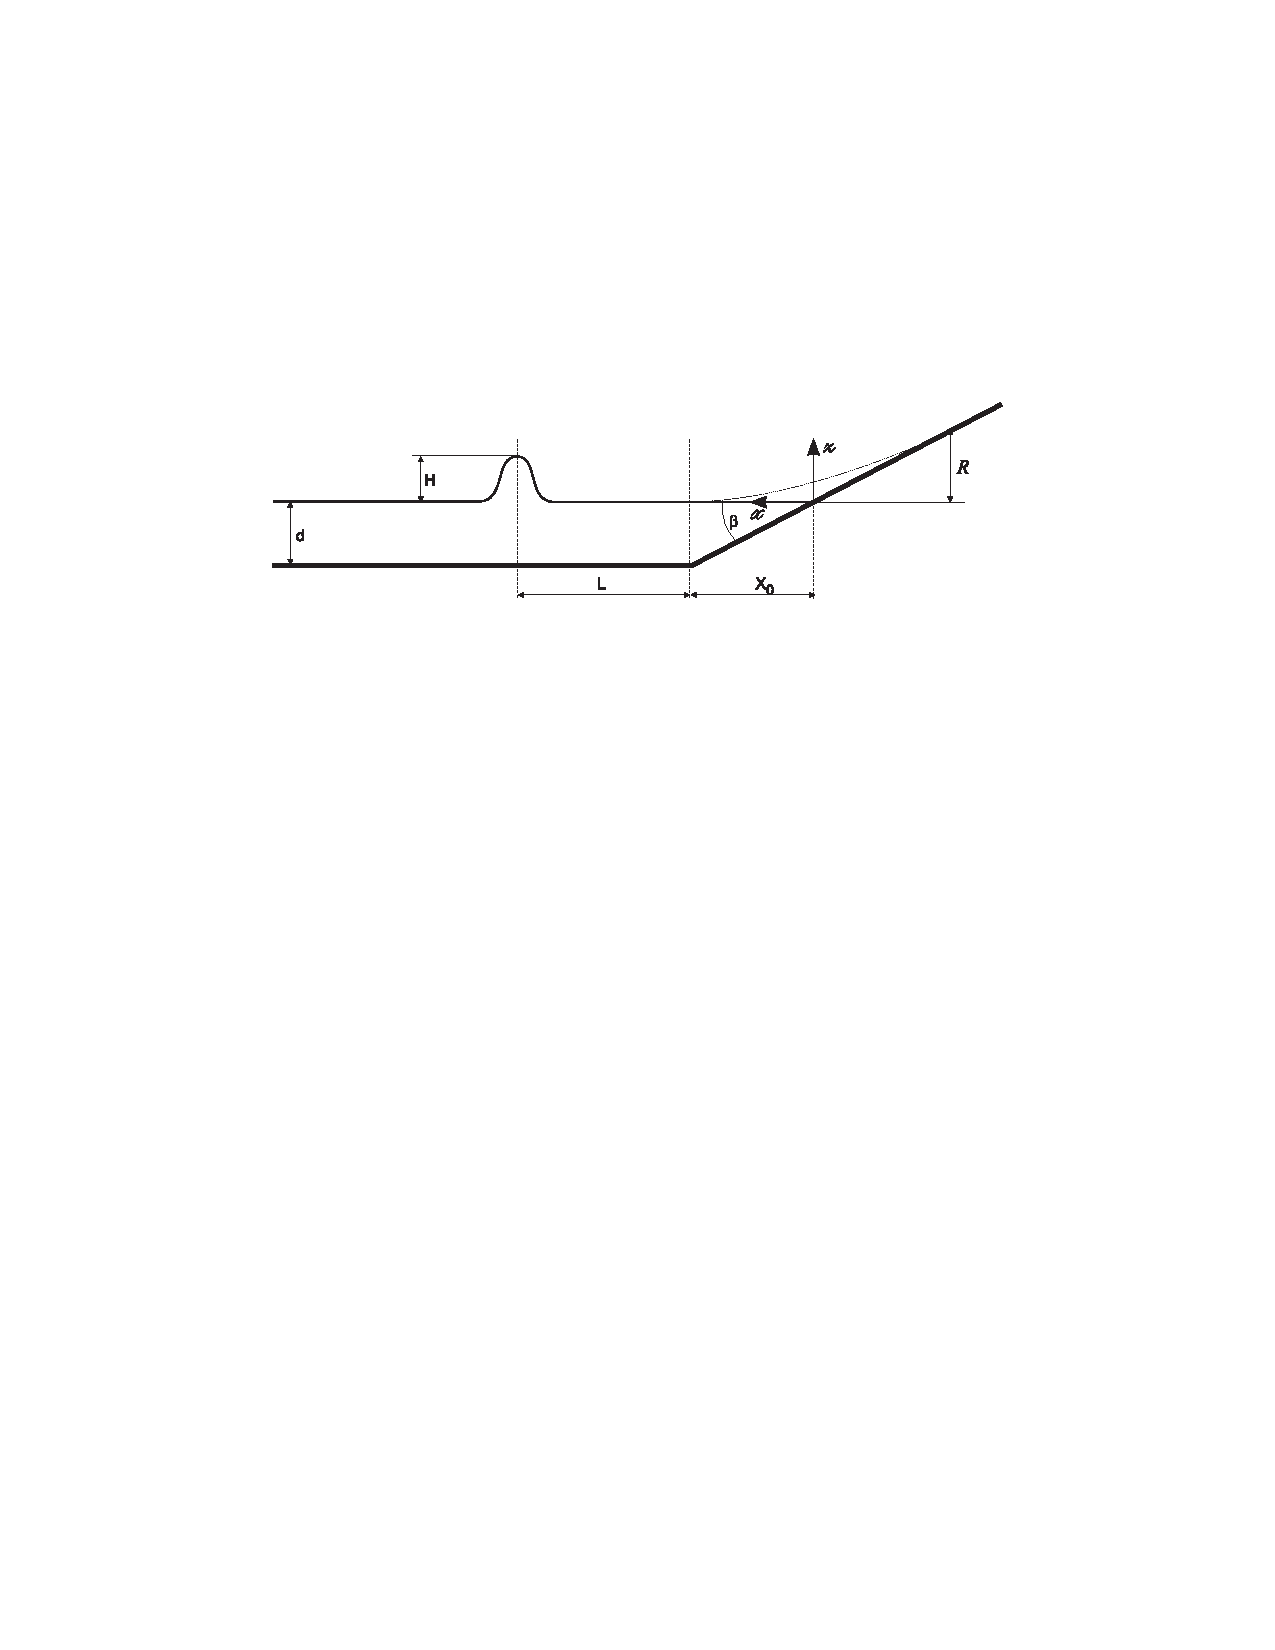
\includegraphics[width=5.0in]{bp1/bp1domain}\hfil
\caption{\label{fig:bp1domain} 
Sketch of canonical beach and approaching wave.
 }
\end{figure}


\subsubsection{Problems encountered}

\begin{itemize}
\item The analytic solution of the wave equation was hard to determine and compute.  The analytic solution was obtained from the benchmark problem champion; it would be very helpful if it were provided in an Excel file as part of the benchmark problem description.  
\item No analytical solution was provided for time $t = 25s$
\item The Clawpack code does not currently include maximum runup calculations. An additional module had to be written. 
\end{itemize}

\subsubsection{What we did}

\begin{itemize}
\item Used $g=1$ and no friction.
\item The problem was solved on an $800\times 2$ grid, where the x domain spanned x = -10 to 60.
\item Variable time stepping was allowed, based on a CFL number of 0.9
\end{itemize} 

\subsubsection{Results}
\begin{itemize}
\item Task 1. Good agreement between computed and analytic water level profiles at $t = 35(d/g)^{1/2}$, $t = 45(d/g)^{1/2}$, $t = 55(d/g)^{1/2}$, $t = 65(d/g)^{1/2}$ is presented in Figure \Fig{bp1frames}.  Data were missing from file {\tt canonical\_profiles.txt} for $t=25(d/g)^{1/2}$, so this time was omitted.
\item Task 2. Good agreement between computed and analytic water levels at locations $x/d = 0.25$ and $x/d = 9.95$ during the propagation and reflection of the wave is presented in Figure \Fig{bp1gauges}.
\item Task 3. Maximum runup on the beach was 0.085, as presented in the time series of runup values in Figure \Fig{bp1runup}.
\item Task 4. The optional demonstration of convergence was not performed.
\end{itemize}

\begin{figure}[ht]
\hfil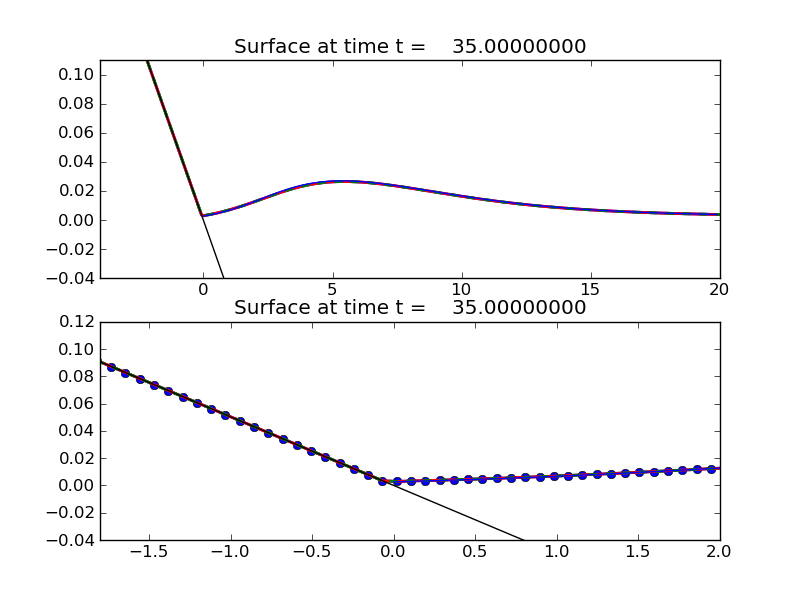
\includegraphics[width=2.8in]{bp1/frame0001fig2.png}\hfil
\hfil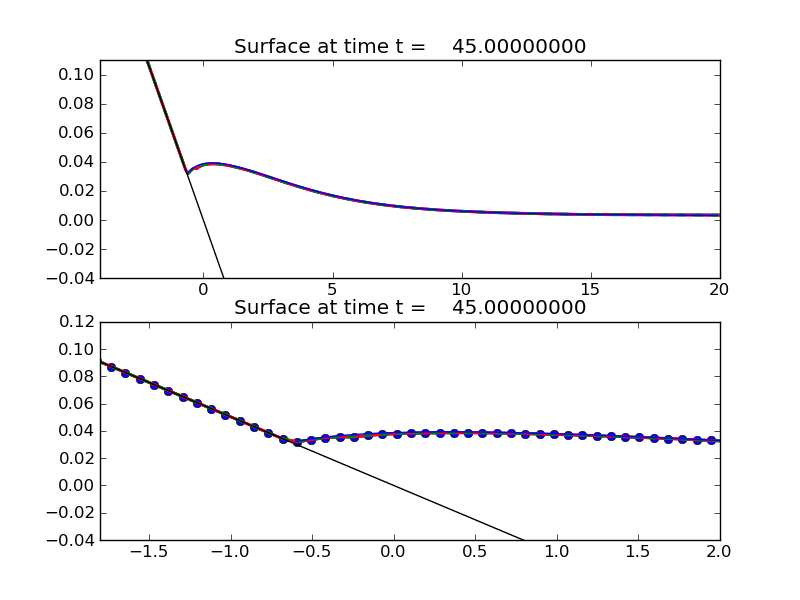
\includegraphics[width=2.8in]{bp1/frame0003fig2.png}\hfil
\vskip 5pt
\hfil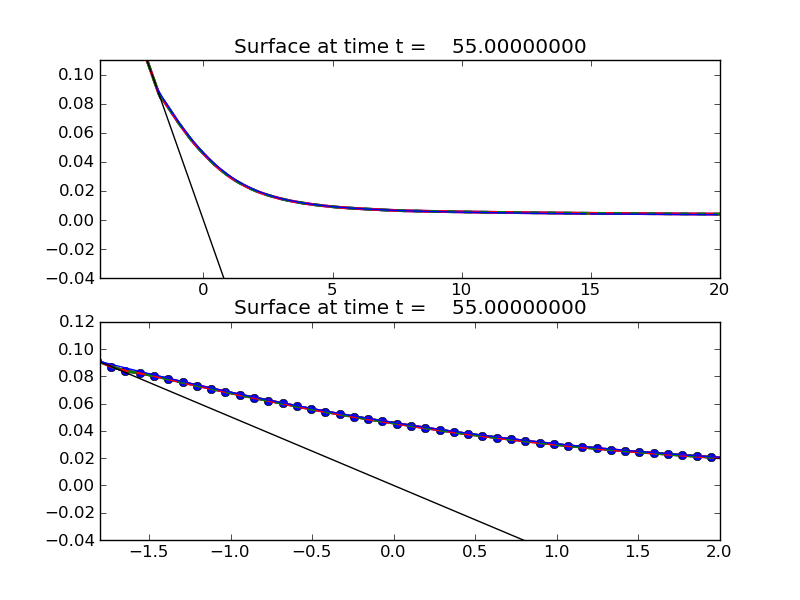
\includegraphics[width=2.8in]{bp1/frame0005fig2.png}\hfil
\hfil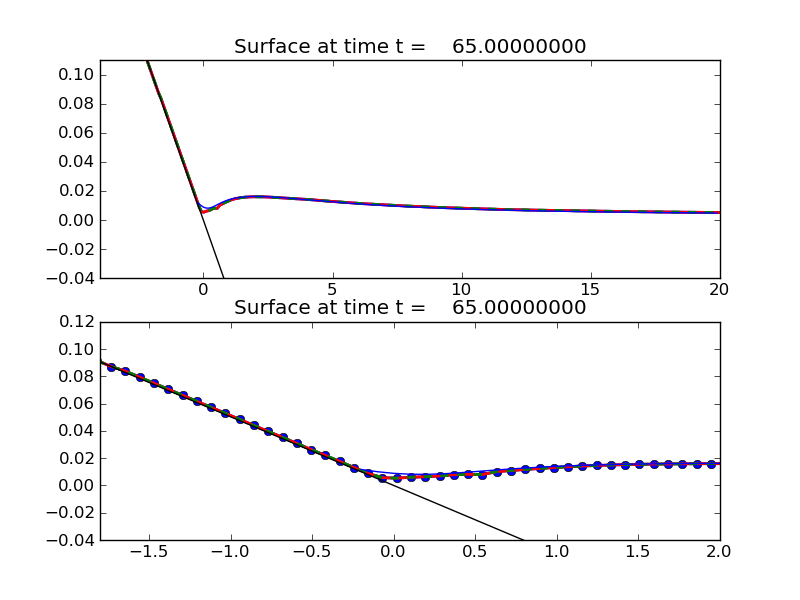
\includegraphics[width=2.8in]{bp1/frame0007fig2.png}\hfil
\caption{\label{fig:bp1frames} 
Profile plots for the times specified in Task 2.  For each pair of plots at a particular time, the top frame provides a full view of the incoming wave and the bottom frame provides an expanded view of the inundation area. In some regions the analytic and GeoClaw solutions lie atop one another.
\todo{Redo plots with only two lines?  Currently several curves are
all the same.}}
\end{figure}

\begin{figure}[ht]
\hfil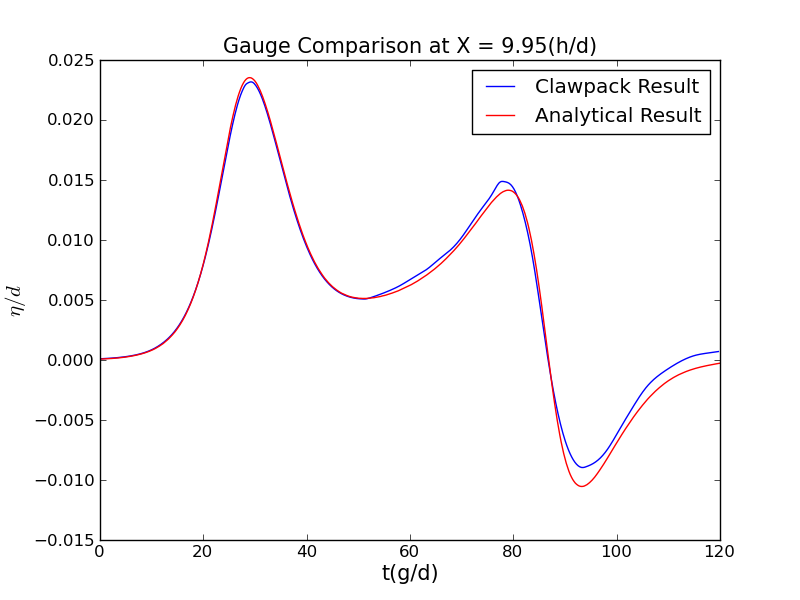
\includegraphics[width=2.8in]{bp1/plotgauge2.png}\hfil
\hfil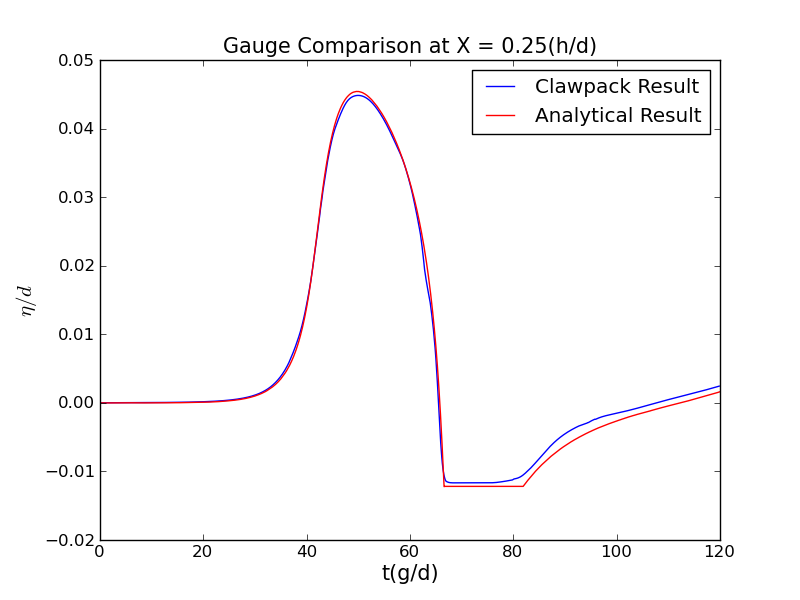
\includegraphics[width=2.8in]{bp1/plotgauge1.png}\hfil
\caption{\label{fig:bp1gauges} 
Left column: Water level time series at location $x/d = 9.95$.
Right column: Water level time series at location $x/d = 0.25$.
 }
\end{figure}

\begin{figure}[ht]
\hfil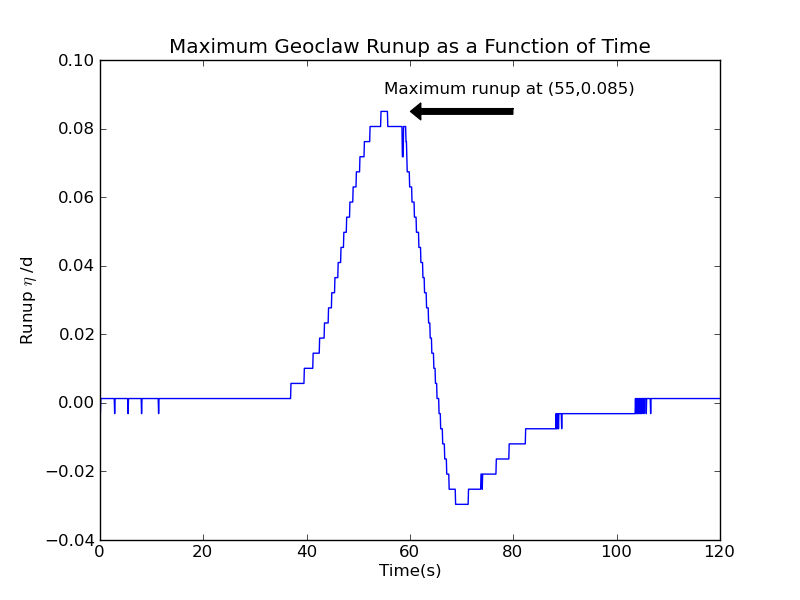
\includegraphics[width=5.5in]{bp1/runup.png}\hfil
\caption{\label{fig:bp1runup} 
Runup on canonical beach as a function of time}
\end{figure}

\subsubsection{Lessons learned}

\begin{itemize}
\item This benchmark problem is a good test of the shallow water wave computation against an analytic solution in one dimension.
\item Because of its complexity, the analytical solution should be provided in a data file on the benchmark problem website to ensure all participants are solving the same problem.
\end{itemize}

\newsection

\subsection{BP 2:
 Solitary wave on composite beach (Analytic)}

{\bf Documentation:}

\begin{itemize}
\item PMEL-135, pp 5 \& 30-33 \cite{SynolakisBernard:pmel135}.
\item Problem description \cite{bp-description}.
\item Coastal Hydraulics Laboratory Problem Description \cite{CHLBP2}.
\end{itemize}

\subsubsection{What we did}
\begin{itemize}

\item We solved the shallow water wave equation in Cartesian coordinates with $g = 9.81$ and no friction.
\item To specify the incoming wave from the left boundary of our computational domain we used the first ten seconds of  measurements taken at Gage 4.  After ten seconds the left boundary switched to be a non-reflecting boundary.  This boundary is selected since the end of our computational domain is not the end of the physical wave tank.  
The implementation of these boundary conditions is described in \Sec{bc}.
\item Since the problem is one-dimensional, we solved on a $600 \times 2$ grid with no adaptive mesh refinement.
\item To impose linearization we scaled the incoming wave by $10^{-4}$ to
remove  any nonlinear behavior, then scaled up the gage readings by $10^4$
to compare with the analytical solution.
\end{itemize}

\subsubsection{Gage comparisons}
For these Gage comparisons we ran our code linearly with friction set to zero. 

The results for cases A, B, and C are shown in figures \Fig{bp2A}, \Fig{bp2B}, \Fig{bp2C} respectively where Gage 11 is placed at the vertical wall.

\begin{figure}[ht]
\hfil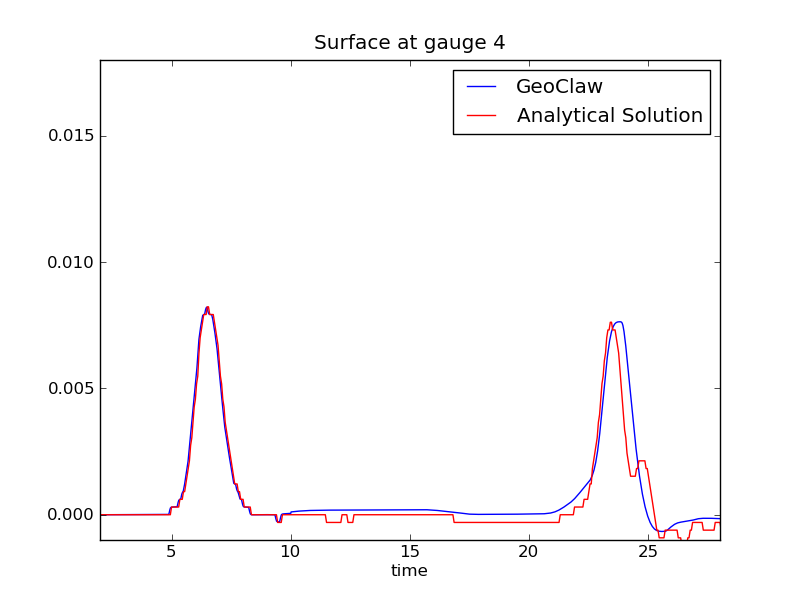
\includegraphics[width=2.8in]{bp2/CaseA/gauge0004fig300.png}\hfil
\hfil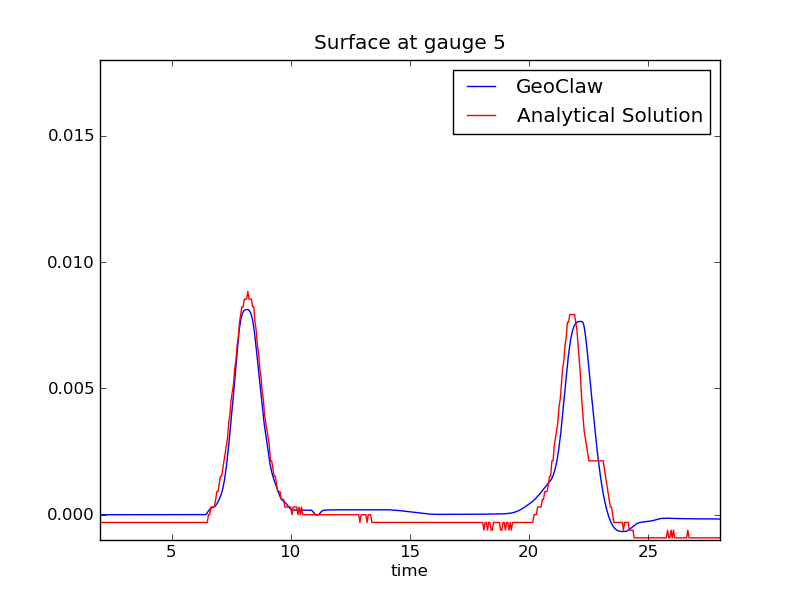
\includegraphics[width=2.8in]{bp2/CaseA/gauge0005fig300.png}\hfil
\vskip 5pt
\hfil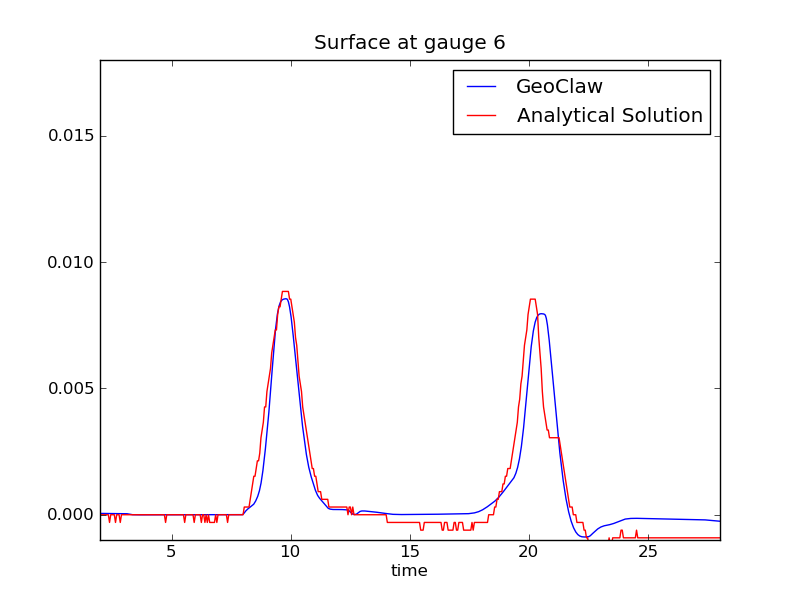
\includegraphics[width=2.8in]{bp2/CaseA/gauge0006fig300.png}\hfil
\hfil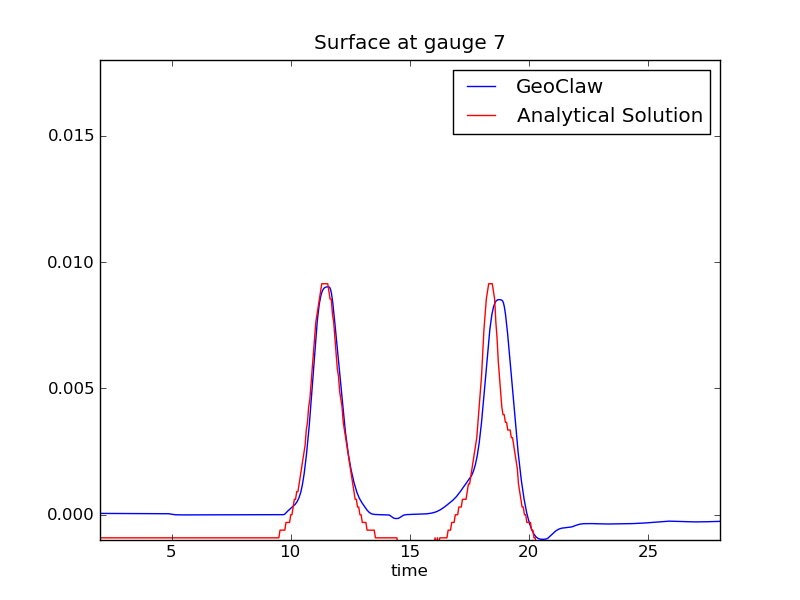
\includegraphics[width=2.8in]{bp2/CaseA/gauge0007fig300.png}\hfil
\vskip 5pt
\hfil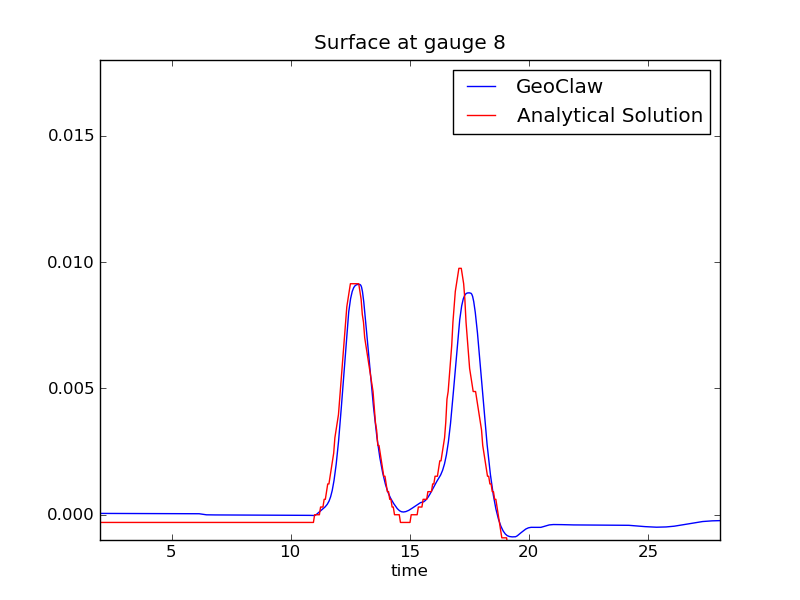
\includegraphics[width=2.8in]{bp2/CaseA/gauge0008fig300.png}\hfil
\hfil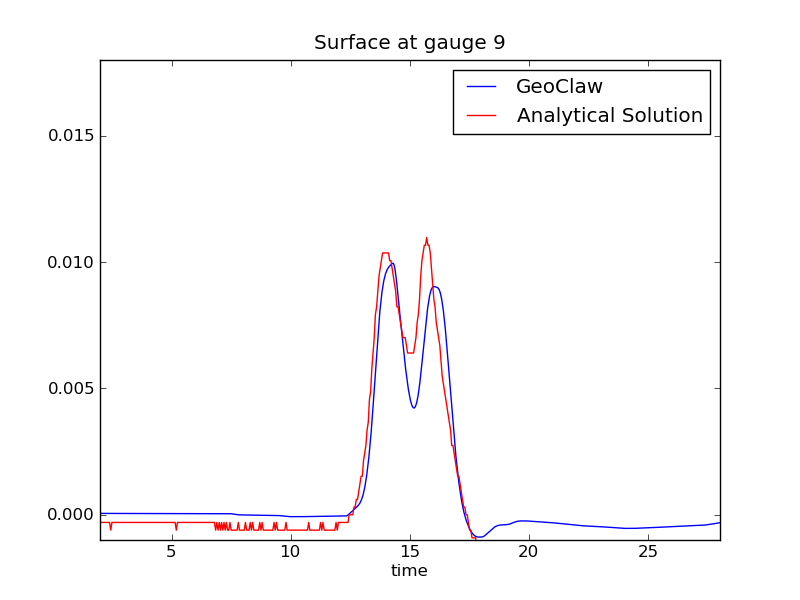
\includegraphics[width=2.8in]{bp2/CaseA/gauge0009fig300.png}\hfil
\vskip 5pt
\hfil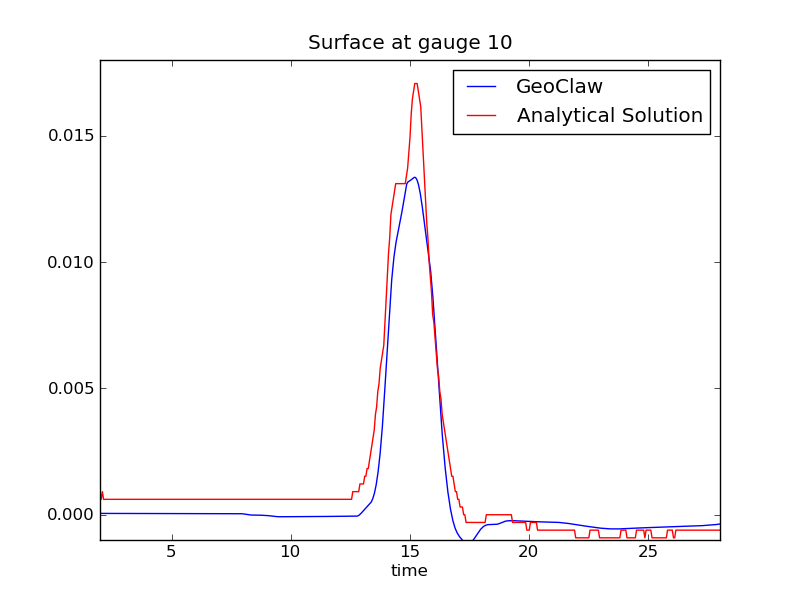
\includegraphics[width=2.8in]{bp2/CaseA/gauge0010fig300.png}\hfil
\hfil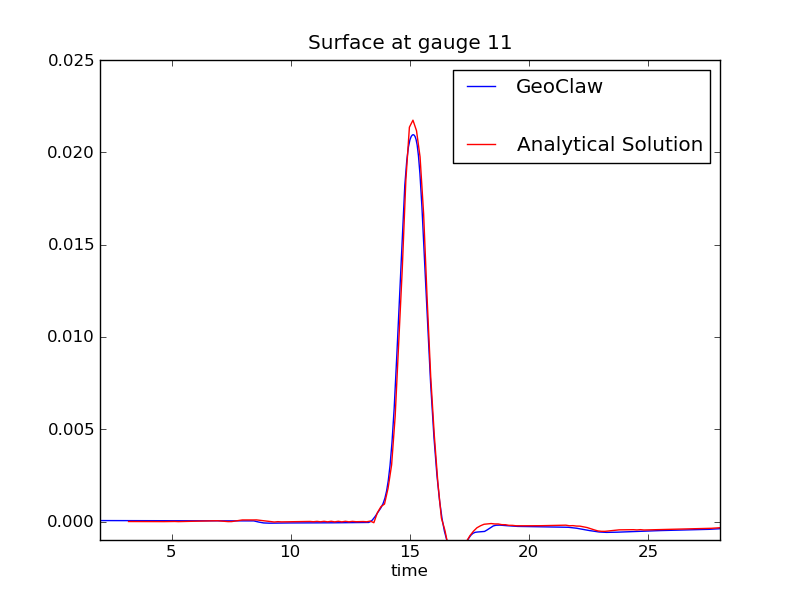
\includegraphics[width=2.8in]{bp2/CaseA/gauge0011fig300.png}\hfil
\caption{\label{fig:bp2A} Case A }
\end{figure}

\begin{figure}[ht]
\hfil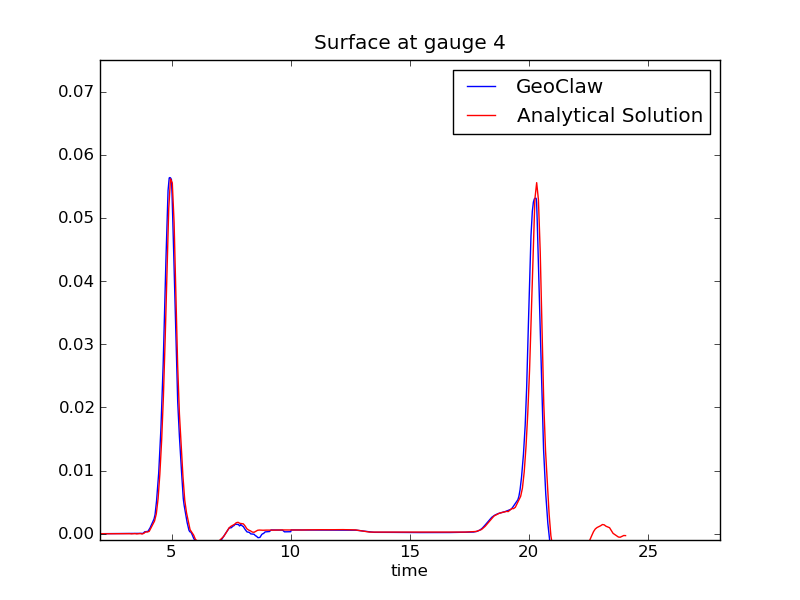
\includegraphics[width=2.8in]{bp2/CaseB/gauge0004fig300.png}\hfil
\hfil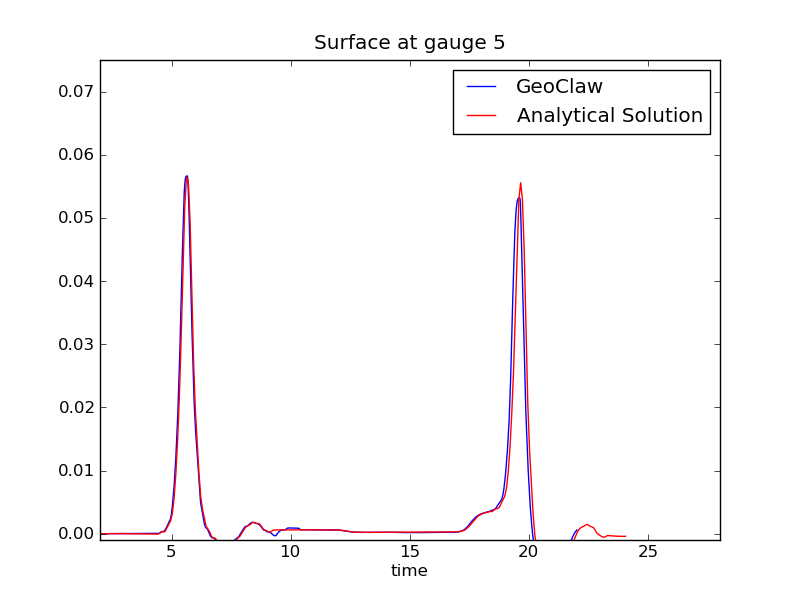
\includegraphics[width=2.8in]{bp2/CaseB/gauge0005fig300.png}\hfil
\vskip 5pt
\hfil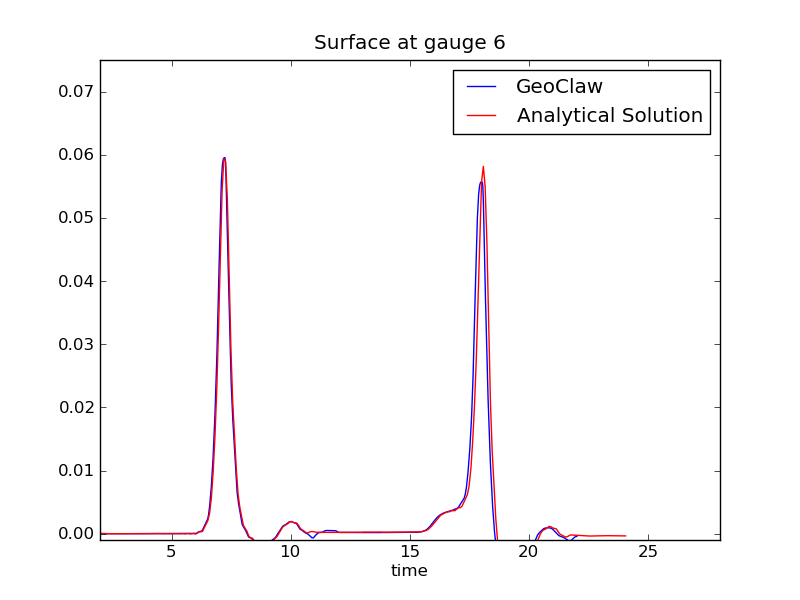
\includegraphics[width=2.8in]{bp2/CaseB/gauge0006fig300.png}\hfil
\hfil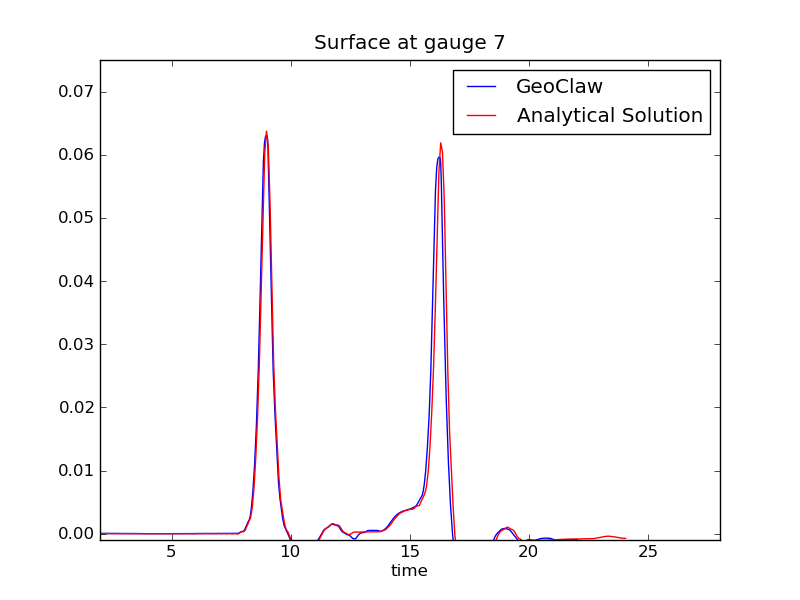
\includegraphics[width=2.8in]{bp2/CaseB/gauge0007fig300.png}\hfil
\vskip 5pt
\hfil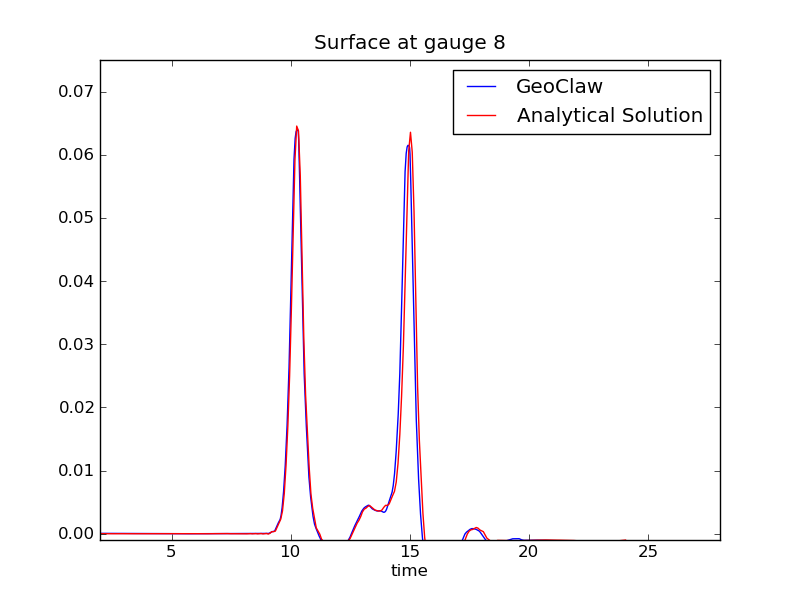
\includegraphics[width=2.8in]{bp2/CaseB/gauge0008fig300.png}\hfil
\hfil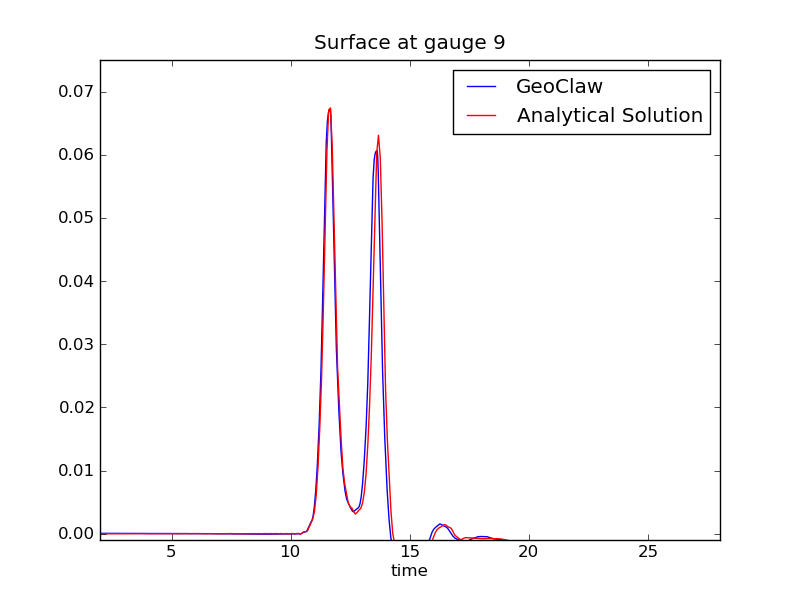
\includegraphics[width=2.8in]{bp2/CaseB/gauge0009fig300.png}\hfil
\vskip 5pt
\hfil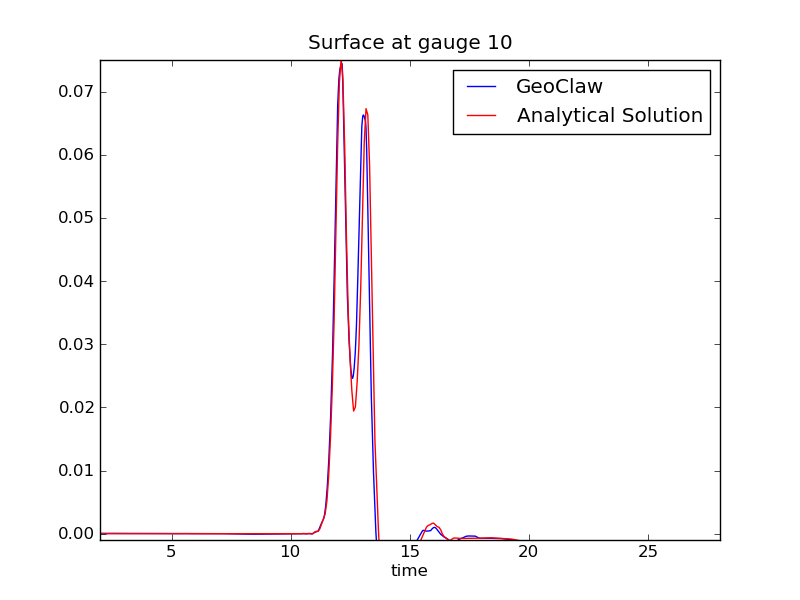
\includegraphics[width=2.8in]{bp2/CaseB/gauge0010fig300.png}\hfil
\hfil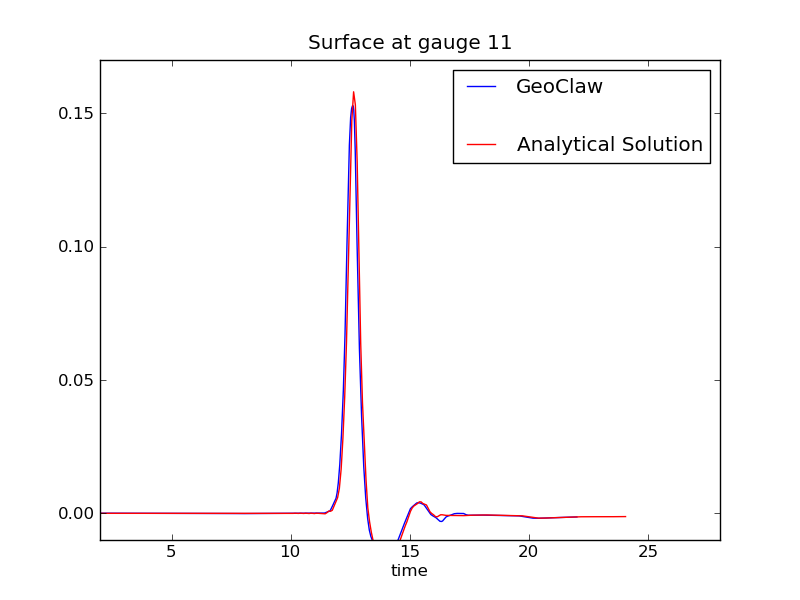
\includegraphics[width=2.8in]{bp2/CaseB/gauge0011fig300.png}\hfil
\caption{\label{fig:bp2B} Case B }
\end{figure}


\begin{figure}[ht]
\hfil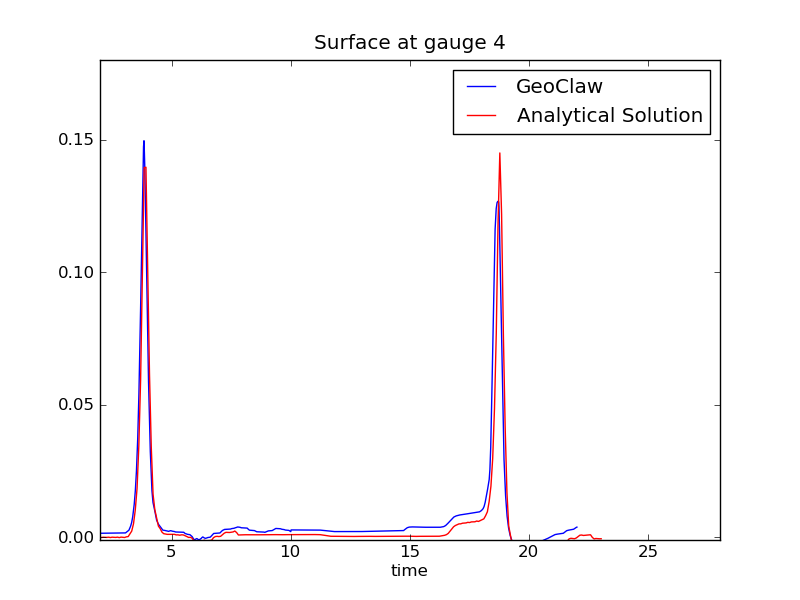
\includegraphics[width=2.8in]{bp2/CaseC/gauge0004fig300.png}\hfil
\hfil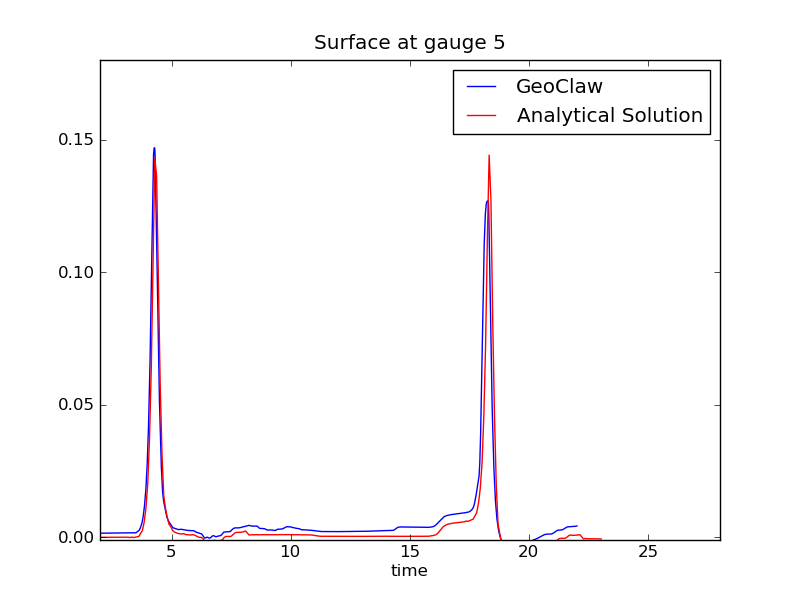
\includegraphics[width=2.8in]{bp2/CaseC/gauge0005fig300.png}\hfil
\vskip 5pt
\hfil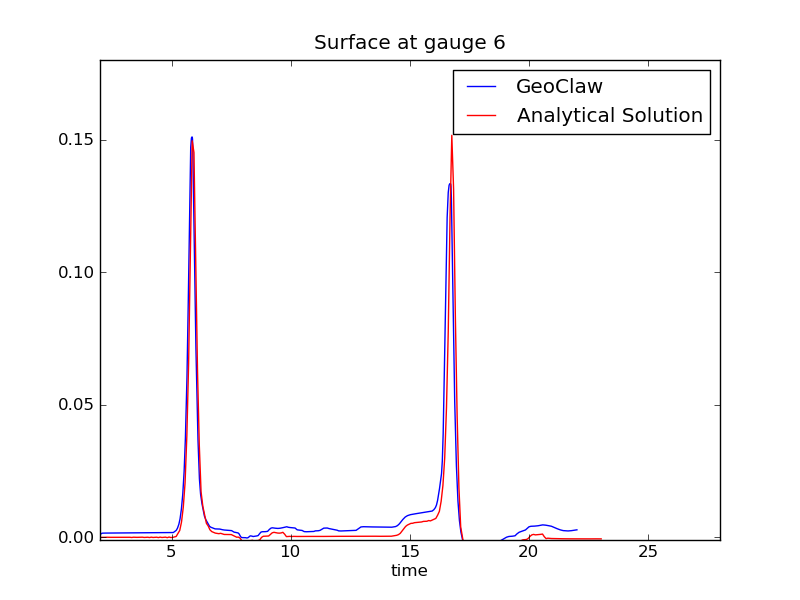
\includegraphics[width=2.8in]{bp2/CaseC/gauge0006fig300.png}\hfil
\hfil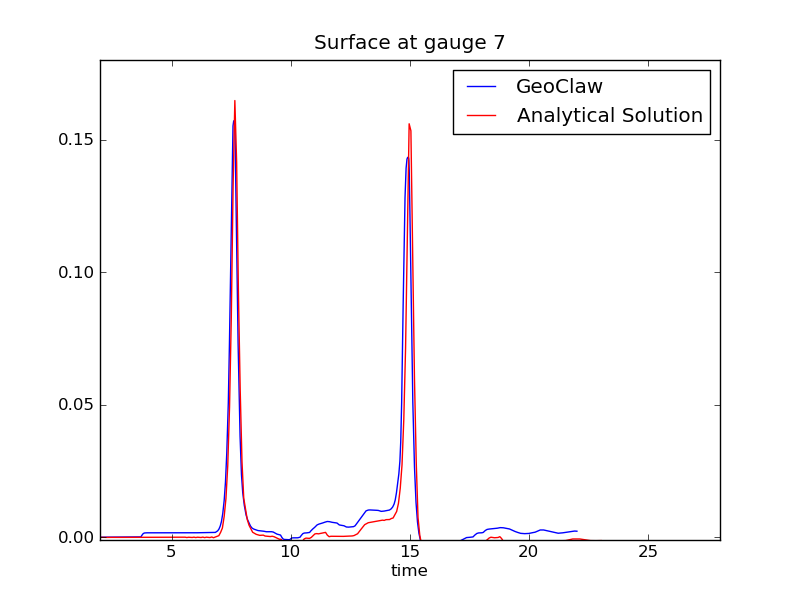
\includegraphics[width=2.8in]{bp2/CaseC/gauge0007fig300.png}\hfil
\vskip 5pt
\hfil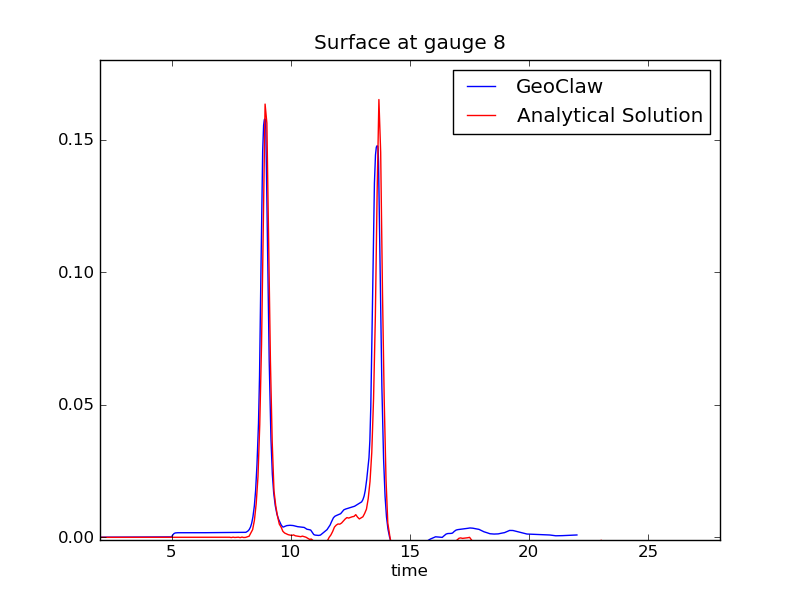
\includegraphics[width=2.8in]{bp2/CaseC/gauge0008fig300.png}\hfil
\hfil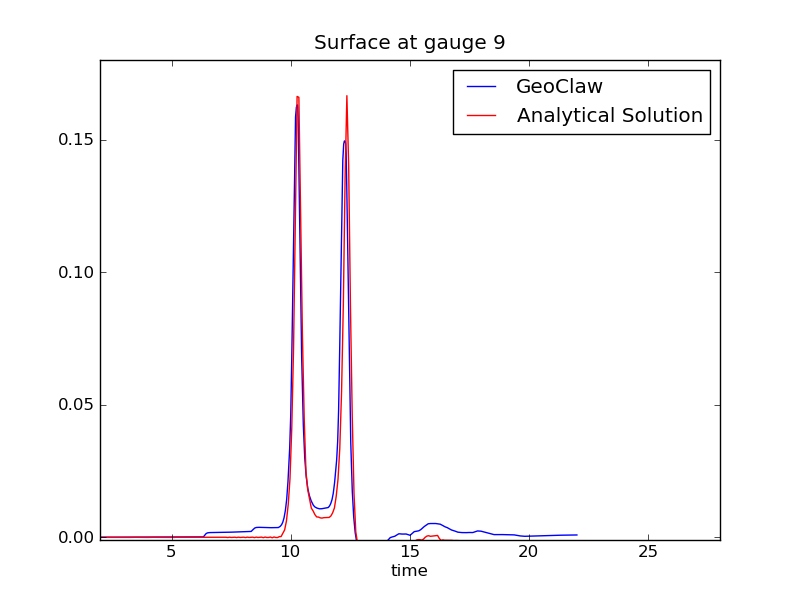
\includegraphics[width=2.8in]{bp2/CaseC/gauge0009fig300.png}\hfil
\vskip 5pt
\hfil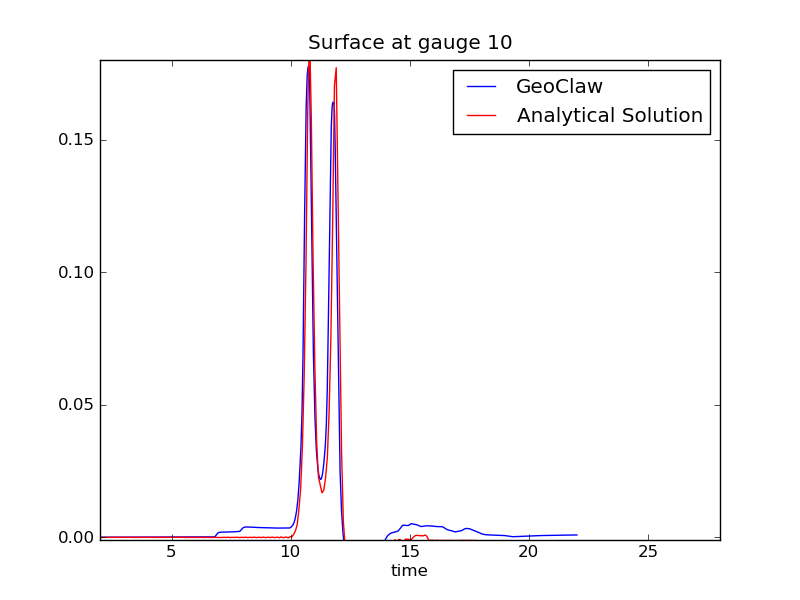
\includegraphics[width=2.8in]{bp2/CaseC/gauge0010fig300.png}\hfil
\hfil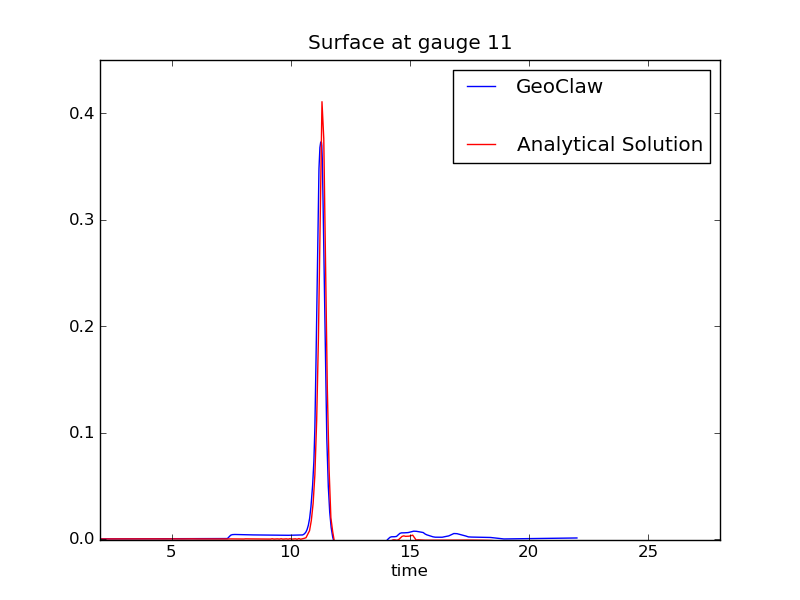
\includegraphics[width=2.8in]{bp2/CaseC/gauge0011fig300.png}\hfil
\caption{\label{fig:bp2C} Case C }
\end{figure}

\subsubsection{Convergence Study}
We performed a test to see how well Clawpack converged to the analytic
solution as we increased the number of grid cells in our computational
domain (using 200, 400, and 600 cells).  
We found that as the number of grid cells was increased,  the computed solution approached the analytic solution.  The convergence plot is shown in \Fig{linearConverge}.

\begin{figure}[ht]
\hfil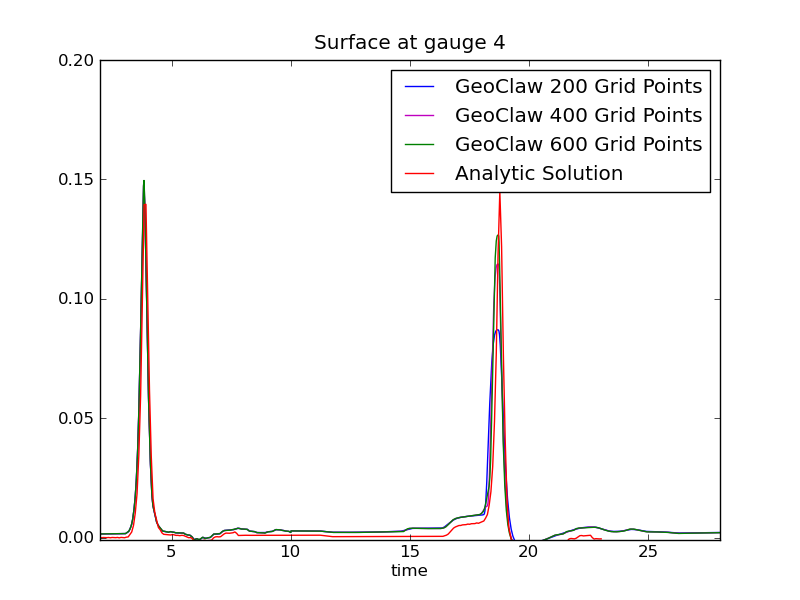
\includegraphics[width=5.8in]{bp2/linearCompare}\hfil
\caption{\label{fig:linearConverge} Convergence Plot for Gage 4 in Case C }
\end{figure}


\subsubsection{Lessons learned}
In this benchmark problem we found that using the analytic solution at Gage 4 as boundary conditions on a shorter domain, starting at gage 4, provided more accurate results than using the wave maker position and a longer domain to model the entire tank.  It appears that a similar assumption is made in the provided analytic solutions, as they match up nearly perfectly with the lab data for the first ten seconds.  

Overall this benchmark problem is a good test for one dimensional codes.  The benchmark problem specifications could be improved by specifying the computational domain and the specific data source that should be used to model the incoming wave. 


\newsection
\subsection{BP 3:    
 Saucer landslide (Laboratory)}

\subsubsection{Problem specification}

\begin{itemize}


\item Problem description provided by Stephan Grilli
      \cite{bp-description}.  %% fill in the problem number

\item Original paper of Enet and Grilli \cite{EnetGrilli}
describing laboratory experiments.

\end{itemize} 

\subsubsection{Problems encountered}

The moving bathymetry is specified in terms of $\zeta(\xi,\eta)$,
the thickness of the sliding mass 
in the direction orthogonal to the sloping beach.  In each time step this must
be converted into values $B(x,y,t)$ in the vertical $z$-direction, 
at horizontal distance $x$ from the initial shore.  Note that
\[
x = \xi \cos(\theta), \qquad y = \eta.
\]
The bathymetry of the wave tank and beach without the sliding mass is given by
\[
B_0(x,y) = \begin{pwdef} 
  -\tan(\theta)x \when x < 5.598, \\
  -1.5 \when x \geq 5.598 \end{pwdef}
\]
The value $5.598 \approx 1.5 / \tan(\theta)$ is determined by the fact that the
water has a depth of 1.5 m on the flat portion and the beach slope is
$15^\circ$ so $\theta = 15\pi/180 \approx 0.2618$.

At time $t=0$ the sliding mass is located at $x=x_0$, determined by the
initial depth $d$ according to
\[
x_0 = \frac{d}{\tan(\theta)} + \frac{T'}{\sin(\theta)}.
\]

At time $t$ the sliding mass is centered at $x_c = x_0 + s(t)\cos(\theta)$
where $s(t)$ is the function discretized in the data file
{\tt kinematics.txt}.    However, this is only true for small $t$.  After
some time the mass hits the horizontal bottom of the tank.  According the
paper \cite{EnetGrilli} and communication with Stephan Grilli, the mass stops at
this point.  This is not made clear in the problem specification 
\cite{bp-description}.


To determine $B(x,y,t)$, for each finite volume grid cell with center 
$(x_i, y_j)$ the value $\xi$ must be found so that
\[
\xi\cos(\theta) + \zeta(\xi - \xi_c,y_j)\sin(\theta) = x_i
\]
where $\xi_c = x_0/\cos(\theta) + s(t)$  is the $\xi$ location of the center
of mass at this time.
Determining $\xi$ requires solving the nonlinear equation
\[
\cos(\theta)\xi + \zeta(\xi - \xi_c, y_j) \sin(\theta) - x_i = 0.
\]
In our Fortran code this equation is solved using the library routine {\tt
zeroin} available from Netlib (\url{http://www.netlib.org/go/zeroin.f}).

Once $\xi$ has been found, the bathymetry is 
\[
B(x_i,y_j,t) =
-\tan(\theta)\xi + \cos(\theta)\zeta(\xi - \xi_c, y_j).
\]


\subsubsection{What we did}\label{sec:bp3what}

%% Itemize the assumptions we made, etc.

\begin{itemize}
\item  The moving bathymetry is handled by recomputing $B_{ij}^n =
B(x_i,y_j,t_n)$ in
each time step, at the center of each finite volume grid cell, by solving a
nonlinear equation as described above.  This is the standard approach
for handling moving bathymetry in GeoClaw:  the value $B_{ij}^n$ is adjusted
but the fluid depth $h_{ij}^n$ remains the same, so that the water column is
simply displaced vertically in any cell where the bathymetry changes.  For
bathymetry that is smoothly varying  in space and time, as in this problem,
this is considered a reasonable approach.  Note, however, that no momentum
is directly imparted to the water by the moving bathymetry.  

\item The problem was solved using a fixed grid with $72n \times 18n$ grid
cells on the domain $-1\leq x \leq 6.2$ and $0\leq y \leq 1.8$ meters.
Three resolutions corresponding to $n=1,~2,~4$ were used to test
convergence.

A second level of refined grid was used in the region $-0.1\leq x \leq 0.1$
and $0\leq y \leq 0.1$ surrounding the point $x\approx 0, y=0$
on the shoreline where the runup $R_u$ must be calculated.  In each case
this grid was 10 times finer in each direction than the base grid.  

Adaptive mesh refinement (with moving grids) was not used.

\item The problem was solved on $0\leq y \leq 1.8$ with solid wall boundary
conditions at $y=0$.  This gives the correct solution in this
domain and the solution in the other half of the wave tank $-1.8\leq y\leq
0$  is easily constructed by symmetry if desired.

Solid wall boundary conditions were also used at $y=1.8$.  At $x=-1$ the
boundary condition doesn't matter since this region is always dry, and at
$x=6.2$ outflow boundary conditions were used.  Zero-order extrapolation,
which generally gives a very good approximation to non-reflecting boundary
conditions as described in Section 7.3.1 of \cite{rjl:fvmhp}.  Solid wall
boundary conditions are implemented as described in Section 7.3.3 of
\cite{rjl:fvmhp}.


\end{itemize} 


\subsubsection{Numerical simulations}

\Fig{bp3eta} shows two frames from
a sample computation for the case $d=0.061$. Colors indicate the surface
elevation $\eta(x,y,t)$ and contours show the bathymetry with the upper half
of the sliding mass.  


\begin{figure}[ht]

\hfil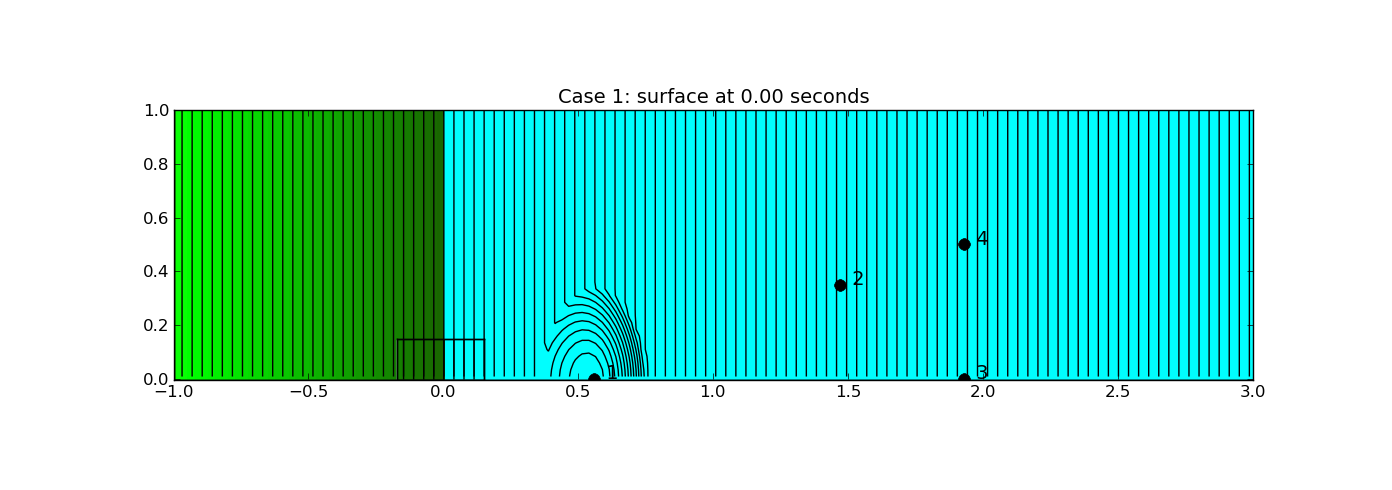
\includegraphics[width=5.8in]{bp3/frame0.png}\hfil
\vskip 10pt
\hfil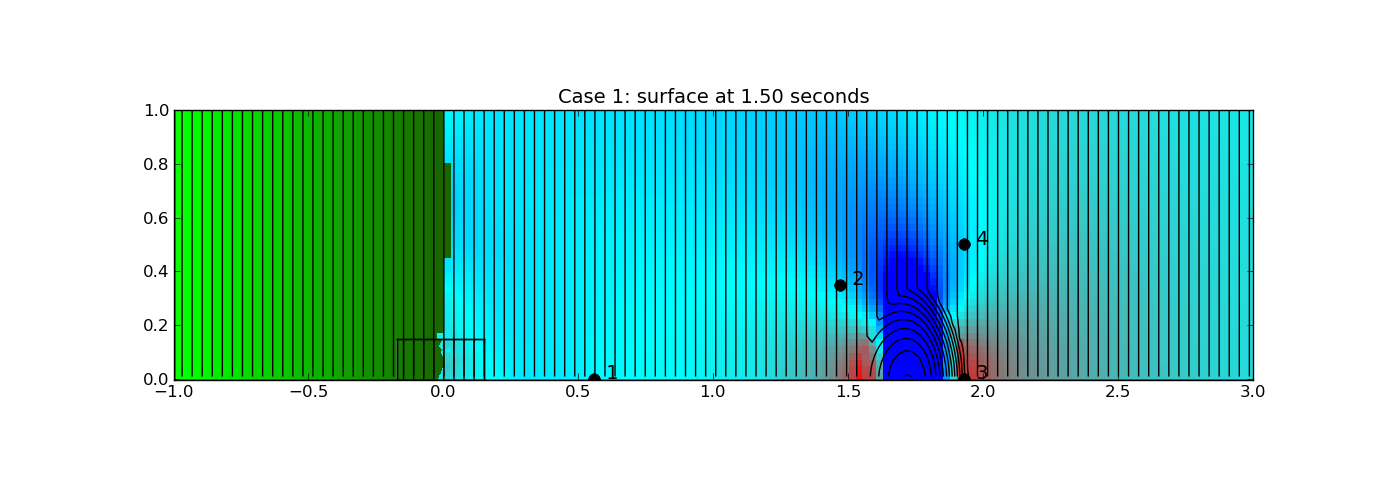
\includegraphics[width=5.8in]{bp3/frame6.png}\hfil

\caption{\label{fig:bp3eta} 
Sample results for $d=0.061$.  The water surface $\eta(x,y,t)$
(colors with dark red $+0.02$ m and dark blue $-0.02$ m) and bathymetry
(0.01 m contour levels).
Only a portion of the computational domain is shown.
Grid resolution: $\Delta x = \Delta y = 0.025$ m on the full domain,
with refinement to $\Delta x = \Delta y = 0.0025$ m 
in the nearshore region in the
the rectangular box.  The full domain goes to $x = 6.2$ and to $y=1.8$.
  }
\end{figure}



\subsubsection{Gauge comparisons}

Simulated gauges were placed at the 4 locations that match the wave tank
measurements, as indicated in \Fig{bp3eta}.
The surface elevation $\eta(t)$ at each gauge was recorded every time step.
These results are shown in Figures \ref{fig:bp3gauge1} through \ref{fig:bp3gauge7}
for the 7 test cases.

Reasonable agreement is generally seen for the initial peak and trough at 
Gauges 1, 2, and 4.  On the other hand 
Gauge 3, located along the centerline, shows quite
different results than the measurements and generally exhibits a steeper dip
in $\eta$ as the mass passes this point.   The measurements also show an
oscillatory wave train behind the initial peak and trough that is not
captured in the simulations obtained with the shallow water equations.  This
is consistent with claims in \cite{bp-description} and \cite{EnetGrilli}
that dispersive effects are important for these short wavelength waves that
cannot be captured by the non-dispersive shallow water equations.  By
contrast, the Boussinesq model used in \cite{??} does display these
dispersive ripples.




\begin{figure}[ht]

\hfil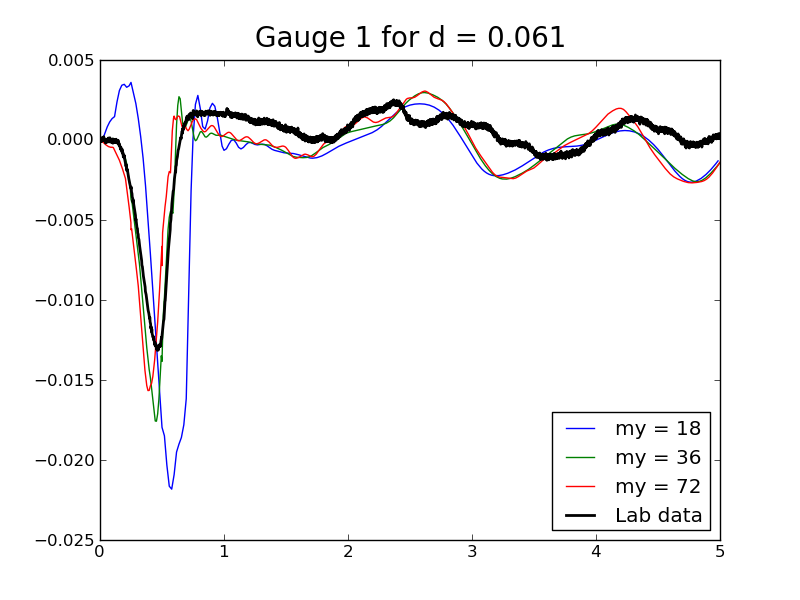
\includegraphics[width=2.8in]{bp3/gauge1-d0-061.png}\hfil
\hfil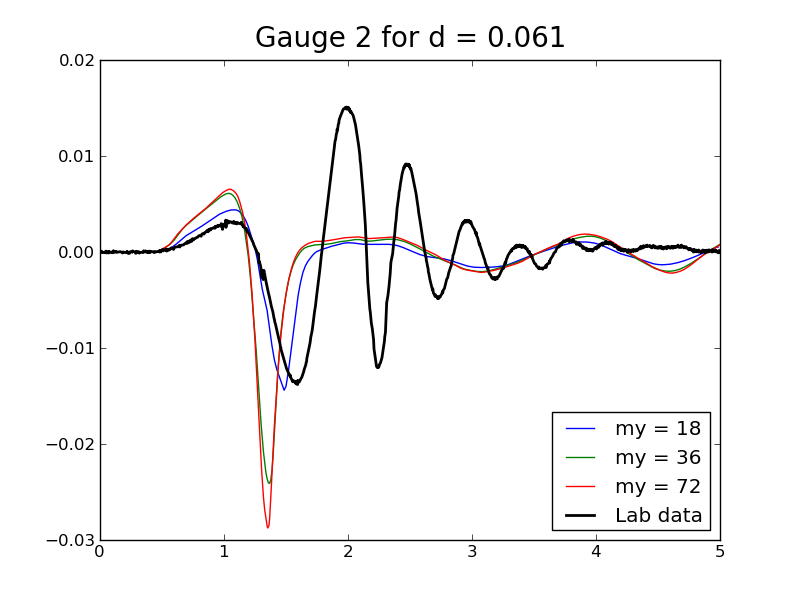
\includegraphics[width=2.8in]{bp3/gauge2-d0-061.png}\hfil
\vskip 10pt
\hfil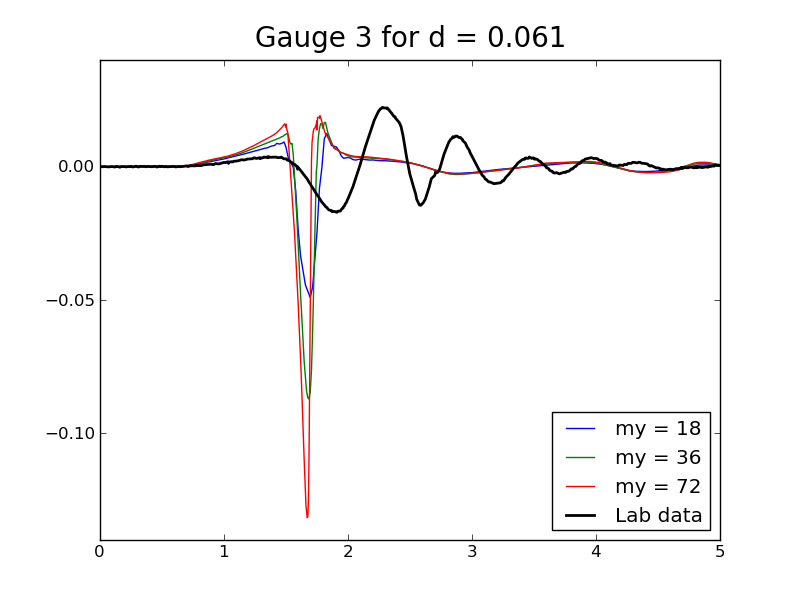
\includegraphics[width=2.8in]{bp3/gauge3-d0-061.png}\hfil
\hfil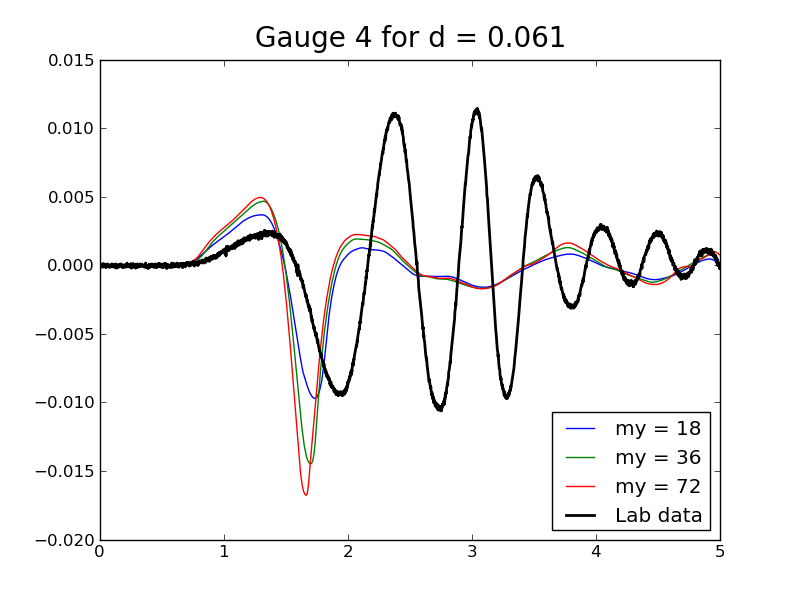
\includegraphics[width=2.8in]{bp3/gauge4-d0-061.png}\hfil
\vskip 10pt
\hfil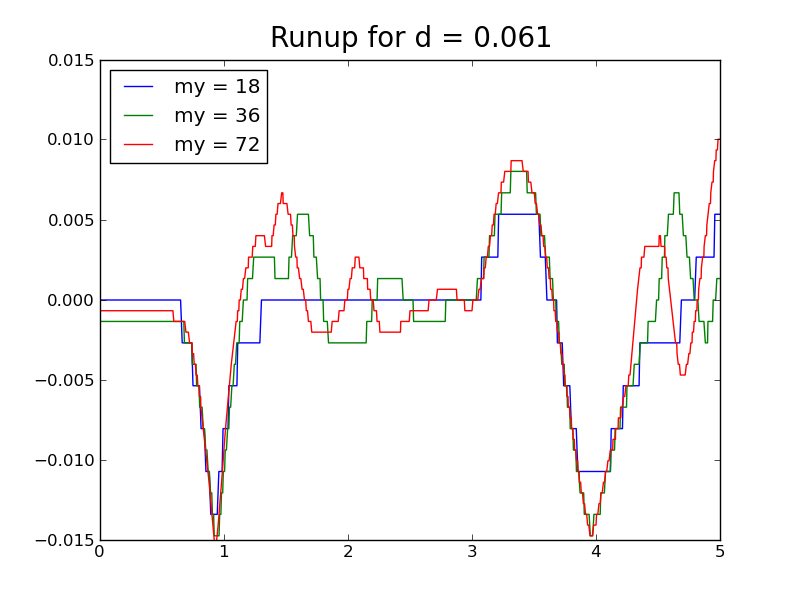
\includegraphics[width=2.8in]{bp3/runup-d0-061.png}\hfil

\caption{\label{fig:bp3gauge1} 
Gauge and runup results for $d=0.061$.
  }
\end{figure}


\begin{figure}[ht]

\hfil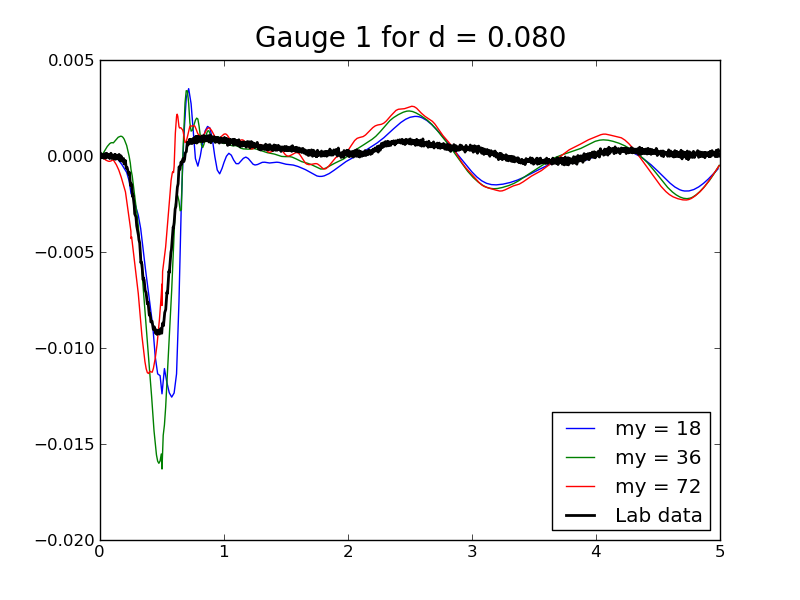
\includegraphics[width=2.8in]{bp3/gauge1-d0-08.png}\hfil
\hfil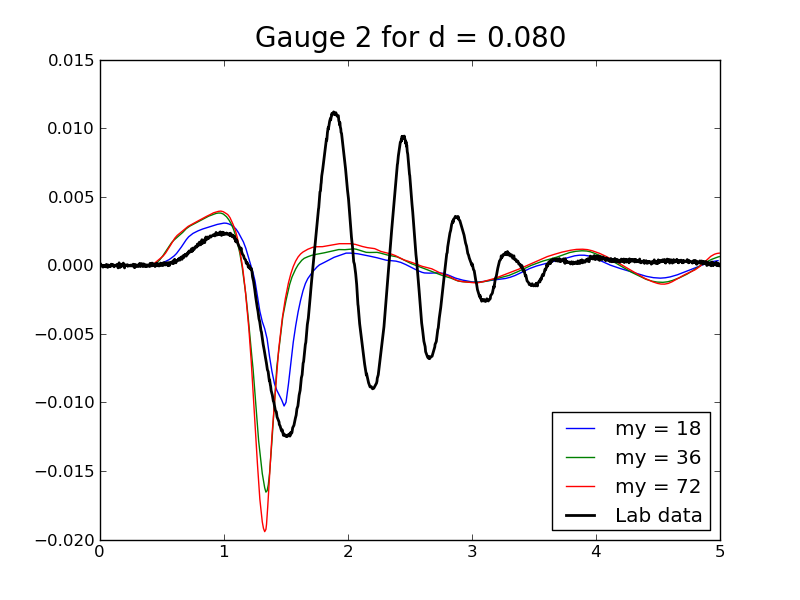
\includegraphics[width=2.8in]{bp3/gauge2-d0-08.png}\hfil
\vskip 10pt
\hfil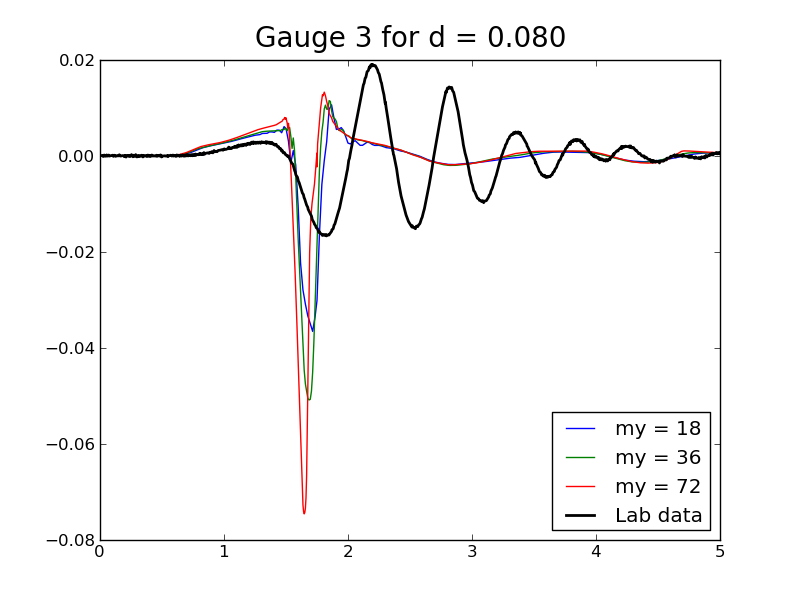
\includegraphics[width=2.8in]{bp3/gauge3-d0-08.png}\hfil
\hfil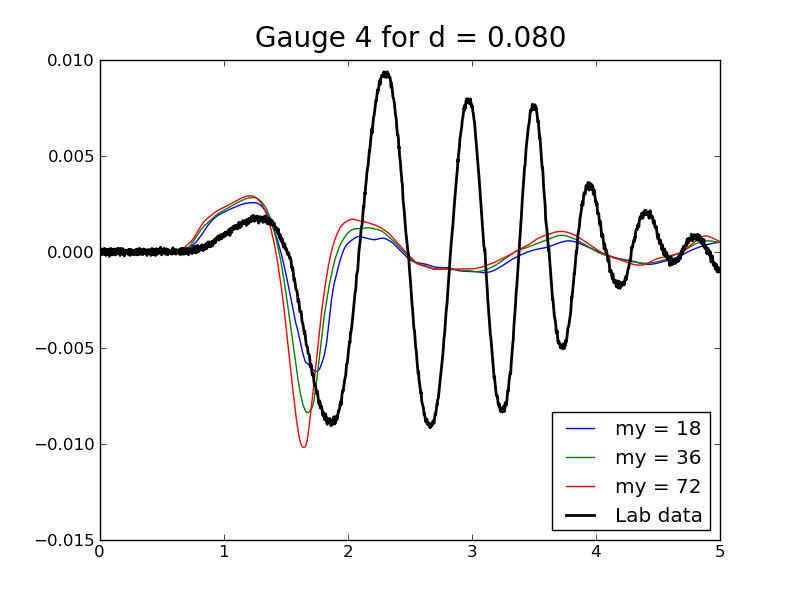
\includegraphics[width=2.8in]{bp3/gauge4-d0-08.png}\hfil
\vskip 10pt
\hfil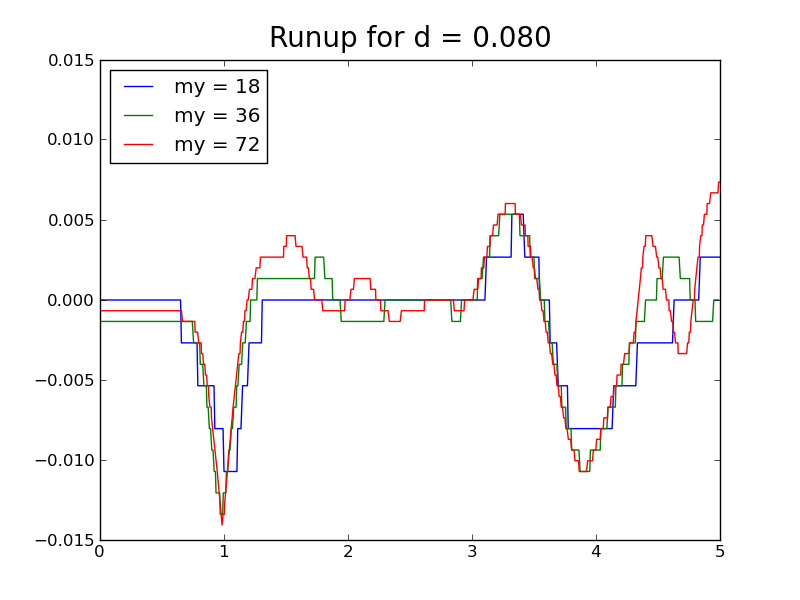
\includegraphics[width=2.8in]{bp3/runup-d0-08.png}\hfil

\caption{\label{fig:bp3gauge2} 
Gauge and runup results for $d=0.08$.
  }
\end{figure}



\begin{figure}[ht]

\hfil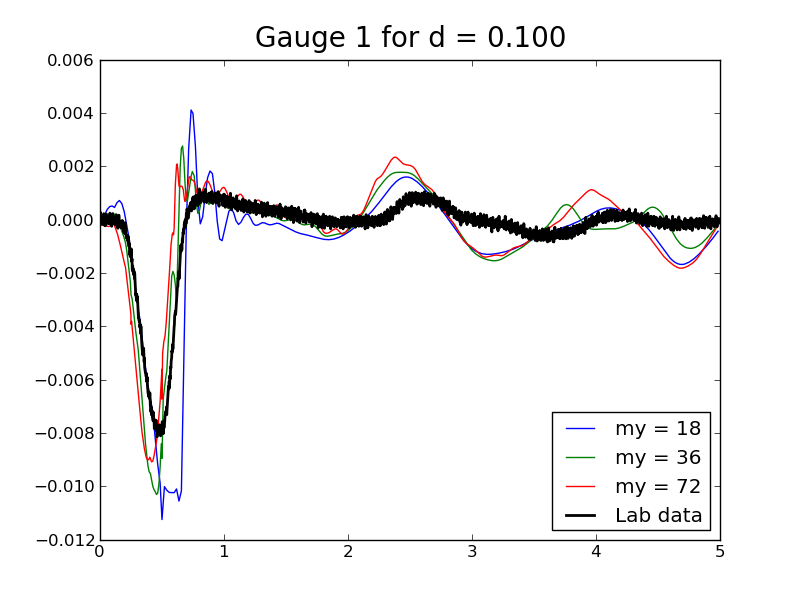
\includegraphics[width=2.8in]{bp3/gauge1-d0-1.png}\hfil
\hfil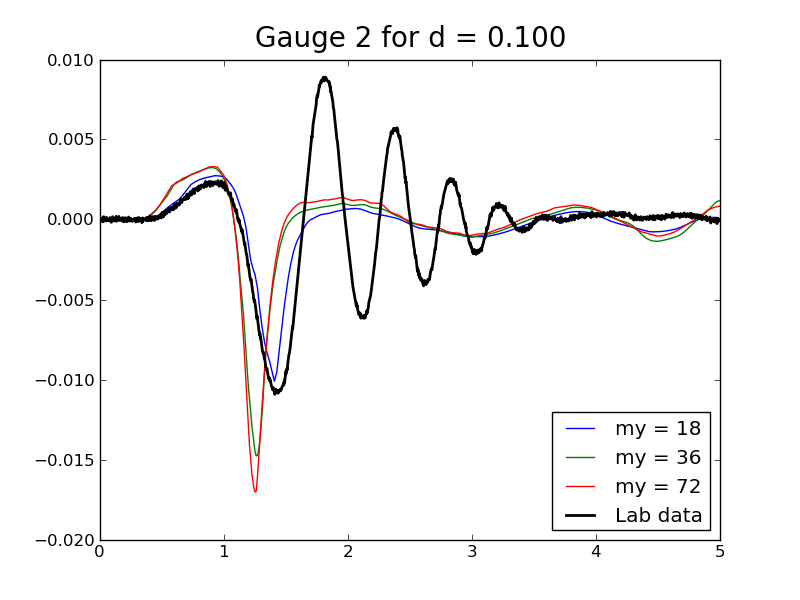
\includegraphics[width=2.8in]{bp3/gauge2-d0-1.png}\hfil
\vskip 10pt
\hfil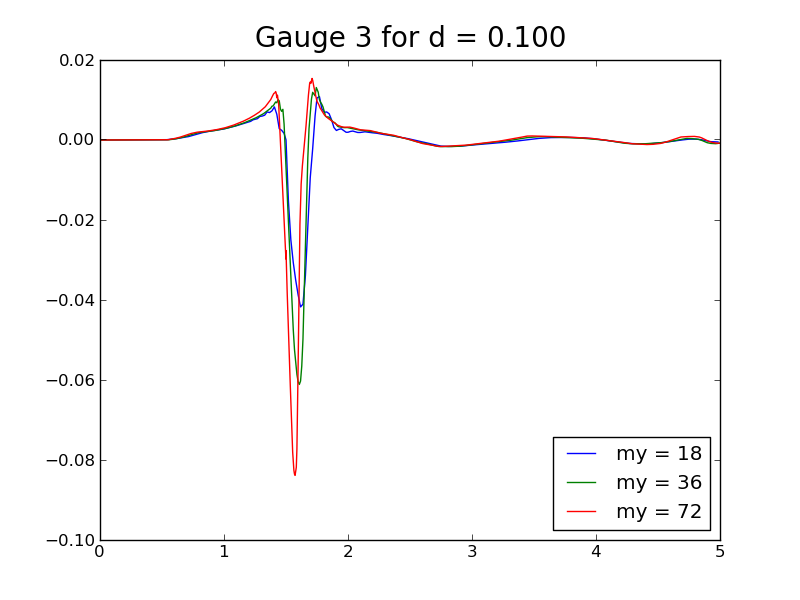
\includegraphics[width=2.8in]{bp3/gauge3-d0-1.png}\hfil
\hfil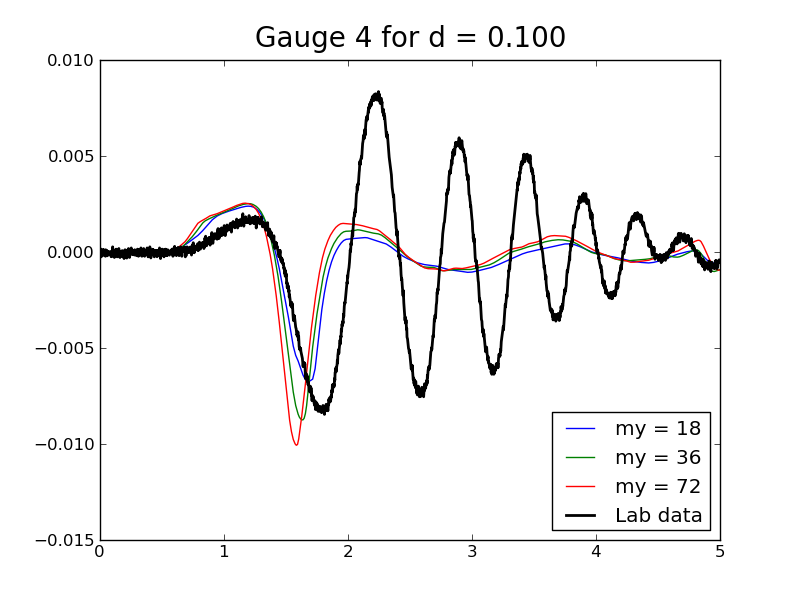
\includegraphics[width=2.8in]{bp3/gauge4-d0-1.png}\hfil
\vskip 10pt
\hfil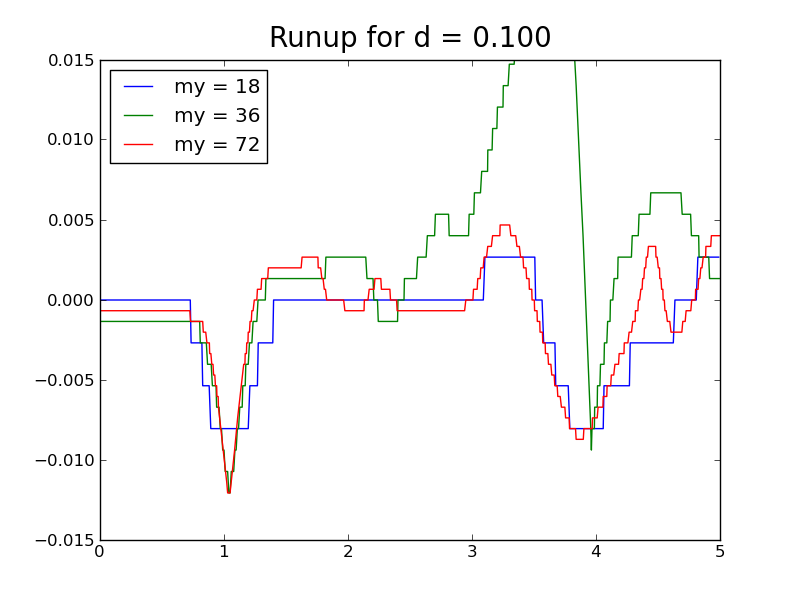
\includegraphics[width=2.8in]{bp3/runup-d0-1.png}\hfil

\caption{\label{fig:bp3gauge3} 
Gauge and runup results for $d=0.1$.
  }
\end{figure}



\begin{figure}[ht]

\hfil\includegraphics[width=2.8in]{bp3/gauge1-d0-12.png}\hfil
\hfil\includegraphics[width=2.8in]{bp3/gauge2-d0-12.png}\hfil
\vskip 10pt
\hfil\includegraphics[width=2.8in]{bp3/gauge3-d0-12.png}\hfil
\hfil\includegraphics[width=2.8in]{bp3/gauge4-d0-12.png}\hfil
\vskip 10pt
\hfil\includegraphics[width=2.8in]{bp3/runup-d0-12.png}\hfil

\caption{\label{fig:bp3gauge4} 
Gauge and runup results for $d=0.12$.
  }
\end{figure}



\begin{figure}[ht]

\hfil\includegraphics[width=2.8in]{bp3/gauge1-d0-14.png}\hfil
\hfil\includegraphics[width=2.8in]{bp3/gauge2-d0-14.png}\hfil
\vskip 10pt
\hfil\includegraphics[width=2.8in]{bp3/gauge3-d0-14.png}\hfil
\hfil\includegraphics[width=2.8in]{bp3/gauge4-d0-14.png}\hfil
\vskip 10pt
\hfil\includegraphics[width=2.8in]{bp3/runup-d0-14.png}\hfil

\caption{\label{fig:bp3gauge5} 
Gauge and runup results for $d=0.14$.
  }
\end{figure}



\begin{figure}[ht]

\hfil\includegraphics[width=2.8in]{bp3/gauge1-d0-149.png}\hfil
\hfil\includegraphics[width=2.8in]{bp3/gauge2-d0-149.png}\hfil
\vskip 10pt
\hfil\includegraphics[width=2.8in]{bp3/gauge3-d0-149.png}\hfil
\hfil\includegraphics[width=2.8in]{bp3/gauge4-d0-149.png}\hfil
\vskip 10pt
\hfil\includegraphics[width=2.8in]{bp3/runup-d0-149.png}\hfil

\caption{\label{fig:bp3gauge6} 
Gauge and runup results for $d=0.149$.
  }
\end{figure}



\begin{figure}[ht]

\hfil\includegraphics[width=2.8in]{bp3/gauge1-d0-189.png}\hfil
\hfil\includegraphics[width=2.8in]{bp3/gauge2-d0-189.png}\hfil
\vskip 10pt
\hfil\includegraphics[width=2.8in]{bp3/gauge3-d0-189.png}\hfil
\hfil\includegraphics[width=2.8in]{bp3/gauge4-d0-189.png}\hfil
\vskip 10pt
\hfil\includegraphics[width=2.8in]{bp3/runup-d0-189.png}\hfil

\caption{\label{fig:bp3gauge7} 
Gauge and runup results for $d=0.189$.
  }
\end{figure}



\subsubsection{Runup measurements}

The runup is measured near $y=0$ by keeping track of the approximate shoreline
position in the first row of grid cells $j=1$, whose centers lie at
$y=\Delta y / 2$.  In each time step, we loop over all cells
$i=1,~2,~\ldots$ and look for the first cell for which $h_{ij} > \epsilon$,
where $\epsilon = 0.001$ (1 mm) was chosen as a depth below which the cell
is considered dry.  
The value $x_s = i\Delta x$, the right edge of this finite volume cell, was
then used as the shoreline location at this time.  The runup at each time
is then computed as $x_s\tan(\theta)$, and this value was output for
later plotting, and for computing the maximum runup $R_u$ required for the
benchmark.

Figures \ref{fig:bp3gauge1} through \ref{fig:bp3gauge7} show the 
runup as functions of time for each test case.  
Some of these plots exhibit strange
behavior for later times.  This was due to the fact that we used a limited
domain and also that we used a refined grid only over a fairly small region
near the origin.  

Approximate maximum runup values are
tabulated in Table \ref{fig:bp3runup}.  These values are based on the 
minimum values seen in the figures for early times.  It is not clear if
these are correct in all cases.  Also these grids are fairly coarse.  But
since the gauge data does not match particularly well and we do not believe
shallow water is a suitable model for this problem, we did not pursue this
further.

\begin{table}[ht]
%\begin{center}
\hfil\begin{tabular}{c|c|c|c}
d & Lab & my $= 36$ & my $= 72$ \\
0.061&6.2&8.0 &8.7 \\
0.080&5.7&5.4 &6.0 \\
0.100&4.4&2.7 &4.3 \\
0.120&3.4&2.7 &3.4 \\
0.140&2.3&2.7 &2.7 \\
0.149&2.7&2.7 &2.7 \\
0.189&2.0&1.4 &2.0
\end{tabular}\hfil
%\begin{center}
\caption{\label{fig:bp3runup} 
Runup values in mm.  Lab results taken from Table 1 of
\cite{bp-description}.
  }
\end{table}



%%% Add other subsections as needed.


\subsection{Lessons learned and suggestions for improvement}

\begin{itemize}
\item It might be useful to other groups doing this problem in the future if
the bathymetry $z=B_0(x,y)$ were tabulated, corresponding to the mass centered
at $x_0=0$ on the slope with $\theta = 15^\circ$.  From this, the bathymetry
at later times could be interpolated by shifting by $x_c$.  Computing
$B_0(x,y)$ from the given $\zeta(\xi,\eta)$ would require solving a
nonlinear equation at each $(x,y)$ as outlined in \Sec{bp3what}.

\item It is stated in \cite{bp-description} that $\zeta(\xi,\eta)$
represents a ``Gaussian mass'' but this is not a Gaussian function.

\item The non-dispersive shallow water equations do not appear adequate to
model the oscillatory wave train observed in the laboratory.  The shallow
water equations may still be useful for modeling landslides of this nature
since the initial peak amplitude and run up values are in the right
ballpark, but comparison with laboratory measurements is not a suitable
means of judging convergence or accuracy of the numerical method.  For this
reason it would be valuable if the community could agree on what the
``correct'' converged
solution to the shallow water equations is for this problem, and if this
solution (or at least the values at the gauges) were tabulated for
comparison in future benchmark studies.

\item The runup results in the laboratory might be affected by the rail
along which the mass slides, which is visible in Figure 1 of
\cite{bp-description} and is along $y=0$, the point where it is stated that
the runup should be measured.  In fact the runup must have been measure
slightly above this point, as indicated in Figure 9 of
\cite{EnetGrilli}.  The rail appears to be several mm high and should affect
the fluid dynamics.  This rail could easily be added to the bathymetry if
its dimensions were known.  

\end{itemize} 

\newsection

\subsection{BP 4:
 Single wave on simple beach (Laboratory)}


{\bf Documentation:}
\begin {itemize}

\item PMEL-135, pp 5 \& 30-33
\item Problem description provided by Y.\ Joseph Zhan,\\
\href{https://github.com/rjleveque/nthmp-benchmark-problems/blob/master/BP04-JosephZ-Single_wave_on_simple_beach/Benchmark4_description.pdf}
{BP04-JosephZ-Single\_wave\_on\_simple\_beach/Benchmark4\_description.pdf} 
at \cite{bp-description}.  
\end {itemize}

\subsubsection{Description}
This benchmark is the laboratory counterpart to BP1 (Single wave on a simple beach: Analytic).  A wave tank at the California Institute of Technology in Pasadena was used.  The tank was 31.73 m long, 60.96 cm deep, and 39.97 cm wide; the bottom of the tank consisted of painted stainless
steel plates.  An instrument carriage was mounted on rails that ran along the entire length of the tank, permitting the arbitrary positioning of measurement sites.  A ramp was installed at one end of the tank to model the bathymetry of the canonical beach configuration -- i.e., a constant-depth region adjoining a sloping beach.  The beach ramp was sealed to the tank side walls and the beach slope corresponded to angle $\beta = \text{arccot}(19.85)$  Figure \ref{domainbp4} presents the computational domain used in this test.  

\begin{figure}[ht]
\hfil\includegraphics[width=7.0in]{bp4/domainbp4.pdf}\hfil
\caption{\label{domainbp4}
Schematic of computational domain.
  }
\end{figure}

\subsubsection{Tasks}

\begin{itemize}
\item a. Compare numerically calculated surface profiles at t/T=30:10:70 for the non-breaking case H/d=0.0185 with the lab data.
\item b. Compare numerically calculated surface profiles at t/T=15:5:30 for the breaking case H/d=0.3 with the lab data
\item c. (Optional) Demonstrate the scalability of the code by using different d
\item d. Compute maximum runups for at least one non-breaking and one breaking wave case.
\end{itemize}

\subsubsection{Problems encountered}

\begin{itemize}
\item Problems that prevented completion of the benchmark were not encountered.
\end {itemize}

\subsubsection{What we did}

\begin{itemize}
\item Used $g=1$ and no friction.
\item The bathymetry consisted of a deep plateau of constant depth $d$
connected to a sloping beach of angle $\beta = \text{arccot}(19.85)$.
Note that the toe of the beach was located at $x = X_0 = d\, \text{cot} \beta$
\item The initial waveform of the wave was given by 
\begin{equation}
\eta(x,0) = H \text{sech}^2(\gamma (x - X_1)/d)
\end{equation}
where $L = \text{arccosh}(\sqrt(20))/\gamma$, $X_1 = X_0 + L$, 
and $\gamma = \sqrt(3H/4d)$. The speed of the wave is given by: 
\begin{equation}
u(x,0)=-\sqrt{g/d}\eta(x,0)
\end{equation}
\item For the low amplitude case, we set $d = 1$ cm, $H = 0.0185$ cm, and
ran the computations on an $800\times 2$ grid, where the x domain
spanned from $x = -10$ to $x = 60$.
\item For the high amplitude case, we set $d = 1$ cm, $H = 0.3$ cm,
and ran the computations on a $1200\times 2$ grid, where the x domain
spanned from $x = -10$ to $x = 60$.
\item We allowed variable time stepping based on a CFL number of 0.9
\end{itemize} 

\subsubsection{Results}

\begin{itemize}
\item Tasks a and b:
Figures \ref{bp2framesa} and \ref{bp2framesb} present the computed and measured surface profiles for the low and high amplitude cases, respectively.  Correspondence is excellent in the low amplitude case.  In the high amplitude case the computed amplitude is smaller and the steepness greater than that of the measured wave -- a consequence of the fact that the experimental parameters violate the shallow water wave assumptions.
\item Task c: This optional task was not addressed.
\item Task d:  Figures \ref{MaxRunup0185} and \ref{MaxRunup3} present the results for maximum runup computations for the low amplitude and high amplitude wave cases.  The results can be expressed as the non-dimensional data pairs (H/d,R/d) = (0.0185,0.085) and (0.3,0.42) for the high and low amplitude cases, respectively.  The low amplitude result falls well within the scatter plot results of Zhan \cite{bp-description} presented in Figure \ref{bp4maxrscatter}, while the high amplitude result falls somewhat below, as might be expected in light of the comments made in the Task a and b discussion, above.
\end{itemize}

\begin{figure}[ht]
\hfil\includegraphics[width=2.8in]{bp4/lab-185/frame0001fig2.png}\hfil
\hfil\includegraphics[width=2.8in]{bp4/lab-185/frame0002fig2.png}\hfil
\vskip 5pt
\hfil\includegraphics[width=2.8in]{bp4/lab-185/frame0003fig2.png}\hfil
\hfil\includegraphics[width=2.8in]{bp4/lab-185/frame0004fig2.png}\hfil
\vskip 5pt
\hfil\includegraphics[width=2.8in]{bp4/lab-185/frame0005fig2.png}\hfil
\caption{\label{bp2framesa} 
Runup computations for the low amplitude case. In the paired plots for each time value, the bottom frame provides a zoomed view of the inundation area for the incident wave presented in the top frame.
%\todo{Replot with only two curves?}
}
\end{figure}

\begin{figure}[ht]
\hfil\includegraphics[width=2.8in]{bp4/lab-3/frame0001fig2.png}\hfil
\hfil\includegraphics[width=2.8in]{bp4/lab-3/frame0002fig2.png}\hfil
\vskip 5pt
\hfil\includegraphics[width=2.8in]{bp4/lab-3/frame0003fig2.png}\hfil
\hfil\includegraphics[width=2.8in]{bp4/lab-3/frame0004fig2.png}\hfil
\caption{\label{bp2framesb} 
Runup computations for the high amplitude case. In the paired plots for each time value, the bottom frame provides a zoomed view of the inundation area for the incident wave presented in the top frame.
%\todo{Replot with only two curves?}
}
\end{figure}

\begin{figure}[ht]
\hfil\includegraphics[width=2.8in]{bp4/MaxRunup0185.pdf}\hfil
\caption{\label{MaxRunup0185} 
Maximum runup estimate of 0.085 cm for the low amplitude case, occurring at 55 seconds of the computation. 
}
\end{figure}

\begin{figure}[ht]
\hfil\includegraphics[width=2.8in]{bp4/MaxRunup3.pdf}\hfil
\caption{\label{MaxRunup3} 
Maximum runup estimate of 0.42 cm for the high amplitude case, occurring at 40 seconds of the computation. 
}
\end{figure}

\begin{figure}[ht]
\hfil\includegraphics[width=5.0in]{bp4/bp4maxrscatter.pdf}\hfil
\caption{\label{bp4maxrscatter} 
Scatter plot of nondimensional maximum runup, R/d, versus nondimensional incident wave height, H/d, resulting from a total of more than 40 experiments conducted by Y. Joseph Zhan and described at \cite{bp-description}.\\
%\todo{Add points for our two experiments?}
}
\end{figure}

\subsubsection{Lessons learned}

For test cases in which amplitudes are so large that the shallow water wave assumptions are violated, it can be expected that computed and observed wave height and runup will not agree as well as in cases characterized by amplitudes for which the shallow water wave assumptions are valid.

For the high-amplitude $H/d = 0.3$ case, our observed runup of $0.42$
agrees well with the experimental results shown in
Figure~\ref{bp4maxrscatter}.

\newsection

\subsection{BP 5:
 Solitary wave on composite beach (Laboratory) }


\subsubsection{Problem specification}

\begin{itemize}
\item PMEL-135, pp 6 \& 37-39.
\item Problem description provided by Dmitry **CITE**
\item Coastal Hydraulics Laboratory Problem Description\cite{CHLBP2}
\end{itemize}

\subsubsection{What we did}
\begin{itemize}
\item We solved the shallow water wave equation in Cartesian coordinates with $g = 9.81$ and no friction.
\item To specify the incoming wave from the left boundary of our computational domain we used the first ten seconds of  measurements taken at Gage 4.  After ten seconds the left boundary switched to be a non-reflecting boundary.  This boundary is selected since the end of our computational domain is not the end of the physical wave tank.  The implementation of these boundary conditions is described in the section on benchmark problem 7. 
\item We solved on a $600 \times 2$ grid with no adaptive mesh refinement. 
\end{itemize}

\subsubsection{Gage comparisons}
The results for cases A, B, and C are shown in figures \Fig{bp2A}, \Fig{bp2B}, \Fig{bp2C} respectively where Gage 11 is placed at the vertical wall.

\begin{figure}[ht]
\hfil\includegraphics[width=2.8in]{bp5/CaseA/gauge0004fig300.png}\hfil
\hfil\includegraphics[width=2.8in]{bp5/CaseA/gauge0005fig300.png}\hfil
\vskip 5pt
\hfil\includegraphics[width=2.8in]{bp5/CaseA/gauge0006fig300.png}\hfil
\hfil\includegraphics[width=2.8in]{bp5/CaseA/gauge0007fig300.png}\hfil
\vskip 5pt
\hfil\includegraphics[width=2.8in]{bp5/CaseA/gauge0008fig300.png}\hfil
\hfil\includegraphics[width=2.8in]{bp5/CaseA/gauge0009fig300.png}\hfil
\vskip 5pt
\hfil\includegraphics[width=2.8in]{bp5/CaseA/gauge0010fig300.png}\hfil
\hfil\includegraphics[width=2.8in]{bp5/CaseA/gauge0011fig300.png}\hfil
\caption{\label{fig:bp2A} Case A }
\end{figure}

\begin{figure}[ht]
\hfil\includegraphics[width=2.8in]{bp5/CaseB/gauge0004fig300.png}\hfil
\hfil\includegraphics[width=2.8in]{bp5/CaseB/gauge0005fig300.png}\hfil
\vskip 5pt
\hfil\includegraphics[width=2.8in]{bp5/CaseB/gauge0006fig300.png}\hfil
\hfil\includegraphics[width=2.8in]{bp5/CaseB/gauge0007fig300.png}\hfil
\vskip 5pt
\hfil\includegraphics[width=2.8in]{bp5/CaseB/gauge0008fig300.png}\hfil
\hfil\includegraphics[width=2.8in]{bp5/CaseB/gauge0009fig300.png}\hfil
\vskip 5pt
\hfil\includegraphics[width=2.8in]{bp5/CaseB/gauge0010fig300.png}\hfil
\hfil\includegraphics[width=2.8in]{bp5/CaseB/gauge0011fig300.png}\hfil
\caption{\label{fig:bp2B} Case B }
\end{figure}

\begin{figure}[ht]
\hfil\includegraphics[width=2.8in]{bp5/CaseC/gauge0004fig300.png}\hfil
\hfil\includegraphics[width=2.8in]{bp5/CaseC/gauge0005fig300.png}\hfil
\vskip 5pt
\hfil\includegraphics[width=2.8in]{bp5/CaseC/gauge0006fig300.png}\hfil
\hfil\includegraphics[width=2.8in]{bp5/CaseC/gauge0007fig300.png}\hfil
\vskip 5pt
\hfil\includegraphics[width=2.8in]{bp5/CaseC/gauge0008fig300.png}\hfil
\hfil\includegraphics[width=2.8in]{bp5/CaseC/gauge0009fig300.png}\hfil
\vskip 5pt
\hfil\includegraphics[width=2.8in]{bp5/CaseC/gauge0010fig300.png}\hfil
\hfil\includegraphics[width=2.8in]{bp5/CaseC/gauge0011fig300.png}\hfil
\caption{\label{fig:bp2C} Case C }
\end{figure}

\subsubsection{Convergence Study}
We performed a test to see how well Clawpack converged to the Gage measurements as we increased the number of grid cells in our computational domain.  We found that as the number of grid cells was increased that the computed solution approached the measurements.  The results shown in figure \Fig{nonLinearConverge}.

\begin{figure}[ht]
\hfil\includegraphics[width=5in]{bp2/nonLinearCompare}\hfil
\caption{\label{fig:nonLinearConverge} Convergence Plot for Gage 4 in Case C }
\end{figure}

\subsubsection{Lessons learned}
In this benchmark problem we found that using the measured data from Gage 4 as boundary conditions on a shorter domain, starting at this Gage, provided more accurate results than using the wave maker position and a longer domain to model the entire tank.  It appears that a similar assumption is made in the provided analytic solutions, as they match up nearly perfectly with the lab data for the first ten seconds.  

Overall this benchmark problem is a good test for one dimensional codes.  The benchmark problem specifications could be improved by specifying the computational domain and the specific data source that should be used to model the incoming wave. 

\subsection{BP 6:
 Solitary wave on a conical island (Laboratory)}

{\bf Documentation:}
\begin {itemize}

\item \cite{bp-description}
\item \url{http://chl.erdc.usace.army.mil/chl.aspx?p=s&a=Projects;35}
\item PMEL-135, pp 6 \& 39-45 \cite{SynolakisBernard:pmel135}.
\item Other reference, below
\end{itemize} 

\subsubsection {Problems encountered}

\begin {itemize}
\item Details of the laboratory setup and, therefore, the computational domain could not not be determined by the available documentation.  In particular, the following items were not documented: (a) the distance from the wavemaker face to the island center and (b) open gaps at each end of the wavemaker.
\item Erroneous entries were found in data files ts2a.txt, ts2b.txt and ts2cnew1.txt.  Several entries of the letter "M" triggered read-in error messages; they were replaced by linear interpolation or extrapolation of neighboring values.
\end{itemize} 

\subsubsection{What we did}

\begin{itemize}
\item Used $g=9.81$ and no friction.
\item Used the computational domain presented in Figure 1, developed after personal communication with Michael Briggs, U.S. Army Corps of Engineers, who  provided additional information on physical details of the laboratory experiment.
\item Used open boundary conditions for the top, bottom and right walls, and for the gaps between the ends of the wavemaker and the top and bottom walls.
\item Used boundary conditions for the face of the wavemaker at the left wall corresponding to the ...  
\item Simulated Cases A and C, each with three different grid sizes and resolution, to demonstrate convergence:  61 X 47 (50 cm), 121 X 93 (25 cm) and 241 X 185 (12.5 cm)

\end{itemize} 

{\bf References:}
\begin {itemize}

\item briggs1:  Briggs, M.J., Synolakis, C.E., Harkins, G.S. (1994):  Tsunami runup on a conical island.  Proc. of Waves — Physical and Numerical Modelling, 21-24 August 1994, Vancouver, Canada, V1, 446-455.
\item Briggs, M.J., C.E. Synolakis, G.S. Harkins, and D. Green (1995): Laboratory experiments of tsunami runup on a circular island. Pure Appl. Geophys., 144, 569-593.
\item Briggs, M.J., C.E. Synolakis, G.S. Harkins, and D. R. Green (1996): Runup of solitary waves on a circular island, in Proceedings of the Second International Long-Wave Runup Models, Friday Harbor, Washington, 12-16 September 1995, 363-374.
\item Liu, P.L.-F., Y.-S. Cho, K. Fujima (1994):  Numerical Solutions of Three-Dimensional Run-up on a Circular Island, 21-24 August 1994, Vancouver, Canada, V2, 1031-1040.
\item Liu, P.L.-F., Y.-S. Cho, M.J. Briggs, U. Kânoglu, and C.E. Synolakis (1995): Runup of solitary waves on a circular island. J. Fluid Mech., 302, 259-285.
\item Yeh, H., P. Liu, M. Briggs, C. Synolakis, (1994): Propagation and amplification of tsunamis at coastal boundaries, Nature 372, 353-355.
\end{itemize} 

\todo{Move these to references.bib}


\subsection{BP 7:
 Monai valley beach (Laboratory)}

\subsubsection{Problem specification}

\begin{itemize}

\item PMEL-135, pp 6 \& 45-46.

\item Problem description provided by Dmitry Nicolsky, 
at \cite{bp-description}: \\
\href{https://github.com/rjleveque/nthmp-benchmark-problems/blob/master/BP07-DmitryN-Monai_valley_beach/description.pdf}{BP07-DmitryN-Monai\_valley\_beach/description.pdf}

\item The original experiment is fully described by Matsuyama and Tanaka
\cite{MatsuyamaTanaka:monai}.

\end{itemize} 

\subsubsection{What we did}

\begin{itemize}
\item We solved the nonlinear shallow water equations in Cartesian
coordinates with $g=9.81$ and no friction.  
\item We used the given initial wave to specify a boundary condition at the left
boundary up to time 20.  This was done by filling ghost cells each time step
at the left edge of the computational domain, with cell centers at $x = -
\frac 1 2 \Delta x$ and $x = -\frac 3 2 \Delta x$.
The depth at any such point $x_0$ at arbitrary time $t_0$ should be roughly
the same as the depth at $x=0$ at time $t_0 - x_0/c_0$, where $c_0 =
\sqrt{gh_0}$ is the wave speed based on the constant depth.  This value was
estimated by 
interpolating from the given time trace at $x=0$.
To fully specify the ghost cell values we also need the velocity or momentum
in these cells.  This is estimated by assuming the wave is a right-going
simple wave, so that the Riemann invariant $u - 2\sqrt{gh}$ is constant
through the wave.  Inserting the interpolated $h$ value and then setting this
equal to $-2\sqrt{gh_0}$ gives the expression for the velocity $u$ used in
the ghost cell.

\item After time 20, the boundary condition procedure
switched to non-reflecting boundary condition 
at left boundary, so reflected waves exit.  
(Note that the wave tank was much longer than computational domain specified.)
\item We solved on $423\times 243$ grid (same as bathymetry), with no
adaptive mesh refinement.
\item We also solved on $211\times 121$ grid, coarser by roughly a factor of
2, for comparison as a test of convergence.
\end{itemize} 

\subsubsection{Gauge comparisons}

\Fig{bp7gauges} shows a comparison of the GeoClaw results with the
laboratory values at the three gauges requested, with both grid resolutions. 
The two resolutions give very comparable results, indicating that the
solution presented is close to a converged solution of the shallow water
equations.  The results are in general a good match to the laboratory
measurements.

\begin{figure}[ht]
\hfil\includegraphics[width=2.8in]{bp7/figs423/gauge0005fig300.png}\hfil
\hfil\includegraphics[width=2.8in]{bp7/figs211/gauge0005fig300.png}\hfil
\vskip 5pt
\hfil\includegraphics[width=2.8in]{bp7/figs423/gauge0007fig300.png}\hfil
\hfil\includegraphics[width=2.8in]{bp7/figs211/gauge0007fig300.png}\hfil
\vskip 5pt
\hfil\includegraphics[width=2.8in]{bp7/figs423/gauge0009fig300.png}\hfil
\hfil\includegraphics[width=2.8in]{bp7/figs211/gauge0009fig300.png}\hfil
\caption{\label{fig:bp7gauges} 
Left column: on $423\times 243$ grid (same as given bathymetry).
Right column: $211\times 121$ grid.
  }
\end{figure}



\subsubsection{Frame comparisons}

See \Fig{bp7framesA} and \Fig{bp7framesB} for comparisons of the Frames 10,
25, 40, 55, and 70 from the overhead movie with GeoClaw results at roughly
corresponding times.  These results are from the $423\times 243$ grid (same
as given bathymetry).

The movie had a rate of 30 fps, so the frames are 0.5 seconds apart. However,
it is not clear what the starting time was for Frame 1 relative to the
simulation time.   In the Benchmark Description \cite{bp-description}, it is
stated that ``frame 10 approximately occurs at 15.3 seconds'', but then later
``it is recommend that each modeler find times of the snapshots that best fit
the data''.   We found reasonably good agreement starting at 15 seconds for
Frame 1 and then taking 0.5 second increments, as shown in \Fig{bp7framesA}
and \Fig{bp7framesB}.

The yellow dashed lines on the frames from the movie show the approximate
shoreline (and were provided as part of the benchmark specification
\cite{bp-description}).  The actual shoreline location is of course somewhat
ambiguous in the movie, and also in the computation.  The figures of the
GeoClaw computation show the shoreline two different ways:
\begin{itemize}
\item The cells colored blue are finite volume cells where the fluid depth is
greater than 0.0001 m. Those colored green have less fluid or are dry.
\item The black dashed line is a contour line where depth $= 0.002$ m, which
agrees better with the movie frames and might be a depth that can actually be
detected in the movie frames.
\end{itemize} 

\begin{figure}[ht]
\hfil\includegraphics[width=1.5in]{bp7/movie/Frame10.png}\hfil
\hfil\includegraphics[width=2.8in]{bp7/figs423/frame0005fig10.png}\hfil
\vskip 5pt
\hfil\includegraphics[width=1.5in]{bp7/movie/Frame25.png}\hfil
\hfil\includegraphics[width=2.8in]{bp7/figs423/frame0007fig10.png}\hfil
\vskip 5pt
\hfil\includegraphics[width=1.5in]{bp7/movie/Frame40.png}\hfil
\hfil\includegraphics[width=2.8in]{bp7/figs423/frame0009fig10.png}\hfil
\caption{\label{fig:bp7framesA} 
Left column: Frames 10, 25, and 40 from the movie.
Right column: Zoomed view of computation.
  }
\end{figure}


\begin{figure}[ht]
\hfil\includegraphics[width=1.5in]{bp7/movie/Frame55.png}\hfil
\hfil\includegraphics[width=2.8in]{bp7/figs423/frame0011fig10.png}\hfil
\vskip 5pt
\hfil\includegraphics[width=1.5in]{bp7/movie/Frame70.png}\hfil
\hfil\includegraphics[width=2.8in]{bp7/figs423/frame0013fig10.png}\hfil
\vskip 5pt
\caption{\label{fig:bp7framesB} 
Left column: Frames 55 and 70 from the movie.
Right column: Zoomed view of computation.
  }
\end{figure}

\begin{figure}[ht]
\hfil\includegraphics[width=5.0in]{bp7/figs423/contours.png}\hfil
\caption{\label{fig:bp7runup} 
Maximum runup relative to observed location (white dot).
  }
\end{figure}

\subsection{Runup in the valley}
The file {\tt OBS\_RUNUP.txt} from the benchmark specification contains
the runup at 3 locations as observed in 6 runs of the same wavetank
experiment.  The relevant location for runup in the valley is the first
point at $x=5.1575, y=1.88$ m.  The six values given are 0.0875, 0.09,
0.08, 0.09, 0.1, 0.09, with an average value of approximately $0.09$.

In the computation, the maximum runup was observed at time $t\approx 16.5$.
This frame is shown in \Fig{bp7runup} with a white dot at the location
$x=5.1575, y=1.88$ and several contour levels marked.  The contour lines are
at levels 0.01 m apart.  The maximum runup appears to be around 0.08 to 0.10
meters depending on what water depth is used to judge.

\subsection{Lessons learned}





\begin{itemize}
\item This problem has data that is fairly well specified, and has wave tank
geometry that scales up to a reasonable physical tsunami problem (since it
was designed by scaling down a physical problem).  

\item Solutions to the shallow water equations fit the data quite well, as
found both in our experiments and by other modellers.  This gives a
reassuring test of the validity of shallow water equations for real
tsunamis.

This benchmark problem appears to be a good test for tsunami models.  It has
been widely used an many models have been shown to give results that agree
quite well with the laboratory measurements.

\item The benchmark problem specification could be improved by specifying the
computational grid(s) that are to be used.  We show results for a grid that
matches the resolution of the bathymetry provided and a second computation
at half the resolution, but this should be specified as part of the problem.

\item The input data only goes out to 20 seconds.
The first waves are modeled well, but later waves  in the laboratory data
(not shown here) are not seen in the
computation.  If a longer time history was provided for the input data, it
may be possible to match later waves better.  Note that the computational
domain is only part of the wave tank, which was 205 m long
\cite{MatsuyamaTanaka:monai}.
Presumably it is impossible to obtain more data at this point.


\end{itemize} 

\subsection{BP 8a:
Old  3D landslide (Laboratory)}\label{sec:bp8a}

There are plans to replace this benchmark problem with a new one.
This has not yet happened.
This old benchmark problem consists of a wedge sliding on a plane beach.
See \Fig{bp8pcolor1}.


\subsubsection{Problem specification}

\begin{itemize}

\item PMEL-135, pp 7 \& 47-48 \cite{SynolakisBernard:pmel135}.


\item The original experiment is fully described on NOAA's benchmarking website which can be found at 

\url{http://nctr.pmel.noaa.gov/benchmark/Laboratory/Laboratory\_Landslide/index.html}

%\cite{NOAAbenchmark:3dlandslide}.

\end{itemize}

\begin{figure}[ht]
\includegraphics[width=5 in]{bp8a/frame0.png}
\vskip 10pt
\includegraphics[width=5 in]{bp8a/frame2.png}
\vskip 10pt
\includegraphics[width=5 in]{bp8a/frame4.png}
\caption{\label{fig:bp8pcolor1}
Single grid $140\times 40$ GeoClaw simulation of Case 1 
to illustrate moving bathymetry and gauge locations.
%Problem set up (top view).  Note that the black lines represent regions of 
%AMR refinement with the innermost region being level 3 and the outermost
%region being level 1.
  }
\end{figure}


\subsubsection{What we did}

\begin{itemize}
\item We solved the nonlinear shallow water equations in Cartesian
coordinates with $g=9.81$ and no friction.

\item We used the given laboratory data and problem set up to create our
initial topography and bathymetry.  While there was data provided up to
time 20 s, we only conducted simulations up to time 10 s, as was done on 
NOAA's benchmarking website.  We specified the movement of the wedge
by using the time histories of the block motion provided for the problem.  
In order to implement this, we adjusted the bathymetry every time step to
capture the wedge sliding down the linear beach.  The slope of this linear
beach was $\frac{1}{2}$.  Due to the symmetry of the problem, we simplified the
problem to half of the domain of the tank, specifying an outflow or non-reflecting
boundary condition at the right boundary so reflected waves exit.  We also
specified a solid wall boundary condition at all other boundaries.
(Note that the wave tank was much longer than computational domain specified.)
Zero-order extrapolation,
which generally gives a very good approximation to non-reflecting boundary
conditions as described in Section 7.3.1 of \cite{rjl:fvmhp}.  Solid wall
boundary conditions are implemented as described in Section 7.3.3 of
\cite{rjl:fvmhp}.  See \Sec{bc} for more information on how these
boundary conditions were specified.

%\item See \Fig{bp8pcolor1} for a better picture of the problem set up.

\item  The moving bathymetry is handled by recomputing $B_{ij}^n =
B(x_i,y_j,t_n)$ in
each time step, at the center of each finite volume grid cell, based on the
specified bathymetry.
This is the standard approach
for handling moving bathymetry in GeoClaw:  the value $B_{ij}^n$ is adjusted
but the fluid depth $h_{ij}^n$ remains the same, so that the water column is
simply displaced vertically in any cell where the bathymetry changes.  For
bathymetry that is smoothly varying  in space and time
this is considered a reasonable approach (see \Sec{bp3}, for example).  
Note, however, that no momentum
is directly imparted to the water by the moving bathymetry.  

For this problem, the vertical face of the wedge makes this approach
inadequate.  The discontinuity in the moving bathymetry means that in each
time step the bathymetry near the face will gain a increment of 0.455 m,
lifting the water in this cell by this amount.  This is not at all physical.
Instead, the moving face should impart horizontal momentum to the water.

Given this inaccuracy and the full three-dimensional nature of the physical
flow, we do not expect to obtain very good comparisons computationionally.

\item We solved on $35\times 10$ grid with 3 levels of adaptive mesh refinement.
We refined in the $x$- and $y$- directions by a factor of 6 from levels 1 to 2 and
levels 2 to 3.  We refined in time by a factor of 3.  We specified level 3 refinement
on a rectangle with $x$ values of $[-0.4, 2]$ and $y$ values of $[0, 1]$.

\item We compared the simulated gauge data with the laboratory gauge data 
to determine GeoClaw's accuracy on this problem.
\end{itemize}

\ignore{
\subsubsection{Simulations}

See \Fig{bp8pcolorcase1} for frames of the Case 1 simulation in GeoClaw, and
\Fig{bp8pcolorcase2} for frames of the Case 2 simulation.
Note that
these only go up to time 1.2 seconds.

\begin{figure}[ht]
\hfil\includegraphics[width=2.8in]{bp12/case1pcolor0.png}\hfil
\hfil\includegraphics[width=2.8in]{bp12/case1pcolor4.png}\hfil
\vskip 5pt
\hfil\includegraphics[width=2.8in]{bp12/case1pcolor8.png}\hfil
\hfil\includegraphics[width=2.8in]{bp12/case1pcolor12.png}\hfil
\caption{\label{fig:bp8pcolorcase1}
GeoClaw simulation for case 1 at times $t = 0,$ 0.4, 0.8, and 1.2.
  }
\end{figure}


\begin{figure}[ht]
\hfil\includegraphics[width=2.8in]{bp12/case2pcolor0.png}\hfil
\hfil\includegraphics[width=2.8in]{bp12/case2pcolor4.png}\hfil
\vskip 5pt
\hfil\includegraphics[width=2.8in]{bp12/case2pcolor8.png}\hfil
\hfil\includegraphics[width=2.8in]{bp12/case2pcolor12.png}\hfil
\caption{\label{fig:bp8pcolorcase2}
GeoClaw simulation for case 2 at times $t = 0,$ 0.4, 0.8, and 1.2.
  }
\end{figure}
}

\subsubsection{Gauge comparisons}

\Fig{bp8gauges1} shows a comparison of the GeoClaw results with the
laboratory values at the two wave gauges and two runup gauges requested
for case 1.  The gauge data for gauge 1 is initially very ``noisy" but the overall
behavior seems to be captured well.  We suspect that since gauge 1 was in
the wedge's path of travel and since the wedge was specified as part of our
bathymetry, this created strong oscillations in our wave formations
and an overshoot relative to the lab results.  

\begin{figure}[ht]
\hfil\includegraphics[width=2.8in]{bp12/case1wavegauge1.png}\hfil
\hfil\includegraphics[width=2.8in]{bp12/case1runupgauge2.png}\hfil
\vskip 5pt
\hfil\includegraphics[width=2.8in]{bp12/case1wavegauge2.png}\hfil
\hfil\includegraphics[width=2.8in]{bp12/case1runupgauge3.png}\hfil
\caption{\label{fig:bp8gauges1}
Left column: Time histories of the surface elevation with respect to still
water level for case 1.
Right column: Time histories of the runup measurements with respect
to still water level for case 1, at Runup gages 2 and 3.  Note: runup
values are negated in this figure for both GeoClaw and lab data due to
a programming glitch.
  }
\end{figure}



\Fig{bp8gauges2} shows a comparison of the GeoClaw results with the
laboratory values at the two wave gauges and two runup gauges requested
for case 2.  As was the case for case 1, the gauge data for gauge 1 is initially
very ``noisy" but the overall behavior seems to be roughly consistent
with the lab results. 

\begin{figure}[ht]
\hfil\includegraphics[width=2.8in]{bp12/case2wavegauge1.png}\hfil
\hfil\includegraphics[width=2.8in]{bp12/case2runupgauge2.png}\hfil
\vskip 5pt
\hfil\includegraphics[width=2.8in]{bp12/case2wavegauge2.png}\hfil
\hfil\includegraphics[width=2.8in]{bp12/case2runupgauge3.png}\hfil
\caption{\label{fig:bp8gauges2}
Left column: Time histories of the surface elevation with respect to still
water level for case 2.
Right column: Time histories of the runup measurements with respect
to still water level for case 2, at Runup gages 2 and 3.  Note: runup
values are negated in this figure for both GeoClaw and lab data due to
a programming glitch.
  }
\end{figure}


\subsubsection{Lessons learned}


\begin{itemize}
\item
It is not clear that the shallow water equations are a good model for this
problem.  The flow should be fully three-dimensional around this sliding
wedge and it is not clear that any depth-averaged model will do well.

\item At some distance away from the shore, 
the depth will be greater than wave length and the shallow water equations
will no longer be valid.

\item The vertical face causes numerical difficulties.

\item 
Overall, GeoClaw seems to model the surface elevations with respect to still water
level well for both cases.  However, gauge 1 seems to have issues from shortly
after the start of the simulation to about 2 seconds.  As mentioned earlier, it seems
that this phenomena is more of a result of how the bathymetry is specified than
GeoClaw's ability to model this landslide.  To smooth the data, one could try 
interpolating the data so that the moving bathymetry is smooth instead of
piecewise.  This should greatly reduce the heavy oscillations.  Another approach
would be to add a slope to the leading face of the wedge.  This would ensure a 
more gradual drop in bathymetry as the wedge propagates across the linear
beach.


\item
This benchmark problem does not appear to be a good test for tsunami models.
The dimensions do not seem to be reasonable relative to true submarine
landslides problems.  The vertical face does not seem realistic and causes
numerical difficulties.

\end{itemize} 

\newsection

\subsection{BP 9:
 Okushiri Island (Field)} \label{sec:bp9}

{\bf Documentation:}
\begin{itemize} 
\item PMEL-135, pp 8 \& 48-53 \cite{SynolakisBernard:pmel135}.
\item A problem description is provided by Frank Gonz\'alez 
 at \cite{bp-description}:\\
\href{https://github.com/rjleveque/nthmp-benchmark-problems/blob/master/BP09-FrankG-Okushiri\_island/Description.pdf} 
{BP09-FrankG-Okushiri\_island/Description.pdf} 
\item Numerous other publications also describe this event, in varying detail: 
\cite{DCRC1994,HTSG1993,KatoTsuji1994,TakahashiEtAl1995,Takahashi1996}
\end{itemize} 

\subsubsection{Description}
The goal of this Benchmark Problem (BP) is to compare computed model results with field observations of the 1993 Okushiri Island tsunami.

\subsubsection {Problems encountered}
Two basic problems were encountered:
\begin {enumerate}
\item Poor quality of the computational bathymetric/topographic grids
\item Inaccurate spatial registration of field observational data with the model grids. 
\end{enumerate} 

\subsubsection{What we did}

\begin{itemize}
\item Used g = 9.81 and Manning coefficient 0.025 for the friction term.  We
also ran many of the tests with no friction for comparison.  
\item Used bathy/topo grids and source grid for the Disaster Control Research Center solution DCRC17a.  Dmitry Nicolsky provided improved versions of the originals developed by Kansai University, in which severe misalignments in the original data were reduced (but not eliminated).
\end{itemize}

\subsubsection{Problem Requirements}
  Requirements of this benchmark test were to compute:
\begin{enumerate}
\item  Runup around Aonae
\item  Arrival of the first wave to Aonae
\item  Two waves at Aonae approximately 10 min apart; the first wave from the west, the second from the east
\item  Water level at Iwanai and Esashi tide gauges
\item  Maximum modeled runup distribution around Okushiri Island
\item  Modeled runup height at Hamatsumae
\item  Modeled runup height at a valley north of Monai
\end{enumerate}

\subsubsection{Results}

Figures \ref{bp9full} through  \ref{bp9inaonae} show results of one computation where AMR is used to concentrate grid points near the southern Aonae Peninsula and  (Requirements 1, 2, 3). The rectangular boxes show regions of refinement.  The coarsest grid is a $60\times 60$ grid on a 1-degree square as shown in Figure \ref{bp9full}. Five levels of refinement are used going down by factors 2, 4, 4, and 6 from each level to the next. In this computation, Level 4 is only allowed on the southern half of Okushiri Island and Level 5 only around the Aonae Peninsula. 

Figure \ref{bp9ok} shows a zoom on the island and Figure \ref{bp9aonae} a further zoom on the peninsula.  Arrival of the first wave at Aonae (Requirement 2) is seen from the west at about $t = 5$ minutes.  The second major wave arrives from the east at about 10 minutes.    

Figure \ref{bp9inaonae} shows the inundation level on the peninsula.  The color scale indicates the maximum depth of water recorded at each point on a fixed grid that is placed around this region.  This can be compared to the photographs shown in Figure \ref{bp9photos}.

A slight modification of this run was done to focus on the Hamatsumae  region just east of the peninsula.  Figure \ref{bp9hama} shows the maximum inundation in this region.

 % the subsequrent runup around Aonae (Requirement 1) is presented in Figure \ref{AonaeRunup}.  The first wave arrived at about t = 5 minutes, and wrapped around the peninsula, engulfing Aonae proper in about 2 minutes, at t = 7 minutes, as seen in Figure \ref{Aonae07min.png}.  Between 9 and 10 minutes later, at t=16 and 17 minutes, Hamatsumae (\ref{Aonae16min.png} and then the northeastern coast of the Aonae peninsula \ref{Aonae17min.png} are inundated by a wave from the east (Requirements 3 and 6).  Figures \ref{WestObsVsGeoClaw} and \ref{EastObsVsGeoClaw} present the observed and modeled maximum runup distribution on the West and East coasts of Okushiri, respectively (Requirement 5), including a valley north of Monai where the observed runup height that exceeded 30 m \ref{WestObsVsGeoClaw} (Requirement 7).  Figures \ref{Iwanai} and \ref{Esashi} present the model results and tide gage time series at Iwanai and Esashi.  The correspondence of model and observed tides is poor at both locations, perhaps due to the issue of inaccurate spatial registration of the tide gage positions and the corresponding computational grid cell.  

The bottom panel of Figure \ref{TeamStations} shows the runup at various other points around the island as measured by the team of Y. Tsuji (top panel), along with values computed using GeoClaw.  Figure \ref{bp9scatter} shows a scatter plot of the correlation between the observations and the computed values.  The GeoClaw values were obtained by placing a small fixed grid around each observation point and recording the maximum water depth at each point on this grid at each timestep of the computation, using the built-in feature of GeoClaw.  The maximum depth over time can also be accumulated at these points and updated each time step.  Plots of the maxima over these grids gives a visualization of the maximum extent of inundation.  Such plots are shown  in Figures \ref{bp9inaonae} and \ref{bp9monai}, with 4-meter contours.  For most other observation  points contours of topography at 2-meter increments were plotted in order to better estimate the maximum runup in a small region centered about each observation point. 
%Figure \ref{bp9fg} shows a sample of several of these inundation maps. 

Figure \ref{bp9monai} shows the inundation map for the Valley north of Monai, with 4-meter contour lines (Requirement 7).  Inundation to roughly 32 m is observed, in accordance with observations.  For this run a finer grid was used in the region around the value (refining by a factor 24 rather than 6 in the level 5 grid), and the finer scale bathymetry provided in this region was used.

Requirement 4 is the comparison of observed and computed water level at the Iwanai and Esashi tide gage stations; the analog records are shown in Figure \ref{TGs-Takahashi}, taken from \cite{TakahashiEtAl1995}.  The digitized tide gage data are compared with the GeoClaw time series in Figures \ref{Iwanai} and \ref{Esashi}.  At Iwanai, the digitized tide gage record is clearly undersampled (compare Figures \ref{TGs-Takahashi} and \ref{Iwanai}), but does capture the peaks and troughs of the analog record.  We see that the first wave arrival time and the overall wave amplitudes are comparable, but that the GeoClaw tsunami waves are about half the period of the waves recorded by the Iwanai tide gage.  Considering the regularity of the long train of waves in the tide gage record, it is probable that longer period resonance modes at Iwanai were excited by the incident tsunami; if so, then higher resolution bathy/topo grids would be required to capture these resonant oscillations in a numerical simulation.  At Esashi, it appears that the digitized tide record reflects the main features of the analog record (compare Figures \ref{TGs-Takahashi} and \ref{Esashi}).  However, the strange shape of the analog wave form makes it likely that there are problems with the tide gage record; the record suffers from either mechanical/electronic, or damage by debris, or simply a damped and/or mismatched response function in the tsunami frequency band.  In spite of this, the first arrival and timing of the first two tsunami waves are in good correspondence, though the amplitude and individual wave forms are not.

%-------------

\begin{figure}[ht]
\hfil\includegraphics[width=2.8in]{bp9/full_3min.png}\hfil
\hfil\includegraphics[width=2.8in]{bp9/full_6min.png}\hfil

\caption{\label{bp9full}
Full computational domain for one simulation, in which AMR grids are focused near the Aonae Peninsula at the south of Okushiri Island.
  }
\end{figure}

\begin{figure}[ht]
\hfil\includegraphics[width=2.0in]{bp9/ok_3min.png}\hfil
\hfil\includegraphics[width=2.0in]{bp9/ok_4min.png}\hfil
\hfil\includegraphics[width=2.0in]{bp9/ok_5min.png}\hfil
\vskip 10pt
\hfil\includegraphics[width=2.0in]{bp9/ok_6min.png}\hfil
\hfil\includegraphics[width=2.0in]{bp9/ok_7min.png}\hfil
\hfil\includegraphics[width=2.0in]{bp9/ok_8min.png}\hfil
\vskip 10pt
\hfil\includegraphics[width=2.0in]{bp9/ok_9min.png}\hfil
\hfil\includegraphics[width=2.0in]{bp9/ok_10min.png}\hfil
\hfil\includegraphics[width=2.0in]{bp9/ok_11min.png}\hfil
\caption{\label{bp9ok}
Zoom on Okushiri Island.
  }
\end{figure}

\begin{figure}[ht]
\hfil\includegraphics[width=2.8in]{bp9/aonae_5.png}\hfil
\hfil\includegraphics[width=2.8in]{bp9/aonae_14.png}\hfil
\caption{\label{bp9aonae}
Zoom on Aonae Peninsula showing the first wave arriving from the east and the second from the west.  Color map shows elevation of sea surface.  4-meter contours of bathymetry and topography are shown.
  }
\end{figure}

\begin{figure}[ht]
\hfil\includegraphics[width=5.0in]{bp9/in_aonae.png}\hfil
\caption{\label{bp9inaonae}
Inundation map of the Aonae Peninsula.  Color map shows maximum fluid depth over entire computation at each point. 4-meter contours of bathymetry and topography are shown. 
  }
\end{figure}

\begin{figure}[ht]
\hfil\includegraphics[width=2.8in]{bp9/AonaePhoto.jpg}\hfil
\hfil\includegraphics[width=2.8in]{bp9/AonaePhoto2.png}\hfil
\caption{\label{bp9photos}
Photographs of the Aonae Peninsula taken shortly after the event. \\
Left: From \protect\url{http://www.usc.edu/dept/tsunamis/hokkaido/aonae.html}. \\
Right: From \protect\url{http://nctr.pmel.noaa.gov/okushiri\_devastation.html}, credited to Y. Tsuji.
  }
\end{figure}

\begin{figure}[ht]
\hfil\includegraphics[width=5.0in]{bp9/hamatsumae.png}\hfil
\caption{\label{bp9hama}
Inundation map of the Hamatsumae neighborhood just east of the Aonae Peninsula.  Color map shows maximum fluid depth over entire computation at each point, with the same color scale as Figure \protect\ref{bp9inaonae}. 4-meter contours of bathymetry and topography are shown. 
  }
\end{figure}

\begin{figure}[ht]
\hfil\includegraphics[width=5.0in]{bp9/TeamStations.pdf}\hfil
\vskip 10pt
\hfil\includegraphics[width=5.0in]{bp9/runups.png}\hfil
\caption{\label{TeamStations}
Top: Locations of field observations by three independent field survey teams, relative to the computational bathy/topo grid system. Only the observations of Tsuji (left figure) were used in this study due to mis-registration of the other two data sets.\\
Bottom: Measured and computed runup at 21 points around Okushiri Island where measured by the Tsuji team.  Red circles are measurements, green diamonds are estimated from the computation.  Two red circles at the same point represent estimates of minimum and maximum inundation observed near the point.  Two green diamonds at the same point represent values estimated when the model was run with and without bottom friction (Manning coefficient 0.025).  The runup computed with bottom friction is the smaller value.
  }
\end{figure}


% \begin{figure}[ht]
% \hfil\includegraphics[width=5.0in]{bp9/runups.png}\hfil
% \caption{\label{bp9runups}
% Measured and computed runup at 21 points around Okushiri Island where measured by the Tsuji team.  Red circles are measurements, green diamonds are estimated from the computation.
%   }
% \end{figure}

\begin{figure}[ht]
\hfil\includegraphics[width=5.0in]{bp9/scatter.png}\hfil
\caption{\label{bp9scatter}
Scatter plot illustrating the correlation between measured and computed
values for the values shown in Figure \ref{TeamStations}.
  }
\end{figure}

% \begin{figure}[ht]
% \hfil\includegraphics[width=2.8in]{bp9/in_11.png}\hfil
% \hfil\includegraphics[width=2.8in]{bp9/in_12.png}\hfil
% 
% \caption{\label{bp9fg}
% Sample plots from which runup values are determined.
%   }
% \end{figure}

\begin{figure}[ht]
\hfil\includegraphics[width=5.0in]{bp9/in_monai_friction.png}\hfil
\caption{\label{bp9monai}
Inundation map of the valley north of Monai.  Color map shows maximum fluid depth over entire computation at each point. 4-meter contours of bathymetry and topography are shown. Compare to Figure \protect\ref{fig:bp7runup} showing the related wave tank simulation.
  }
\end{figure}

\begin{figure}[ht]
\hfil\includegraphics[width=5.0in]{bp9/TGs-Takahashi.pdf}\hfil
\caption{\label{TGs-Takahashi}
Analog tide gage records at Iwanai and Esashi.  (Faint background figures are a scanning artifact; the article is printed on paper that is not totally opaque.) 
  }
\end{figure}


\begin{figure}[ht]
\hfil\includegraphics[width=5.0in]{bp9/Iwanai.pdf}\hfil
\caption{\label{Iwanai}
Iwanai digitized tide gage record (black line) and GeoClaw (blue line) time series. 
  }
\end{figure}

\begin{figure}[ht]
\hfil\includegraphics[width=5.0in]{bp9/Esashi.pdf}\hfil
\caption{\label{Esashi}
Esashi digitized tide gage record (black line) and GeoClaw (blue line) time series. 
  }
\end{figure}



\subsubsection{Lessons learned}
This BenchMark problem requires much more work to qualify as a credible test of tsunami inundation models.  We have little confidence in:
\begin{enumerate}
\item The quality of the bathy/topo computational grids.  A number of mismatches and discontinuities still exist in the system of grids.
\item The accuracy of the geospatial registration of observational data with model latitude and longitude positions.  Figure \ref{TeamStations} presents the observation locations of each of three field survey teams -- Professor Yoshinobu Tsuji, Tokyo University (Tsuji), the United States-Japan Cooperative Program on Natural Resources (UJNR) and the Tohoku University (Tohoku) teams.  The bathy/topo computational grids were adjusted to match the positions of the Tsuji observations, but it is clear that this created a systematic error in the registration of the grids with the Tohoku field observations and, in all likelihood, the UJNR field observations.  As another example, there appear to be discrepancies in the several field team reports of the latitude and longitude of the highest runup observed, i.e., the value of over 30 m in a `` ... small valley north of Monai ...".  Such positioning errors can be critical with respect to accurate comparisons of observed and computed runup.
\end{enumerate}

\subsubsection{Recommendations}
The Okushiri event tsunami runup and eyewitness reports remains one of the most valuable datasets for model comparisons in existence, but the quality of this dataset must be improved to qualify as a credible benchmark problem.  We recommend that an effort be supported to 
\begin{enumerate}
\item Develop a high quality bathy/topo grid system,
\item Resolve ambiguities and discrepancies currently found in the various team data reports, and improve the geospatial registration of observed and modeled values, and
\item Provide adequate documentation of the resulting benchmark problem dataset.
\end{enumerate}

\newsection

\subsection{BP 10:
 PNG landslide-generated tsunami (Field)}

\newsection

\subsection{BP 11:
 Landslide (Lab)}

This benchmark problem has not yet been specified.



\bibliographystyle{plain}
\bibliography{references}
\end{document}

